% \iffalse meta-comment -*- mode: doctex -*-
%
% Author guidelines for The Canadian Journal of Statistics | La revue
% canadienne de statistique
%
% Copyright (C) 2025-2026 Statistical Society of Canada | Société
% statistique du Canada
%
% This documentation is licensed under CC BY-SA 4.0 International. To
% view a copy of this license, visit:
%
%   https://creativecommons.org/licenses/by-sa/4.0/
%
% The Current Maintainer of this work is Vincent Goulet
% <vincent.goulet@act.ulaval.ca>.
% \fi
%
% \iffalse
%<*driver>
\ProvidesFile{cjs-rcs-authguide.dtx}
[2026/03/05 v2.0 Author guidelines for The Canadian Journal
  of Statistics | La revue canadienne de statistique]
%</driver>
%<*driver>
\expandafter\ifx\csname ifenglish\endcsname\relax
  \expandafter\newif\csname ifenglish\endcsname
  \englishtrue
\fi
\ifenglish
  \documentclass[nocjs,x11names,french,english]{cjs-rcs-article}
\else
  \documentclass[nocjs,x11names,english,french]{cjs-rcs-article}
\fi

  %% Loading doc.sty creates some conflicts with the class and memoir.
  %% We need to:
  %%
  %% - keep a copy of the class' \maketitle command;
  %% - undefine the 'glossary' environment created by memoir;
  %% - restore the standard LaTeX commands for the index and glossary
  %%   that doc.sty relies upon.
  \let\makeCJStitle\maketitle   % keep class definition
  \let\theglossary\relax        % avoid conflict with doc.sty
  \let\endtheglossary\relax     % avoid conflict with doc.sty
  \makeatletter
  \def\makeindex{%
    \newwrite\@indexfile
    \immediate\openout\@indexfile=\jobname.idx
    \def\index{\@bsphack\begingroup
               \@sanitize
               \@wrindex}\typeout
      {Writing index file \jobname.idx}%
    \let\makeindex\@empty
  }
  \@onlypreamble\makeindex
  \def\@wrindex#1{%
     \protected@write\@indexfile{}%
        {\string\indexentry{#1}{\thepage}}%
   \endgroup
   \@esphack}
  \def\index{\@bsphack\begingroup \@sanitize\@index}
  \def\@index#1{\endgroup\@esphack}
  \def\makeglossary{%
    \newwrite\@glossaryfile
    \immediate\openout\@glossaryfile=\jobname.glo
    \def\glossary{\@bsphack\begingroup
                  \@sanitize
                  \@wrglossary}\typeout
      {Writing glossary file \jobname.glo }%
    \let\makeglossary\@empty
  }
  \@onlypreamble\makeglossary
  \def\@wrglossary#1{%
     \protected@write\@glossaryfile{}%
        {\string\glossaryentry{#1}{\thepage}}%
   \endgroup
   \@esphack}
  \def\glossary{\@bsphack\begingroup\@sanitize\@index}
  \makeatother
  \usepackage{doc}
  \def\changes#1#2#3{\glossary{#1>#3}} % simplified
  \usepackage{awesomebox}
  \usepackage{metalogo}
  \usepackage{threeparttable}
  \ifenglish\else
    \usepackage{icomma}
  \fi
  \DisableCrossrefs
  \RecordChanges
  \DontCheckModules

  %% Configuration of the glossary (English version only)
  \addto\extrasenglish{%
    \def\glossaryname{Version history}}
  \ifenglish
    \GlossaryPrologue{\section*{\glossaryname}%
      \addcontentsline{toc}{section}{\glossaryname}}
    \setlength{\GlossaryMin}{5cm}
  \else
    \OnlyDescription
  \fi

  %% Various journal-specific information. The counter CJSfs is a hack
  %% to keep the value of the default font size as a counter
  %% (otherwise the result of \f@size depends on the current font)
  \makeatletter
  \newcommand*\TheCJS{\@ifstar{\emph{The Journal}}{\emph{\CJS@journalname@en}}}
  \newcommand*\LaRevue{\@ifstar{\emph{La revue}}{\emph{\CJS@journalname@fr}}}
  \newcommand*\CJSname{cjs-rcs-article}
  \newcommand*\CJSclass{\class{\CJSname}}
  \newcommand*\CJSpkg{\pkg{\CJSname}}
  \newcommand*\CJSbsten{\code{cjs-rcs-en}}
  \newcommand*\CJSbstfr{\code{cjs-rcs-fr}}
  \newcommand*\SSCen{Statistical Society of Canada}
  \newcommand*\SSCfr{Société statistique du Canada}
  \newcounter{CJSfs}\setcounter{CJSfs}{\f@size}
  \makeatother

  \ifenglish
    \AtEndPreamble{%
      \hypersetup{%
        pdftitle = {Author guidelines for %
          The Canadian Journal of Statistics},
        pdfauthor = {\SSCen}}}
  \else
    \AtEndPreamble{%
      \hypersetup{%
        pdftitle = {Directives pour les auteurs de %
          La revue canadienne de statistique},
        pdfauthor = {\SSCfr}}}
  \fi

  %% Align itemize lists on the left margin
  \setlist[itemize]{leftmargin=*,align=left}

  %% Additional colors
  \colorlet{codebg}{LightYellow1} % code background

  %% Additional semantic typesetting
  \let\class\textsf

  %% URL of the project web site
  \newcommand*\siteurl{https://cjs-rcs.gitlab.io}

  %% Redefine \year using information from \filedate instead of using
  %% compilation time
  \def\parsedate#1/#2/#3\relax{\def\year{#1}}

  %% Source code
  \usepackage{listings}
  \lstset{%
    basicstyle=\ttfamily\NoAutoSpacing,
    literate={"}{\textquotedbl}1,
    escapeinside=`',
    showstringspaces=false,
    backgroundcolor=\color{codebg},
    frame=leftline,
    framerule=2pt,
    framesep=5pt,
    xleftmargin=7.4pt
  }

  %% The \meta command from memoir needs an additionnel \normalfont to
  %% use the document font in listings.
  \makeatletter
  \def\meta@font@select{\normalfont\itshape}
  \makeatother

  %% Suppress the hyperlink from a reference.
  \newcommand{\nolink}[1]{\begin{NoHyper}#1\end{NoHyper}}

  %% References from the documentation
  \usepackage{xr}
  \externaldocument{cjs-rcs-article}

\begin{document}
\DocInput{cjs-rcs-authguide.dtx}
\end{document}
%</driver>
%<*fr-doc>
%% Wrapper to set language to French
%% (https://tex.stackexchange.com/a/28646).
\expandafter\newif\csname ifenglish\endcsname
\englishfalse
% \iffalse meta-comment -*- mode: doctex -*-
%
% Author guidelines for The Canadian Journal of Statistics | La revue
% canadienne de statistique
%
% Copyright (C) 2025-2026 Statistical Society of Canada | Société
% statistique du Canada
%
% This documentation is licensed under CC BY-SA 4.0 International. To
% view a copy of this license, visit:
%
%   https://creativecommons.org/licenses/by-sa/4.0/
%
% The Current Maintainer of this work is Vincent Goulet
% <vincent.goulet@act.ulaval.ca>.
% \fi
%
% \iffalse
%<*driver>
\ProvidesFile{cjs-rcs-authguide.dtx}
[2026/03/05 v2.0 Author guidelines for The Canadian Journal
  of Statistics | La revue canadienne de statistique]
%</driver>
%<*driver>
\expandafter\ifx\csname ifenglish\endcsname\relax
  \expandafter\newif\csname ifenglish\endcsname
  \englishtrue
\fi
\ifenglish
  \documentclass[nocjs,x11names,french,english]{cjs-rcs-article}
\else
  \documentclass[nocjs,x11names,english,french]{cjs-rcs-article}
\fi

  %% Loading doc.sty creates some conflicts with the class and memoir.
  %% We need to:
  %%
  %% - keep a copy of the class' \maketitle command;
  %% - undefine the 'glossary' environment created by memoir;
  %% - restore the standard LaTeX commands for the index and glossary
  %%   that doc.sty relies upon.
  \let\makeCJStitle\maketitle   % keep class definition
  \let\theglossary\relax        % avoid conflict with doc.sty
  \let\endtheglossary\relax     % avoid conflict with doc.sty
  \makeatletter
  \def\makeindex{%
    \newwrite\@indexfile
    \immediate\openout\@indexfile=\jobname.idx
    \def\index{\@bsphack\begingroup
               \@sanitize
               \@wrindex}\typeout
      {Writing index file \jobname.idx}%
    \let\makeindex\@empty
  }
  \@onlypreamble\makeindex
  \def\@wrindex#1{%
     \protected@write\@indexfile{}%
        {\string\indexentry{#1}{\thepage}}%
   \endgroup
   \@esphack}
  \def\index{\@bsphack\begingroup \@sanitize\@index}
  \def\@index#1{\endgroup\@esphack}
  \def\makeglossary{%
    \newwrite\@glossaryfile
    \immediate\openout\@glossaryfile=\jobname.glo
    \def\glossary{\@bsphack\begingroup
                  \@sanitize
                  \@wrglossary}\typeout
      {Writing glossary file \jobname.glo }%
    \let\makeglossary\@empty
  }
  \@onlypreamble\makeglossary
  \def\@wrglossary#1{%
     \protected@write\@glossaryfile{}%
        {\string\glossaryentry{#1}{\thepage}}%
   \endgroup
   \@esphack}
  \def\glossary{\@bsphack\begingroup\@sanitize\@index}
  \makeatother
  \usepackage{doc}
  \def\changes#1#2#3{\glossary{#1>#3}} % simplified
  \usepackage{awesomebox}
  \usepackage{metalogo}
  \usepackage{threeparttable}
  \ifenglish\else
    \usepackage{icomma}
  \fi
  \DisableCrossrefs
  \RecordChanges
  \DontCheckModules

  %% Configuration of the glossary (English version only)
  \addto\extrasenglish{%
    \def\glossaryname{Version history}}
  \ifenglish
    \GlossaryPrologue{\section*{\glossaryname}%
      \addcontentsline{toc}{section}{\glossaryname}}
    \setlength{\GlossaryMin}{5cm}
  \else
    \OnlyDescription
  \fi

  %% Various journal-specific information. The counter CJSfs is a hack
  %% to keep the value of the default font size as a counter
  %% (otherwise the result of \f@size depends on the current font)
  \makeatletter
  \newcommand*\TheCJS{\@ifstar{\emph{The Journal}}{\emph{\CJS@journalname@en}}}
  \newcommand*\LaRevue{\@ifstar{\emph{La revue}}{\emph{\CJS@journalname@fr}}}
  \newcommand*\CJSname{cjs-rcs-article}
  \newcommand*\CJSclass{\class{\CJSname}}
  \newcommand*\CJSpkg{\pkg{\CJSname}}
  \newcommand*\CJSbsten{\code{cjs-rcs-en}}
  \newcommand*\CJSbstfr{\code{cjs-rcs-fr}}
  \newcommand*\SSCen{Statistical Society of Canada}
  \newcommand*\SSCfr{Société statistique du Canada}
  \newcounter{CJSfs}\setcounter{CJSfs}{\f@size}
  \makeatother

  \ifenglish
    \AtEndPreamble{%
      \hypersetup{%
        pdftitle = {Author guidelines for %
          The Canadian Journal of Statistics},
        pdfauthor = {\SSCen}}}
  \else
    \AtEndPreamble{%
      \hypersetup{%
        pdftitle = {Directives pour les auteurs de %
          La revue canadienne de statistique},
        pdfauthor = {\SSCfr}}}
  \fi

  %% Align itemize lists on the left margin
  \setlist[itemize]{leftmargin=*,align=left}

  %% Additional colors
  \colorlet{codebg}{LightYellow1} % code background

  %% Additional semantic typesetting
  \let\class\textsf

  %% URL of the project web site
  \newcommand*\siteurl{https://cjs-rcs.gitlab.io}

  %% Redefine \year using information from \filedate instead of using
  %% compilation time
  \def\parsedate#1/#2/#3\relax{\def\year{#1}}

  %% Source code
  \usepackage{listings}
  \lstset{%
    basicstyle=\ttfamily\NoAutoSpacing,
    literate={"}{\textquotedbl}1,
    escapeinside=`',
    showstringspaces=false,
    backgroundcolor=\color{codebg},
    frame=leftline,
    framerule=2pt,
    framesep=5pt,
    xleftmargin=7.4pt
  }

  %% The \meta command from memoir needs an additionnel \normalfont to
  %% use the document font in listings.
  \makeatletter
  \def\meta@font@select{\normalfont\itshape}
  \makeatother

  %% Suppress the hyperlink from a reference.
  \newcommand{\nolink}[1]{\begin{NoHyper}#1\end{NoHyper}}

  %% References from the documentation
  \usepackage{xr}
  \externaldocument{cjs-rcs-article}

\begin{document}
\DocInput{cjs-rcs-authguide.dtx}
\end{document}
%</driver>
%<*fr-doc>
%% Wrapper to set language to French
%% (https://tex.stackexchange.com/a/28646).
\expandafter\newif\csname ifenglish\endcsname
\englishfalse
% \iffalse meta-comment -*- mode: doctex -*-
%
% Author guidelines for The Canadian Journal of Statistics | La revue
% canadienne de statistique
%
% Copyright (C) 2025-2026 Statistical Society of Canada | Société
% statistique du Canada
%
% This documentation is licensed under CC BY-SA 4.0 International. To
% view a copy of this license, visit:
%
%   https://creativecommons.org/licenses/by-sa/4.0/
%
% The Current Maintainer of this work is Vincent Goulet
% <vincent.goulet@act.ulaval.ca>.
% \fi
%
% \iffalse
%<*driver>
\ProvidesFile{cjs-rcs-authguide.dtx}
[2026/03/05 v2.0 Author guidelines for The Canadian Journal
  of Statistics | La revue canadienne de statistique]
%</driver>
%<*driver>
\expandafter\ifx\csname ifenglish\endcsname\relax
  \expandafter\newif\csname ifenglish\endcsname
  \englishtrue
\fi
\ifenglish
  \documentclass[nocjs,x11names,french,english]{cjs-rcs-article}
\else
  \documentclass[nocjs,x11names,english,french]{cjs-rcs-article}
\fi

  %% Loading doc.sty creates some conflicts with the class and memoir.
  %% We need to:
  %%
  %% - keep a copy of the class' \maketitle command;
  %% - undefine the 'glossary' environment created by memoir;
  %% - restore the standard LaTeX commands for the index and glossary
  %%   that doc.sty relies upon.
  \let\makeCJStitle\maketitle   % keep class definition
  \let\theglossary\relax        % avoid conflict with doc.sty
  \let\endtheglossary\relax     % avoid conflict with doc.sty
  \makeatletter
  \def\makeindex{%
    \newwrite\@indexfile
    \immediate\openout\@indexfile=\jobname.idx
    \def\index{\@bsphack\begingroup
               \@sanitize
               \@wrindex}\typeout
      {Writing index file \jobname.idx}%
    \let\makeindex\@empty
  }
  \@onlypreamble\makeindex
  \def\@wrindex#1{%
     \protected@write\@indexfile{}%
        {\string\indexentry{#1}{\thepage}}%
   \endgroup
   \@esphack}
  \def\index{\@bsphack\begingroup \@sanitize\@index}
  \def\@index#1{\endgroup\@esphack}
  \def\makeglossary{%
    \newwrite\@glossaryfile
    \immediate\openout\@glossaryfile=\jobname.glo
    \def\glossary{\@bsphack\begingroup
                  \@sanitize
                  \@wrglossary}\typeout
      {Writing glossary file \jobname.glo }%
    \let\makeglossary\@empty
  }
  \@onlypreamble\makeglossary
  \def\@wrglossary#1{%
     \protected@write\@glossaryfile{}%
        {\string\glossaryentry{#1}{\thepage}}%
   \endgroup
   \@esphack}
  \def\glossary{\@bsphack\begingroup\@sanitize\@index}
  \makeatother
  \usepackage{doc}
  \def\changes#1#2#3{\glossary{#1>#3}} % simplified
  \usepackage{awesomebox}
  \usepackage{metalogo}
  \usepackage{threeparttable}
  \ifenglish\else
    \usepackage{icomma}
  \fi
  \DisableCrossrefs
  \RecordChanges
  \DontCheckModules

  %% Configuration of the glossary (English version only)
  \addto\extrasenglish{%
    \def\glossaryname{Version history}}
  \ifenglish
    \GlossaryPrologue{\section*{\glossaryname}%
      \addcontentsline{toc}{section}{\glossaryname}}
    \setlength{\GlossaryMin}{5cm}
  \else
    \OnlyDescription
  \fi

  %% Various journal-specific information. The counter CJSfs is a hack
  %% to keep the value of the default font size as a counter
  %% (otherwise the result of \f@size depends on the current font)
  \makeatletter
  \newcommand*\TheCJS{\@ifstar{\emph{The Journal}}{\emph{\CJS@journalname@en}}}
  \newcommand*\LaRevue{\@ifstar{\emph{La revue}}{\emph{\CJS@journalname@fr}}}
  \newcommand*\CJSname{cjs-rcs-article}
  \newcommand*\CJSclass{\class{\CJSname}}
  \newcommand*\CJSpkg{\pkg{\CJSname}}
  \newcommand*\CJSbsten{\code{cjs-rcs-en}}
  \newcommand*\CJSbstfr{\code{cjs-rcs-fr}}
  \newcommand*\SSCen{Statistical Society of Canada}
  \newcommand*\SSCfr{Société statistique du Canada}
  \newcounter{CJSfs}\setcounter{CJSfs}{\f@size}
  \makeatother

  \ifenglish
    \AtEndPreamble{%
      \hypersetup{%
        pdftitle = {Author guidelines for %
          The Canadian Journal of Statistics},
        pdfauthor = {\SSCen}}}
  \else
    \AtEndPreamble{%
      \hypersetup{%
        pdftitle = {Directives pour les auteurs de %
          La revue canadienne de statistique},
        pdfauthor = {\SSCfr}}}
  \fi

  %% Align itemize lists on the left margin
  \setlist[itemize]{leftmargin=*,align=left}

  %% Additional colors
  \colorlet{codebg}{LightYellow1} % code background

  %% Additional semantic typesetting
  \let\class\textsf

  %% URL of the project web site
  \newcommand*\siteurl{https://cjs-rcs.gitlab.io}

  %% Redefine \year using information from \filedate instead of using
  %% compilation time
  \def\parsedate#1/#2/#3\relax{\def\year{#1}}

  %% Source code
  \usepackage{listings}
  \lstset{%
    basicstyle=\ttfamily\NoAutoSpacing,
    literate={"}{\textquotedbl}1,
    escapeinside=`',
    showstringspaces=false,
    backgroundcolor=\color{codebg},
    frame=leftline,
    framerule=2pt,
    framesep=5pt,
    xleftmargin=7.4pt
  }

  %% The \meta command from memoir needs an additionnel \normalfont to
  %% use the document font in listings.
  \makeatletter
  \def\meta@font@select{\normalfont\itshape}
  \makeatother

  %% Suppress the hyperlink from a reference.
  \newcommand{\nolink}[1]{\begin{NoHyper}#1\end{NoHyper}}

  %% References from the documentation
  \usepackage{xr}
  \externaldocument{cjs-rcs-article}

\begin{document}
\DocInput{cjs-rcs-authguide.dtx}
\end{document}
%</driver>
%<*fr-doc>
%% Wrapper to set language to French
%% (https://tex.stackexchange.com/a/28646).
\expandafter\newif\csname ifenglish\endcsname
\englishfalse
% \iffalse meta-comment -*- mode: doctex -*-
%
% Author guidelines for The Canadian Journal of Statistics | La revue
% canadienne de statistique
%
% Copyright (C) 2025-2026 Statistical Society of Canada | Société
% statistique du Canada
%
% This documentation is licensed under CC BY-SA 4.0 International. To
% view a copy of this license, visit:
%
%   https://creativecommons.org/licenses/by-sa/4.0/
%
% The Current Maintainer of this work is Vincent Goulet
% <vincent.goulet@act.ulaval.ca>.
% \fi
%
% \iffalse
%<*driver>
\ProvidesFile{cjs-rcs-authguide.dtx}
[2026/03/05 v2.0 Author guidelines for The Canadian Journal
  of Statistics | La revue canadienne de statistique]
%</driver>
%<*driver>
\expandafter\ifx\csname ifenglish\endcsname\relax
  \expandafter\newif\csname ifenglish\endcsname
  \englishtrue
\fi
\ifenglish
  \documentclass[nocjs,x11names,french,english]{cjs-rcs-article}
\else
  \documentclass[nocjs,x11names,english,french]{cjs-rcs-article}
\fi

  %% Loading doc.sty creates some conflicts with the class and memoir.
  %% We need to:
  %%
  %% - keep a copy of the class' \maketitle command;
  %% - undefine the 'glossary' environment created by memoir;
  %% - restore the standard LaTeX commands for the index and glossary
  %%   that doc.sty relies upon.
  \let\makeCJStitle\maketitle   % keep class definition
  \let\theglossary\relax        % avoid conflict with doc.sty
  \let\endtheglossary\relax     % avoid conflict with doc.sty
  \makeatletter
  \def\makeindex{%
    \newwrite\@indexfile
    \immediate\openout\@indexfile=\jobname.idx
    \def\index{\@bsphack\begingroup
               \@sanitize
               \@wrindex}\typeout
      {Writing index file \jobname.idx}%
    \let\makeindex\@empty
  }
  \@onlypreamble\makeindex
  \def\@wrindex#1{%
     \protected@write\@indexfile{}%
        {\string\indexentry{#1}{\thepage}}%
   \endgroup
   \@esphack}
  \def\index{\@bsphack\begingroup \@sanitize\@index}
  \def\@index#1{\endgroup\@esphack}
  \def\makeglossary{%
    \newwrite\@glossaryfile
    \immediate\openout\@glossaryfile=\jobname.glo
    \def\glossary{\@bsphack\begingroup
                  \@sanitize
                  \@wrglossary}\typeout
      {Writing glossary file \jobname.glo }%
    \let\makeglossary\@empty
  }
  \@onlypreamble\makeglossary
  \def\@wrglossary#1{%
     \protected@write\@glossaryfile{}%
        {\string\glossaryentry{#1}{\thepage}}%
   \endgroup
   \@esphack}
  \def\glossary{\@bsphack\begingroup\@sanitize\@index}
  \makeatother
  \usepackage{doc}
  \def\changes#1#2#3{\glossary{#1>#3}} % simplified
  \usepackage{awesomebox}
  \usepackage{metalogo}
  \usepackage{threeparttable}
  \ifenglish\else
    \usepackage{icomma}
  \fi
  \DisableCrossrefs
  \RecordChanges
  \DontCheckModules

  %% Configuration of the glossary (English version only)
  \addto\extrasenglish{%
    \def\glossaryname{Version history}}
  \ifenglish
    \GlossaryPrologue{\section*{\glossaryname}%
      \addcontentsline{toc}{section}{\glossaryname}}
    \setlength{\GlossaryMin}{5cm}
  \else
    \OnlyDescription
  \fi

  %% Various journal-specific information. The counter CJSfs is a hack
  %% to keep the value of the default font size as a counter
  %% (otherwise the result of \f@size depends on the current font)
  \makeatletter
  \newcommand*\TheCJS{\@ifstar{\emph{The Journal}}{\emph{\CJS@journalname@en}}}
  \newcommand*\LaRevue{\@ifstar{\emph{La revue}}{\emph{\CJS@journalname@fr}}}
  \newcommand*\CJSname{cjs-rcs-article}
  \newcommand*\CJSclass{\class{\CJSname}}
  \newcommand*\CJSpkg{\pkg{\CJSname}}
  \newcommand*\CJSbsten{\code{cjs-rcs-en}}
  \newcommand*\CJSbstfr{\code{cjs-rcs-fr}}
  \newcommand*\SSCen{Statistical Society of Canada}
  \newcommand*\SSCfr{Société statistique du Canada}
  \newcounter{CJSfs}\setcounter{CJSfs}{\f@size}
  \makeatother

  \ifenglish
    \AtEndPreamble{%
      \hypersetup{%
        pdftitle = {Author guidelines for %
          The Canadian Journal of Statistics},
        pdfauthor = {\SSCen}}}
  \else
    \AtEndPreamble{%
      \hypersetup{%
        pdftitle = {Directives pour les auteurs de %
          La revue canadienne de statistique},
        pdfauthor = {\SSCfr}}}
  \fi

  %% Align itemize lists on the left margin
  \setlist[itemize]{leftmargin=*,align=left}

  %% Additional colors
  \colorlet{codebg}{LightYellow1} % code background

  %% Additional semantic typesetting
  \let\class\textsf

  %% URL of the project web site
  \newcommand*\siteurl{https://cjs-rcs.gitlab.io}

  %% Redefine \year using information from \filedate instead of using
  %% compilation time
  \def\parsedate#1/#2/#3\relax{\def\year{#1}}

  %% Source code
  \usepackage{listings}
  \lstset{%
    basicstyle=\ttfamily\NoAutoSpacing,
    literate={"}{\textquotedbl}1,
    escapeinside=`',
    showstringspaces=false,
    backgroundcolor=\color{codebg},
    frame=leftline,
    framerule=2pt,
    framesep=5pt,
    xleftmargin=7.4pt
  }

  %% The \meta command from memoir needs an additionnel \normalfont to
  %% use the document font in listings.
  \makeatletter
  \def\meta@font@select{\normalfont\itshape}
  \makeatother

  %% Suppress the hyperlink from a reference.
  \newcommand{\nolink}[1]{\begin{NoHyper}#1\end{NoHyper}}

  %% References from the documentation
  \usepackage{xr}
  \externaldocument{cjs-rcs-article}

\begin{document}
\DocInput{cjs-rcs-authguide.dtx}
\end{document}
%</driver>
%<*fr-doc>
%% Wrapper to set language to French
%% (https://tex.stackexchange.com/a/28646).
\expandafter\newif\csname ifenglish\endcsname
\englishfalse
\input{cjs-rcs-authguide.dtx}
%</fr-doc>
% \fi
% \GetFileInfo{cjs-rcs-authguide.dtx}
% \expandafter\parsedate\filedate\relax
%
% \changes{2.0}{2026-03-05}{Adapt the guidelines to the single-blind
% review process.}
% \changes{1.3}{2025-08-29}{Improve the French version in a few
% places.}
% \changes{1.2c}{2025-08-11}{Add guidelines on the length and contents
% of the abstracts.}
% \changes{1.2b}{2025-07-25}{Fix the link to instructions on updating
% a {\TeX} distribution.}
% \changes{1.2b}{2025-07-25}{Improve the text of the French version in
% a few places and fix typos.}
% \changes{1.2b}{2025-07-25}{Use the French variant of the reference
% Statistics Canada (2023) in the French version.}
% \changes{1.2a}{2025-07-24}{Fix the typesetting of a few entries in
% the list of references.}
% \changes{1.2a}{2025-07-24}{Provide more specific URLs for Oetiker et
% al. (2021) and Oetiker et collab. (2011).}
% \changes{1.2}{2025-07-10}{Initial version in the distribution.}
%
% \ifenglish%
% \makeatletter
% \title[Author guidelines for \CJS@journalname@en]{%
% Author guidelines \\ for \TheCJS}
% \makeatother
% \author{\SSCen}
% \affil{Guidelines developed by Julie Falkner, Vincent Goulet,
% Johanna Nešlehová}
% \runningauthor{Statistical Society of Canada}
% \else%
% \makeatletter
% \title[Directives pour les auteurs de \CJS@journalname@fr]{%
%   Directives pour les auteurs \\ de \LaRevue}
% \makeatother
% \author{\SSCfr}
% \affil{Directives rédigées par Julie Falkner, Vincent Goulet,
% Johanna Nešlehová}
% \runningauthor{Société canadienne de statistique}
% \fi
%
% \begin{englishabstract}
%   This guide provides the stylistic and presentation guidelines
%   for authors submitting an article to {\TheCJS}. Although the
%   guidelines apply broadly, the document assumes that the
%   manuscript is prepared using {\LaTeX} and the class
%   {\CJSclass}. This guide is also available in%
%   \ifenglish French\else English\fi.
% \end{englishabstract}
% \begin{frenchabstract}
%   Ce guide fournit les directives en matière de style et de
%   présentation pour les auteurs qui soumettent un article dans
%   {\LaRevue}. Les directives s'appliquent de manière générale, mais
%   le document se concentre sur la préparation d'un manuscript avec
%   {\LaTeX} et la classe {\CJSclass}. Ce guide est aussi disponible
%   en \ifenglish français\else anglais\fi.
% \end{frenchabstract}
%
% ^^A abusing the 'classification' environment. The final period is
% ^^A added by the environment.
% \begin{classification}[Version]
% \item[] %
%   \ifenglish%
%   These guidelines accompany the class {\CJSclass}~{\fileversion},
%   dated {\filedate} %
%   \else%
%   Ces directives accompagnent la classe {\CJSclass}~{\fileversion},
%   datée du {\filedate} %
%   \fi
% \end{classification}
%
% \licence{{\ccbysa*} 2025--{\year}, {\SSCen}~{\textbar}~{\SSCfr}}
%
% \makeCJStitle
%
% \section{Introduction}
% \label{sec:authguide:introduction}
%
% \ifenglish%
% This document provides guidelines for authors of {\TheCJS}. Please
% read them carefully: manuscripts that are scientifically acceptable
% but don't follow these stylistic guidelines will need additional
% work by the editors and copy-editors, delaying publication. %
% \else%
% Le présent document fournit les directives aux auteurs de
% {\LaRevue}. Lisez-le avec attention, car un manuscript
% scientifiquement acceptable verra sa publication retardée par le
% travail d'édition additionnel requis s'il ne respecte pas les
% directives en matière de style. %
% \fi
%
% \ifenglish%
% Manuscripts may be submitted in either English or French. We accept
% submissions in Microsoft~Word, but authors are encouraged to use
% {\LaTeX} and the class {\CJSclass}, described in this guide. You'll
% find documentation and additional information at the %
% \href{\siteurl}{project website}. %
% \else%
% Vous pouvez soumettre votre manuscript en français comme en anglais.
% Bien que nous acceptions le format Microsoft Word, nous recommandons
% d'utiliser {\LaTeX} et la classe {\CJSclass}. C'est d'ailleurs le
% mode de préparation décrit dans le présent guide. Vous trouverez de
% la documentation et des informations additionnelles dans le %
% \href{\siteurl/fr}{site web du projet}. %
% \fi%
%
% \ifenglish%
% Using {\CJSclass} requires an up-to-date {\TeX} distribution, so
% start by %
% \else%
% La classe {\CJSclass} requiert une distribution {\TeX} à jour, alors
% assurez-vous avant toute chose d'en %
% \fi
% \href{https://tex.stackexchange.com/q/55437}{\ifenglish doing this
% update\else effectuer la mise à jour\fi}. %
% \ifenglish%
% Since the class is part of the standard {\TeX} distributions via the
% package {\CJSpkg}, it will also get installed or updated. %
% \else
% Puisque la classe fait partie des distributions {\TeX} standards via
% le paquetage {\CJSpkg}, elle sera de ce fait installée ou mise à
% jour. %
% \fi
%
% \tipbox{%
%   \ifenglish%
%   If you get error messages about missing or outdated packages when
%   using {\CJSclass}, the solution is to update your {\TeX}
%   distribution. %
%   \else%
%   Si vous obtenez des messages d'erreur au sujet de paquetages
%   manquants ou obsolètes en utilisant {\CJSclass}, c'est que vous
%   devez mettre à jour de votre distribution {\TeX}. %
%   \fi}
%
% \ifenglish%
% \section{Preparing your article}
% \else%
% \section{Mise en place de l'article}
% \fi
% \label{sec:authguide:preparing}
%
% \ifenglish%
% Don't start from scratch. The class ships with templates for
% articles in English and French. If you're using the version included
% with your {\TeX} distribution, the templates are located with the
% documentation of the class. You may also obtain them from %
% \else%
% Ne partez pas de zéro. La classe est livrée avec des gabarits pour
% des articles en français et en anglais. Si vous utilisez la version
% fournie avec votre distribution {\TeX}, les gabarits sont classés
% avec la documentation de la classe. Vous pouvez aussi les récupérer
% depuis %
% \fi%
% \href{https://ctan.org/pkg/\CJSname}{CTAN}. %
% \ifenglish%
% Copy the template to your working directory and follow the
% instructions and examples therein. You may also compile the template
% as is, obtaining a complete sample article. %
% \else%
% Copiez le gabarit dans votre dossier de travail et suivez les
% directives et les exemples qui s'y trouvent. Vous pouvez compiler le
% gabarit tel quel pour produire un exemple d'article complet. %
% \fi
%
% \changes{1.3}{2025-08-27}{Instruct, in the introduction of
% \emph{Preparing your article}, to type non-ASCII characters directly
% rather than by using {\TeX} commands.}
% \ifenglish%
% If you need non-ASCII characters (such as accented letters) in your
% manuscript, type them directly instead of using {\TeX} commands
% (e.g.~\code{é} and \code{ü} instead of \code{{\bs}'e} and
% \code{{\bs}"u}), and save your file using %
% \else%
% Si vous avez recours à des caractères non-ASCII (comme des lettres
% accentuées), entrez directement ceux-ci au clavier, sans passer par
% les commandes {\TeX} (par exemple: «\code{é}» et «\code{ü}» plutôt
% que «\code{{\bs}'e}» et «\code{{\bs}"u}»). Enregistrez le fichier
% dans le codage de caractères %
% \fi%
% \href{https://fr.wikipedia.org/wiki/UTF-8}{UTF-8} %
% \ifenglish%
% character encoding. We recommend that you compile with {\LuaLaTeX},
% which allows for modern multilingual typesetting. Various packages
% are available with {\CJSclass} and there's no need to load them
% again: these include %
% \else%
% et compilez avec {\LuaLaTeX} pour tirer pleinement profit des
% caractéristiques de {\CJSclass}. Plusieurs paquetages étant chargés
% par la classe, vous n'avez pas besoin de les charger de nouveau.
% Parmi ceux-ci, mentionnons:%
% \fi
% \pkg{amsmath}, %
% \pkg{amsthm}, %
% \pkg{babel}, %
% \pkg{enumitem}, %
% \pkg{fontawesome5}, %
% \pkg{graphicx}, %
% \pkg{natbib}, %
% \pkg{numprint}, %
% \pkg{relsize}, %
% \pkg{url}\ifenglish, and \else\ et \fi %
% \pkg{xcolor}. %
%
% \ifenglish%
% \subsection{Class declaration}
% \else%
% \subsection{Déclaration de la classe}
% \fi
% \label{sec:authguide:preparing:documentclass}
%
% \ifenglish%
% The class requires the options \code{english} and \code{french}. The
% order is important: the \emph{second} one is the main language.
% Therefore, for an article in English use: %
% \else%
% Vous devez charger la classe avec les options \code{english} et
% \code{french}. Leur ordre est important: la \emph{seconde} est la
% langue principale de l'article. Par conséquent, pour un article en
% français, chargez la classe avec: %
% \fi
% \iffalse
%<*example>
% \fi
\def\LANGOPT{\ifenglish french,english\else english,french\fi}
\begin{lstlisting}
\documentclass[`\LANGOPT']{cjs-rcs-article}
\end{lstlisting}
% \iffalse
%</example>
% \fi%
%
% \ifenglish%
% \subsection{Title page}
% \else%
% \subsection{Page de titre}
% \fi
% \label{sec:authguide:preparing:titling}
%
% \ifenglish%
% Your preamble will contain the following declarations: %
% \else%
% Le préambule de votre manuscript doit contenir les déclarations
% suivantes pour produire les informations de la page de titre. %
% \fi
%
% \begin{itemize}
% \item %
%   \ifenglish%
%   \cmd{\title}: title of the article. See
%   \autoref{sec:authguide:typesetting:titles} for more on titles. Break a
%   long title covering more than one line using using \code{\bs\bs} or
%   \cmdprint{\newline}. If the title doesn't fit in the running head,
%   supply a short title as an optional argument (between square
%   brackets \texttt{[~]}): %
%   \else%
%   \cmd{\title}: titre de l'article; voir la
%   \autoref{sec:authguide:typesetting:titles} pour des détails
%   additionnels sur la composition du titre. Coupez manuellement un
%   titre qui nécessite plus d'une ligne avec \code{\bs\bs} ou
%   \cmdprint{\newline}. Si le titre est trop long pour l'entête,
%   fournissez une version courte en argument optionnel (entre les
%   crochets \texttt{[~]}): %
%   \fi%
%   \iffalse
%<*example>
%   \fi
\def\OPT{\ifenglish Short title\else Titre court\fi}
\def\ARG{\ifenglish Full title\else Titre complet\fi}
\begin{lstlisting}
\title`\oarg{\OPT}\marg{\ARG}'
\end{lstlisting}
%   \iffalse
%</example>
%   \fi
% \item %
%   \ifenglish%
%   \cmd{\author} and \cmd{\affil}: author name, ORCID~iD, email and
%   affiliation (give the country name in the language of the
%   article). The corresponding author is specified by
%   \code{corresponding} and surnames via \cmd{\surname}: %
%   \else%
%   \cmd{\author} et \cmd{\affil}: noms, identifiants ORCID, adresses
%   courriel et affiliations des auteurs (indiquez le nom du pays dans
%   la langue de l'article). Indiquez l'auteur correspondant avec
%   \code{corresponding} et entrez les noms de famille avec
%   \cmd{\surname}: %
%   \fi%
%   \iffalse
%<*example>
%   \fi
\def\EMAIL{\ifenglish email\else courriel\fi}
\def\FORENAME{\ifenglish Forename\else Prénom\fi}
\def\SURNAME{\ifenglish Surname\else Nom\fi}
\def\AFFIL{\ifenglish Department, University, City, Country\else%
  Département, Université, Ville, Pays\fi}
\begin{lstlisting}
\author[orcid=`\meta{id}', email=`\meta{\EMAIL}', corresponding]
       {`\meta{\FORENAME}' \surname`\marg{\SURNAME}'}
\affil`\marg{\AFFIL}'
\end{lstlisting}
%   \iffalse
%</example>
%   \fi
%
%   \ifenglish%
%   To acknowledge the Alzheimer’s Disease Neuroimaging Initiative
%   (ADNI), insert \cmd{\ADNIacknowledgement} after the declarations
%   of the authors and the class will add the required statement on
%   the title page. Similarly, \cmd{\ADMCacknowledgement} acknowledges
%   the Alzheimer’s Disease Metabolomics Consortium (ADMC).%
%   \else%
%   Pour reconnaitre la contribution de l'Alzheimer’s Disease
%   Neuroimaging Initiative (ADNI), insérez la commande
%   \cmd{\ADNIacknowledgement} après les définitions de tous les
%   auteurs. La classe se chargera  d'ajouter la déclaration
%   obligatoire dans la page de titre. De manière analogue, la
%   commande \cmd{\ADMCacknowledgement} reconnait la contribution du
%   Alzheimer’s Disease Metabolomics Consortium (ADMC). %
%   \fi
% \item %
%   \ifenglish%
%   \code{englishabstract} and \code{frenchabstract} environments: the
%   required English and French abstracts. These should be concise;
%   the English abstract must not exceed 20~lines in the format of the
%   class. We strongly discourage symbols, formulas and citations in
%   the abstracts. If you ask us to, we'll prepare a French abstract
%   for your English-language article. The order of these declarations
%   is not important: %
%   \else%
%   environnements \code{frenchabstract} et \code{englishabstract}:
%   résumés français et anglais. Ceux-ci doivent être concis: la
%   version anglaise ne doit pas dépasser 20~lignes dans le format de
%   la classe. Les symboles, formules mathématiques et citations sont
%   fortement déconseillées dans les résumés. Nous vous fournirons sur
%   demande un résumé en anglais pour un article en français. L'ordre
%   des déclarations n'a pas d'importance: %
%   \fi
%   \iffalse
%<*example>
%   \fi
\begin{lstlisting}
\begin{englishabstract}
  `\meta{Text of the English abstract}'
\end{englishabstract}

\begin{frenchabstract}
  `\meta{Texte du résumé en français}'
\end{frenchabstract}
\end{lstlisting}
%   \iffalse
%</example>
%   \fi
% \item %
%   \ifenglish%
%   \code{keywords} environment: the list of keywords. Capitalize
%   only the first keyword, order them alphabetically, and don't include
%   any punctuation: %
%   \else%
%   environnement \code{keywords}: liste de mots-clés. Saisissez les
%   mots-clés en ordre alphabétique, avec une majuscule uniquement
%   pour le premier et sans aucune ponctuation: %
%   \fi%
%   \iffalse
%<*example>
%   \fi
\def\KEYWORDC{\ifenglish Keyword\else Mot-clé\fi}
\def\KEYWORD{\ifenglish keyword\else mot-clé\fi}
\begin{lstlisting}
\begin{keywords}
\item `\normalfont\itshape{\KEYWORDC} 1'
\item `\normalfont\itshape{\KEYWORD} 2'
...
\end{keywords}
\end{lstlisting}
%   \iffalse
%</example>
%   \fi
% \item %
%   \ifenglish%
%   \code{classification} environment: the %
%   \else%
%   environnement \code{classification}: classification mathématique
%   par matières selon le classement %
%   \fi
%   \href{https://msc2020.org}{MSC2020}\ifenglish{ }\else. \fi %
%   \ifenglish%
%   mathematics subject classification. Provide primary and secondary
%   classifications: %
%   \else
%   Indiquez des classifications primaires et secondaires: %
%   \fi
%   \iffalse
%<*example>
%   \fi
\def\PRIMARY{\ifenglish Primary\else Primaire\fi}
\def\SECONDARY{\ifenglish Secondary\else Secondaire\fi}
\def\CODE{\ifenglish code\else rubrique\fi}
\begin{lstlisting}
\begin{classification}
\item[`\PRIMARY'] `\normalfont\itshape{\CODE} 1, {\CODE} 2, \dots'
\item[`\SECONDARY'] `\normalfont\itshape{\CODE} 1, {\CODE} 2, \dots'
\end{classification}
\end{lstlisting}
%   \iffalse
%</example>
%   \fi
% \end{itemize}
%
% \ifenglish%
% \subsection{Back matter}
% \else%
% \subsection{Informations des parties annexes}
% \fi
% \label{sec:authguide:preparing:backmatter}
%
% \ifenglish%
% Articles end with the data sharing statement, acknowledgements,
% etc., and you may also enter these details in the preamble using the
% environments below. Note that ORCID identifiers appear
% automatically. %
% \else%
% Les articles se terminent par des parties annexes contenant les
% conditions de partage des données, les remerciements, etc. Nous vous
% recommandons de saisir ces informations dans le préambule à l'aide
% des environnements ci-dessous. Les identifiants ORCID sont quant à
% eux affichés automatiquement. %
% \fi
%
% \begin{itemize}
% \item %
%   \ifenglish%
%   \code{supplement}: if you have online supplementary
%   material, this is the place to describe it. For example, the
%   Supplementary Material contains auxiliary technical lemmas, a
%   detailed description of the simulation study, and additional
%   simulation results. %
%   \else%
%   \code{supplement}: liste de votre matériel additionnel disponible
%   en ligne, le cas échéant. Le matériel additionnel peut, par exemple,
%   contenir des lemmes techniques supplémentaires, une description
%   détaillée d'une étude de simulation ou des résultats de simulation
%   additionnels. %
%   \fi
% \item %
%   \def\POLICYNAME{\ifenglish Expects Data Sharing\else \emph{Expects Data Sharing}\fi}
%   \ifenglish%
%   \code{sharing}: statement about the availability or absence of
%   shared data. Provide a DOI or URL for the latter, as per our %
%   \else%
%   \code{sharing}: conditions de partage des données de recherche ou
%   explication de leur absence. En vertu de notre politique
%   éditoriale %
%   \fi%
%   \href{https://authorservices.wiley.com/author-resources/Journal-Authors/open-access/data-sharing-citation/data-sharing-policy.html}{\POLICYNAME}\ifenglish{ }\else, \fi %
%   \ifenglish%
%   policy. If there are ethical or legal concerns, we encourage you
%   to provide synthetic data instead. You may also use the
%   environment to describe how to access your code. If data sharing
%   is not applicable, write: ``Data sharing not applicable to this
%   article as no datasets were generated or analyzed during the
%   current study.'' %
%   \else%
%   vous devez fournir un lien permanent vers les données
%   (identificateur DOI ou adresse URL). En cas d'enjeux éthiques ou
%   légaux, utilisez si possible des données de synthèse. Vous pouvez
%   aussi utiliser l'environnement pour indiquer comment accéder à
%   votre code informatique. Si le partage des données ne s'applique
%   pas, écrivez: «Le partage des données ne s'applique pas à cet
%   article car aucun jeu de données n'a été généré au analysé au
%   cours de l'étude.» %
%   \fi
% \item %
%   \ifenglish%
%   \code{acknowledgements}: has a colleague or supervisor provided
%   crucial help or expertise? %
%   \else%
%   \code{acknowledgements}: remerciements, si vous avez obtenu de
%   l'aide cruciale de la part de collègues ou de superviseurs. %
%   \fi%
% \item %
%   \ifenglish%
%   \code{funding}: include your funding information here, and don't
%   abbreviate the names of granting agencies. %
%   \else%
%   \code{funding}: informations sur le financement de la recherche.
%   Indiquez le nom des agences de financement au long. %
%   \fi
% \end{itemize}
%
% \changes{2.0}{2026-02-23}{Section \emph{Anonymous version} becomes
% \emph{Peer review version}, with all anonymity-related material
% deleted.}
% \ifenglish%
% \subsection{Peer review version}
% \else%
% \subsection{Version pour évaluation}
% \fi%
% \label{sec:authguide:preparing:review}
%
% \ifenglish%
% {\TheCJS} uses a single-blind peer review process. Until acceptance,
% please prepare your manuscript using the class option \code{review}
% as follows: %
% \else%
% {\LaRevue} procède à l'évaluation par les pairs en simple anonymat.
% Composez la version de votre manuscrit pour évaluation avec l'option
% \code{review}: %
% \fi%
% \iffalse
%<*example>
% \fi
\begin{lstlisting}
\documentclass[`\LANGOPT',review]{cjs-rcs-article}
\end{lstlisting}
% \iffalse
%</example>
% \fi%
% \changes{1.3}{2025-08-27}{Emphasize in section \emph{Anonymous
% version} that acknowledgements, funding information and ORCID iDs is
% among the information hidden by option \texttt{review}.}
% \ifenglish%
% The option numbers the lines and increases the line spacing. It
% should also be used for your supplementary document; see
% \autoref{sec:authguide:supplement}. After acceptance, remove the
% \code{review} option and compile twice to remove the line numbers. %
% \else%
% L'option numérote les lignes et augmente l'interligne. Vous
% devriez aussi l'utiliser pour le matériel additionnel; voir
% l'\autoref{sec:authguide:supplement}. Une fois votre article accepté
% pour publication, retirez l'option \code{review} et compilez
% au moins deux fois pour annuler l'effet de la numérotation des
% lignes. %
% \fi
%
% \ifenglish%
% Referees and editors may check the literature for overlaps with your
% research. Therefore, provide DOIs, arXiv~IDs, or article numbers in
% the list of references to ease retrieval. If your manuscript is
% based on your thesis, there will be overlap, so ask yourself if you
% really need a reference. Refer to the thesis only if you use
% unpublished results from it that are not included in the current
% manuscript. %
% \else%
% Les arbitres et les éditeurs vérifieront si votre travail recoupe
% des résultats déjà présents dans la littérature. Veillez donc à
% fournir pour vos références des identificateurs DOI ou arXiv,
% ou encore des numéros d'articles, afin d'en faciliter le repérage.
% Les recoupements étant inévitables si l'article est tiré de votre
% thèse, demandez-vous si une référence à celle-ci est vraiment
% nécessaire. Elle ne le sera que si l'article fait appel à des
% résultats de la thèse qui n'ont pas été publiés ailleurs. %
%\fi
%
% \ifenglish%
% We allow submissions of arXiv preprints. %
% \else%
% Vous pouvez soumettre une publication préliminaire arXiv. %
% \fi
%
% \ifenglish%
% \subsection{Repository version}
% \else%
% \subsection{Version préliminaire}
% \fi%
% \label{sec:authguide:preparing:nocjs}
%
% \ifenglish%
% To prepare a version of your article for a repository such as arXiv,
% use the \code{nocjs} option:
% \else%
% Pour créer une version préliminaire de votre article pour
% publication dans une archive ouverte telle que arXiv, utilisez
% l'option \code{nocjs}: %
% \fi%
% \iffalse
%<*example>
% \fi
\begin{lstlisting}
\documentclass[`\LANGOPT',nocjs]{cjs-rcs-article}
\end{lstlisting}
% \iffalse
%</example>
% \fi
%
% \ifenglish%
% \section{Length restrictions}
% \else%
% \section{Longueur maximale}
% \fi
% \label{sec:authguide:length}
%
% \ifenglish%
% Your submission should not exceed 32~pages when compiled with the
% \code{review} option, and this is enforced when a revision is
% invited. It's harder to find reviewers for overly long manuscripts
% and they'll need more time, causing delays throughout the process. %
% \else%
% Votre proposition ne devrait pas excéder 32~pages lorsque composée
% avec l'option \code{review}. Gardez en tête que les longs articles
% compliquent le recrutement d'arbitres et allongent le processus
% de révision, ce qui à terme retarde la publication de votre
% article. %
% \fi
%
% \ifenglish%
% Concise abstracts are preferred. The English version must not
% exceed 20~lines. %
% \else%
% Visez la concision pour vos résumés. La version anglaise ne devrait
% pas dépasser 20~lignes.
% \fi
%
% \ifenglish%
% Lengthy mathematical derivations and proofs are better placed in the
% appendices (see \autoref{sec:authguide:proofs}). Relevant material
% that doesn't belong in the main article can be included in the
% Supplementary Material (see \autoref{sec:authguide:supplement}). %
% \else%
% Les longs développements mathématiques et les longues démontrations
% sont mieux à leur place en annexe (consultez
% l'\autoref{sec:authguide:proofs}). Vous pouvez placer les autres
% éléments utiles, mais non essentiels dans le matériel
% additionnel (voir l'\autoref{sec:authguide:supplement}). %
% \fi
%
% \ifenglish%
% \section{Article structure}
% \else%
% \section{Structure de l'article}
% \fi
% \label{sec:authguide:structure}
%
% \ifenglish%
% Our templates will guide you through the following structure: %
% \else%
% Suivez nos gabarits, ils vous guideront vers la structure suivante: %
% \fi
% \begin{itemize}
% \item %
%   \ifenglish%
%   The title page created with \cmd{\maketitle}. %
%   \else%
%   La page de titre produite avec \cmd{\maketitle}. %
%   \fi
% \item %
%   \ifenglish%
%   The introduction. %
%   \else%
%   L'introduction. %
%   \fi
% \item %
%   \ifenglish%
%   The body divided into sections using %
%   \else%
%   Le corps de l'article découpé en sections avec %
%   \fi
%   \cmd{\section}, %
%   \cmd{\subsection} %
%   \ifenglish and \else et \fi%
%   \cmd{\subsubsection}. %
% \item %
%   \ifenglish%
%   (Optional) The conclusion, if it contains new material; don't
%   just repeat the content of the article. %
%   \else%
%   (Optionnel) La conclusion, dans la mesure où elle propose
%   quelque chose de nouveau. Ne réitérez pas simplement le contenu de
%   l'article. %
%   \fi
% \item %
%   \ifenglish%
%   The back matter created with \cmd{\makebackmatter}. %
%   \else%
%   Les parties annexes produites avec la commande
%   \cmd{\makebackmatter}. %
%   \fi
% \item %
%   \ifenglish%
%   (Optional) The command \cmd{\appendix}, followed by the appendices.
%   Cite each appendix in the main article. %
%   \else%
%   (Optionnel) La commande \cmd{\appendix}, suivie des annexes. Citez
%   chacune des annexes dans l'article. %
%   \fi
% \item %
%   \ifenglish%
%   The  reference list created with \cmd{\bibliography}. %
%   \else%
%   La liste des références produite avec \cmd{\bibliography}. %
%   \fi
% \end{itemize}
%
% \ifenglish%
% \section{General typesetting}
% \else%
% \section{Composition et mise en page}
% \fi
% \label{sec:authguide:typesetting}
%
% \ifenglish%
% It's your responsibility to submit a manuscript in accordance with
% our presentation rules. Keep the {\LaTeX} code as simple as
% possible, and avoid including packages or defining commands that are
% not necessary. %
% \else%
% Vous avez la responsabilité de présenter un manuscript qui respecte
% nos règles de présentation matérielle. Gardez le code {\LaTeX}
% simple, ne chargez pas de paquetages inutiles et évitez de définir
% des commandes inutilisées. %
% \fi
%
% \ifenglish%
% In your writing, try to be clear and concise, avoiding empty phrases
% that add nothing. Use footnotes sparingly, and avoid any
% mathematical expressions in them. Likewise, use italics for emphasis
% only when really needed.
% \else%
% Rédigez de manière claire et concise, sans phrases creuses qui
% n'apportent rien au propos. Limitez le recours aux notes de bas
% de page et évitez qu'elles ne contiennent des expressions
% mathématiques. De même, soulignez par de l'italique uniquement
% lorsque nécessaire.
% \fi
%
% \ifenglish%
% \subsection{Margins and page layout}
% \else%
% \subsection{Marges et mise en page}
% \fi
% \label{sec:authguide:typesetting:margins}
%
% \ifenglish%
% Do not change the page layout, margins, fonts, or character
% encoding. Note that the package \pkg{geometry} is incompatible with
% {\CJSclass}. %
% \else%
% Ne modifiez pas la mise en page, les marges, les polices de
% caractères ou le codage des caractères. Le paquetage \pkg{geometry}
% est d'ailleurs incompatible avec {\CJSclass}. %
% \fi
%
% \ifenglish%
% \subsection{Article title and section titles}
% \else
% \subsection{Titres}
% \fi
% \label{sec:authguide:typesetting:titles}
%
% \ifenglish%
% The article title as well as section and subsection titles are
% written in sentence style, that is, with only an initial capital. In
% English, also capitalize the first word after a colon. Make sure the
% title is no more than two lines long, and give a shorter version for
% the running head if ncessary. %
% \else%
% Entrez le titre de l'article ainsi que les titres de sections en
% minuscules (sauf pour la majuscule initiale). En anglais, utilisez
% toutefois une majuscule initiale après un deux-points. Assurez-vous
% que la longueur du titre n'excède pas deux lignes et fournissez une
% version courte pour l'entête si nécessaire. %
% \fi
%
% \ifenglish
% Avoid mathematical formulas in the article title and section titles.
% If you do need a section title with a mathematical symbol, read
% \nolink{\autoref{sec:hyperlinks}} of the class documentation. %
% \else%
% Évitez d'utiliser de la notation mathématique dans le titre de
% l'article et dans les titres de sections. Si vous ne pouvez faire
% autrement, consultez la \nolink{\autoref{sec:hyperlinks}} de la
% documentation de la classe. %
% \fi
%
% \ifenglish%
% \subsection{Cross-references}
% \else%
% \subsection{Renvois}
% \fi%
% \label{sec:authguide:typesetting:references}
%
% \ifenglish%
% Manual references to sections, theorems, equations, etc. are not
% acceptable. Instead use the cross-reference system of {\LaTeX}
% \citep[Section~2.8]{Oetiker:lshort-english:2021}, but using the
% command \cmd{\autoref} to automatically insert a descriptor: %
% \else%
% Les renvois manuels vers des sections, théorèmes, équations, etc.,
% ne sont pas permis. Utilisez le système de renvois (ou références
% croisées) de {\LaTeX}
% \citep[Section~2.8]{Oetiker:lshort-french:2011}, mais à l'aide de la
% commande \cmd{\autoref} qui ajoute automatiquement une
% description: %
% \fi
% \begin{quote}
%   \def\TEXT{\ifenglish as seen in \else tel qu'abordé à la \fi}
%   \def\LABEL{\ifenglish label\else étiquette\fi}
%   \code{\TEXT}\cmdprint{\autoref}\marg{\LABEL}
%   \quad$\rightarrow$\quad
%   \TEXT \autoref{sec:authguide:length}
% \end{quote}
% \ifenglish%
% The exception to this rule is equations, where you choose the
% appropriate descriptor; see
% \autoref{sec:authguide:mathematics:tips}. %
% \else%
% L'exception à cette règle: les équations, pour lesquelles vous devez
% ajouter la description vous-même; consultez la
% \autoref{sec:authguide:mathematics:tips}. %
% \fi
%
% \ifenglish
% \subsection{English spelling}
% \else
% \subsection{Orthographe anglaise}
% \fi
% \label{sec:authguide:typesetting:spelling}
%
% \ifenglish%
% We follow the style of the \emph{Canadian Oxford Dictionary} for
% English spelling. If the dictionary lists more than one acceptable
% spelling, choose the main entry. Here are a few more helpful
% hints: %
% \else%
% Si vous rédigez en anglais, respectez l'orthographe du
% \emph{Canadian Oxford Dictionary}. Si l'ouvrage cite plusieurs
% variantes orthographiques pour un mot, optez pour celle de l'entrée
% principale. Voici quelques conseils additionnels: %
% \fi
% \begin{itemize}
% \item %
%   \ifenglish%
%   The word \textit{data} is plural, and so it should be followed
%   by a plural verb.
%   \else%
%   Le mot \emph{data} est pluriel et, par conséquent, il doit être
%   accompagné d'un verbe au pluriel. %
%   \fi
% \item %
%   \ifenglish%
%   Avoid unnecessary hyphens: we prefer \textit{nonlinear} and
%   \textit{semiparametric} to the hyphenated alternatives.
%   \else%
%   Évitez les traits d'union inutiles: nous favorisons
%   \textit{nonlinear} et \textit{semiparametric} à leur alternative
%   avec trait d'union. %
%   \fi
% \item %
%   \ifenglish%
%   Avoid nonstandard abbreviations, particularly of specialized
%   statistical tools, or abbreviations that are part of a
%   subject-matter jargon. This may slightly increase the length of
%   your article, but it will be easier to read and more accessible
%   for those who are not experts in your area.
%   \else%
%   Évitez d'utiliser des abréviations non usuelles~--- notamment
%   d'outils statistiques spécialisés~--- ou qui relèvent du jargon
%   technique d'un domaine en particulier. En échange d'une longueur
%   légèrement accrue, votre article s'en trouvera plus facile à lire.
%   Ceci s'applique évidemment aussi à la rédaction en français. %
%   \fi
% \item %
%   \ifenglish%
%   The abbreviation ``cf.'' means ``compare to'' and not ``refer
%   to''. If you mean ``refer to'', just write ``see''. %
%   \else%
%   L'abréviation \emph{cf.} signifie \emph{compare to}, et non
%   \emph{refer to}. Pour cette seconde expression, utilisez
%   simplement \emph{see}. %
%   \fi
% \end{itemize}
%
% \ifenglish%
% If you're not sure about something, look it up. Helpful books include
% \citet{Higham:2020}, and there are many online resources to help you
% improve your writing, such as
% \else%
% En cas de doute, consultez des ouvrages de référence. En
% particulier, nous vous recommandons \citet{Higham:2020}. Il existe
% aussi de nombreuses ressources en ligne, tel que %
% \fi
% \href{https://www.cs.columbia.edu/~hgs/etc/writing-bugs.html}{%
%   \emph{Common Bugs in Writing}}
% \ifenglish by \else de \fi %
% Henning Schulzrinne.
%
% \ifenglish%
% \subsection{French typesetting}
% \else%
% \subsection{Rédaction en français}
% \fi
% \label{sec:authguide:typesetting:french}
%
% \ifenglish%
% {\TheCJS} allows submissions in French. The class fully supports
% French typesetting when you load the class with %
% \iffalse
%<*example>
% \fi
\begin{lstlisting}
\documentclass[english,french]{cjs-rcs-article}
\end{lstlisting}
% \iffalse
%</example>
% \fi
% (The other options \code{review} and \code{nocjs} remain available.)
% The position of the abstracts will be swapped, French set as the
% default language, and the bibliography style changed. See
% \nolink{\autoref{sec:usage:french}} of the class documentation. %
% \else%
% Vous pouvez soumettre un article pour publication en français dans
% {\LaRevue}. La classe est entièrement adaptée à la rédaction dans
% cette langue. Consultez à cet effet la
% \nolink{\autoref{sec:usage:french}} de la documentation de la
% classe. %
% \fi
%
% \ifenglish%
% \section{Mathematics}
% \else%
% \section{Mathématiques}
% \fi
% \label{sec:authguide:mathematics}
%
% \ifenglish%
% Unless central or essential to the flow of the discussion, lengthy
% mathematical arguments should be deferred to an appendix or the
% supplementary material. The same applies to lengthy lists of
% regularity conditions. However, important ideas behind original
% proofs that help the reader to follow and appreciate your results
% should be included in the main body of the manuscript. %
% \else%
% À moins qu'ils ne s'avèrent essentiels à la discussion, placez les
% longs développements mathématiques en annexe ou dans le matériel
% additionnel. Il en va de même des longues listes de conditions de
% régularité. En revanche, vous pouvez inclure dans le corps de
% l'article les idées fortes que les lecteurs devraient connaitre pour
% bien suivre une démonstration. %
% \fi
%
% \ifenglish%
% \subsection{Operators and symbols}
% \else%
% \subsection{Opérateurs et symboles}
% \fi
% \label{sec:authguide:mathematics:operators}
%
% \ifenglish%
% The class loads %
% \else%
% La classe charge d'office %
% \fi%
% \href{https://ctan.org/pkg/amsmath}{\pkg{amsmath}}\ifenglish{} \else, \fi%
% \ifenglish%
% automatically, as well as %
% \else%
% ainsi que %
% \fi%
% \href{https://ctan.org/pkg/unicode-math}{\pkg{unicode-math}} %
% \ifenglish%
% when the document is compiled with {\LuaLaTeX}. However, it isn't
% compatible with \pkg{amssymb}. %
% \else%
% lorsque le document est compilé avec {\LuaLaTeX}. Cependant, elle
% n'est pas compatible avec \pkg{amssymb}. %
% \fi
%
% \ifenglish%
% {\LaTeX} provides many commands to typeset common mathematical
% symbols and operators \citep[see][]{Downes:short-math-guide:2017}. The
% class provides the additional commands summarized in
% \autoref{tab:authguide:math} and explained below: %
% \else%
% {\LaTeX} définit plusieurs commandes pour composer les symboles
% et opérateurs mathématiques usuels
% \citep{Downes:short-math-guide:2017}. La classe définit pour sa part
% les commandes suivantes, résumées dans le
% \autoref{tab:authguide:math}: %
% \fi
%
% \begin{table}
%   \ifenglish%
%   \caption{Additional commands for mathematical symbols and
%   operators defined by {\CJSclass}}
%   \else%
%   \caption{Commandes additionnelles pour les symboles et opérateurs
%   mathématiques définies par {\CJSclass}}
%   \fi
%   \label{tab:authguide:math}
%   \centering
%   \begin{threeparttable}
%     \begin{tabular}{llll}
%       \toprule
%       \ifenglish Command\else Commande\fi & Description &
%       \ifenglish Example\else Exemple\fi &
%       \ifenglish Output\else Résultat\fi \\
%       \midrule
%       \cmd{\Pr} &
%       \ifenglish probability\else probabilité\fi\tnote{a} &
%       \cmdprint{\Pr}\code{[X = x]} & $\Pr[X = x]$ \\
%       \cmd{\E} &
%       \ifenglish expected value\else espérance\fi &
%       \cmdprint{\E}\code{[X]} & $\E[X]$ \\
%       \cmd{\Var} &
%       variance &
%       \cmdprint{\Var}\code{[X]} & $\Var[X]$ \\
%       \cmd{\Cov} &
%       covariance &
%       \cmdprint{\Cov}\code{(X, Y)} & $\Cov(X, Y)$ \\
%       \cmd{\corr} &
%       \ifenglish correlation\else corrélation\fi &
%       \cmdprint{\corr}\code{(X, Y)} & $\corr(X, Y)$ \\
%       \cmd{\prdist} &
%       \ifenglish probability distribution\else loi de probabilité\fi &
%       \cmdprint{\prdist}\code{\{N\}} & $\prdist{N}$ \\
%       \addlinespace
%       \cmd{\mat} &
%       \ifenglish matrix or vector\else matrice ou vecteur\fi &
%       \cmdprint{\mat}\code{\{A\}} & $\mat{A}$ \\
%       \cmd{\matit} &
%       \ifenglish matrix or vector (italic)\else matrice ou vecteur (italique)\fi &
%       \cmdprint{\matit}\code{\{x\}} & $\matit{x}$ \\
%       \cmd{\trsp} &
%       \ifenglish transposition\else transposée\fi &
%       \cmdprint{\mat}\code{\{A\}}\cmdprint{\trsp} & $\mat{A}\trsp$ \\
%       \cmd{\tr} &
%       trace &
%       \cmdprint{\tr}\code{(}\cmdprint{\mat}\code{\{A\})} & $\tr(\mat{A})$ \\
%       \cmd{\diag} &
%       \ifenglish diagonal\else diagonale\fi &
%       \cmdprint{\diag}\code{(}\cmdprint{\mat}\code{\{A\})} & $\diag(\mat{A})$ \\
%       \addlinespace
%       \cmd{\Nset} &
%       \ifenglish natural numbers\else nombres naturels\fi &
%       \cmdprint{\Nset} & $\Nset$ \\
%       \cmd{\Zset} &
%       \ifenglish integers \else nombres entiers \fi &
%       \cmdprint{\Zset} & $\Zset$ \\
%       \cmd{\Qset} &
%       \ifenglish rational numbers\else nombres rationnels\fi &
%       \cmdprint{\Qset} & $\Qset$ \\
%       \cmd{\Rset} &
%       \ifenglish real numbers\else nombres réels\fi &
%       \cmdprint{\Rset} & $\Rset$ \\
%       \cmd{\Cset} &
%       \ifenglish complex numbers\else nombres complexes\fi &
%       \cmdprint{\Cset} & $\Cset$ \\
%       \bottomrule
%     \end{tabular}
%     \begin{tablenotes}
%     \item[a] %
%       \ifenglish%
%       Sample table footnote; see \autoref{sec:authguide:figures}. %
%       \else%
%       Exemple de note de contenu dans un tableau; voir la
%       \autoref{sec:authguide:figures}. %
%       \fi
%      \end{tablenotes}
%   \end{threeparttable}
% \end{table}
%
% \begin{itemize}
% \item %
%   \ifenglish%
%   \cmd{\Pr}, \cmd{\E}, \cmd{\Var}, \cmd{\Cov} and \cmd{\corr} for
%   probability, expected value, variance, covariance, and
%   correlation. %
%   \else%
%   \cmd{\Pr}, \cmd{\E}, \cmd{\Var}, \cmd{\Cov} et \cmd{\corr} pour
%   les opérateurs de probabilité, d'espérance, de variance, de
%   covariance et de corrélation. %
%   \fi%
% \item %
%   \ifenglish%
%   \cmd{\prdist} for classical probability distributions, such as
%   Normal, Binomial, Poisson, Exponential, Gamma. %
%   \else%
%   \cmd{\prdist} pour les distributions de probabilité usuelles,
%   telles que la normale, la binomiale, la Poisson, l'exponentielle
%   et la gamma. %
%   \fi
%   \begin{tabbing}
%     \hspace*{2.5em}\=\cmd{\prdist}\code{\{G\}(\cmdprint{\alpha}, \cmdprint{\beta})}%
%     \quad\=$\rightarrow$ \quad\=$\prdist{N}(\mu, \sigma^2)$ \quad\=\kill
%     \>\cmd{\prdist}\code{\{N\}(\cmdprint{\mu}, \cmdprint{\sigma}\string^2)} %
%     \>$\rightarrow$ %
%     \>$\prdist{N}(\mu, \sigma^2)$ %
%     \>(\ifenglish Normal\else normale\fi) \\
%     \>\cmd{\prdist}\code{\{B\}(n, p)} %
%     \>$\rightarrow$ %
%     \>$\prdist{B}(n, p)$ %
%     \>(\ifenglish Binomial\else binomiale\fi) \\
%     \>\cmd{\prdist}\code{\{P\}(\cmdprint{\lambda})} %
%     \>$\rightarrow$ %
%     \>$\prdist{P}(\lambda)$ %
%     \>(Poisson) \\
%     \>\cmd{\prdist}\code{\{E\}(\cmdprint{\lambda})} %
%     \>$\rightarrow$ %
%     \>$\prdist{E}(\lambda)$ %
%     \>(\ifenglish Exponential\else exponentielle\fi) \\
%     \>\cmd{\prdist}\code{\{G\}(\cmdprint{\alpha}, \cmdprint{\beta})} %
%     \>$\rightarrow$ %
%     \>$\prdist{G}(\alpha, \beta)$ %
%     \>(\ifenglish Gamma\else gamma\fi)
%   \end{tabbing}
% \item %
%   \ifenglish%
%   \cmd{\mat} and \cmd{\matit} for vectors and matrices. With
%   {\LuaLaTeX}, \cmdprint{\mat} also works with Greek letters:
%   $\mat{\mu}$, $\mat{\Gamma}$. %
%   \else%
%   \cmd{\mat} et \cmd{\matit} pour les vecteurs et matrices. Avec
%   {\LuaLaTeX}, \cmdprint{\mat} fonctionne aussi avec les lettres
%   grecques: $\mat{\mu}$, $\mat{\Gamma}$. %
%   \fi
% \item %
%   \ifenglish%
%   \cmd{\trsp} for the transpose of a vector or a matrix. We try to
%   ensure consistency, so other options are not acceptable. %
%   \else%
%   \cmd{\trsp} pour la transposée d'un vecteur ou d'une matrice.
%   Pour des raisons d'uniformité, nous n'acceptons aucune
%   alternative. %
%   \fi
% \item %
%   \ifenglish%
%   \cmd{\tr} and \cmd{\diag} for the trace and diagonal of a
%   matrix. %
%   \else%
%   \cmd{\tr} et \cmd{\diag} pour la trace et la diagonale d'une
%   matrice. %
%   \fi
% \item %
%   \cmd{\Nset}, %
%   \cmd{\Zset}, %
%   \cmd{\Qset}, %
%   \cmd{\Rset}, %
%   \ifenglish and \else et \fi %
%   \cmd{\Cset} %
%   \ifenglish%
%   for the five number sets. %
%   \else%
%   pour les cinq ensembles de nombres. %
%   \fi
% \end{itemize}
%
% \ifenglish%
% \subsection{Theorem-like environments}
% \else%
% \subsection{Théorèmes, définitions et autres}
% \fi%
% \label{sec:authguide:mathematics:theorem}
%
% \ifenglish%
% The class defines environments for theorem-like
% constructs using %
% \else%
% La classe définit des environnements de type théorème
% à l'aide de %
% \fi%
% \href{https://ctan.org/pkg/amsthm}{\pkg{amsthm}}; %
% \ifenglish%
% see \autoref{tab:authguide:theorem}. The environment \code{proof}
% defined by \pkg{amsthm} is also available. %
% \else%
% voir la liste au \autoref{tab:authguide:theorem}. À ceux-ci s'ajoute
% l'environnement \code{proof} déjà défini par \pkg{amsthm}. %
% \fi
%
% \begin{table}
%   \ifenglish%
%   \caption{Theorem-like environments defined by {\CJSclass}. The
%   last column refers to the styles defined by \pkg{amsthm}. As this
%   example shows, we allow multi-sentence table captions.} %
%   \else%
%   \caption{Environnements de type théorème définis par {\CJSclass}.
%   La dernière colonne fait référence aux styles de théorèmes définis
%   par \pkg{amsthm}. Comme le montre le présent exemple, nous
%   permettons les légendes de plus d'une phrase.} %
%   \fi
%   \label{tab:authguide:theorem}
%   \centering
%   \begin{tabular}{>{\ttfamily}lll>{\texttt}l}
%     \toprule
%     {\normalfont \ifenglish Environment\else Environnement\fi} &
%     \ifenglish English title\else Titre anglais\fi &
%     \ifenglish French title\else Titre français\fi & Style \\
%       \midrule
%     theorem     & Theorem     & Théorème      & \code{plain} \\
%     lemma       & Lemma       & Lemme         & \code{plain} \\
%     proposition & Proposition & Proposition   & \code{plain} \\
%     corollary   & Corollary   & Corollaire    & \code{plain} \\
%     definition  & Definition  & Définition    & \code{definition} \\
%     algorithm   & Algorithm   & Algorithme    & \code{definition} \\
%     remark      & Remark      & Remarque      & \code{remark} \\
%     \bottomrule
%   \end{tabular}
% \end{table}
%
% \ifenglish%
% Number consecutively your theorems, definitions and the like. To
% refer to them, use \cmd{\autoref} as explained in
% \autoref{sec:authguide:structure}. The templates provide sample
% declarations of these constructs. %
% \else%
% Numérotez de manière consécutive vos théorèmes, définitions et
% autres constructions du même type. Pour faire référence à ceux-ci,
% utilisez la commande \cmd{\autoref} tel qu'expliqué à la
% \autoref{sec:authguide:structure}. Les gabarits fournissent des
% squelettes de déclarations pour ces environnements.
% \fi%
%
% \ifenglish%
% \subsection{Further tips and tricks for readable mathematics}
% \else%
% \subsection{Astuces et conseils additionnels}
% \fi%
% \label{sec:authguide:mathematics:tips}
%
% \ifenglish%
% Following the rules below will increase the readability and
% legibility of your article: %
% \else%
% Veillez à respecter les quelques règles suivantes pour améliorer
% la lisibilité de votre article. %
% \fi
% \begin{itemize}
% \item %
%   \ifenglish%
%   Number the equations consecutively and \emph{only} equations that
%   are referred to in the text; use the command \cmd{\eqref} to cite
%   this number. Please apply the \emph{Good Samaritan Rule}
%   \citep{Mermin:1989}, that is, always precede an
%   equation citation by an appropriate descriptor (``equation'',
%   ``inequality'', ``relation'', etc.) and an unbreakable space: %
%   \else%
%   Numérotez les équations de manière consécutive et
%   \emph{uniquement} celles auxquelles le texte fait référence.
%   Utilisez la commande \cmd{\eqref} pour citer le numéro d'une
%   équation. Adoptez la posture du bon samaritain \citep{Mermin:1989}
%   en précédant toute citation d'une équation par une description
%   appropriée («équation», «inégalité», «relation», etc.) et une
%   espace insécable: %
%   \fi
% \iffalse
%<*example>
% \fi
  \def\EQN{\ifenglish equation\else équation\fi}
  \def\EXPR{\ifenglish expression\else l'expression\fi}
  \def\INEQ{\ifenglish inequalities\else les inégalités\fi}
\begin{lstlisting}
`\EQN'~\eqref{eq:definition}
`\EXPR'~\eqref{eq:constraint}
`\INEQ'~\eqref{eq:ineq1}--\eqref{eq:ineq3}
\end{lstlisting}
% \iffalse
%</example>
% \fi
%   \ifenglish%
%   Use the word equation (lowercase e) only when the expression is an
%   equation. %
%   \else%
%   Réservez le terme «équation» aux expressions qui sont des
%   équations. %
%   \fi
% \item %
%   \ifenglish%
%   Define nonstandard symbols. When in doubt, think of your readers
%   (and reviewers) and include a precise definition. Use the command
%   \cmd{\DeclareMathOperator} of \pkg{amsmath} in the preamble to
%   define new mathematical operators.
%   \else%
%   Définissez les symboles non standards. Dans le doute, pensez à vos
%   lecteurs (et aux réviseurs) et fournissez la définition. Utilisez
%   la commande \cmd{\DeclareMathOperator} de \pkg{amsmath} dans le
%   préambule pour définir de nouveaux opérateurs mathématiques. %
%   \fi
% \item %
%   \ifenglish%
%   Try to avoid double subscripts, and never use triple subscripts. %
%   \else%
%   Évitez si possible les indices doubles et n'utilisez jamais
%   d'indices triples. %
%   \fi
% \item %
%   \ifenglish%
%   Always use \cmdprint{\ell} if you need a $\ell$. The letter $l$
%   can easily be confused with the numeral $1$, especially in
%   subscripts. %
%   \else%
%   Utilisez toujours \cmdprint{\ell} pour produire le symbole $\ell$.
%   Évitez d'utiliser la lettre $l$, car elle est facile à confondre
%   avec le chiffre $1$, surtout dans les indices. %
%   \fi
% \item %
%   \ifenglish%
%   Avoid in-line fractions because they increase the line spacing; if
%   you need one, write it in the form \code{a/b} rather than
%   \cmdprint{\frac}\code{\{a\}\{b\}}. %
%   \else%
%   Évitez les fractions au fil du texte car elles augmentent
%   l'interligne. Si vous ne pouvez faire autrement, saisissez-les
%   sous la forme \code{a/b} plutôt que
%   \cmdprint{\frac}\code{\{a\}\{b\}}. %
%   \fi
% \item %
%   \ifenglish%
%   Avoid using \cmdprint{\left} and \cmdprint{\right} to increase the
%   size of brackets in in-line expressions because this may also
%   increase the spacing between lines. %
%   \else%
%   Pour la même raison, évitez d'augmenter la taille des délimiteurs
%   avec \cmdprint{\left} et \cmdprint{\right} dans les équations au
%   fil du texte. %
%   \fi
% \item %
%   \ifenglish%
%   In enumerations, use the intelligent command \cmdprint{\dots} or
%   the semantic commands %
%   \else%
%   Dans les énumérations, utilisez la commande intelligente
%   \cmdprint{\dots} ou les commandes sémantiques %
%   \fi%
%   \cmdprint{\dotssc}, %
%   \cmdprint{\dotssb}, %
%   \cmdprint{\dotssm}, %
%   \cmdprint{\dotssi}, %
%   \cmdprint{\dotsso} %
%   \ifenglish%
%   from \pkg{amsmath} rather than \cmdprint{\ldots} and
%   \cmdprint{\cdots} (see Section~4.3 of the \pkg{amsmath}
%   documentation for more information). %
%   \else%
%   de \pkg{amsmath} en lieu et place de \cmdprint{\ldots} et
%   \cmd{\cdots} (consultez la section~4.3 de la documentation de
%   \pkg{amsmath} pour de plus amples informations). %
%   \fi
% \item %
%   \ifenglish%
%   Use $j \in \{1, \dots, n\}$ to describe an index set rather
%   than $j = 1, \dots, n$. Furthermore, enumerations should list
%   the first and last element only, that is, write $j = 1, \dots, n$
%   rather than $j = 1, 2, \dots, n$. (All the ellipses here are
%   typeset with \cmd{\dots}.) %
%   \else%
%   Utilisez $j \in \{1, \dots, n\}$ pour décrire les valeurs d'un
%   indice plutôt que $j = 1, \dots, n$. De plus, indiquez
%   uniquement les premier et dernier termes dans les énumérations:
%   $j = 1, \dots, n$ plutôt que $j = 1, 2, \dots, n$. (Tous les
%   points de suspensions dans le présent élément ont été composés
%   avec la commande \cmd{\dots}.) %
%   \fi
% \item %
%   \ifenglish%
%   Avoid starting a sentence with a mathematical symbol. %
%   \else%
%   Ne débutez pas une phrase par un symbole mathématique. %
%   \fi
% \item %
%   \ifenglish%
%   Don't forget to punctuate your mathematical expressions. %
%   \else%
%   Les expressions et équations mathématiques requièrent de la
%   ponctuation comme du texte normal. %
%   \fi
% \end{itemize}
%
% \ifenglish%
% \section{Figures and tables}
% \else%
% \section{Figures et tableaux}
% \fi
% \label{sec:authguide:figures}
%
% \ifenglish%
% Place all figures and tables in the appropriate floating environment
% \code{figure} or \code{table} and give the \cmd{\caption}
% \emph{below} figures and \emph{above} tables; see
% \autoref{fig:authguide:sample-figure} and
% \autoref{tab:authguide:math}. Label all figures and tables with
% \cmdprint{\label} and cite them using \cmd{\autoref} as explained in
% \autoref{sec:authguide:structure}. %
% \else%
% Placez les figures et les tableaux dans des environnements flottants
% \code{figure} et \code{table}. La légende produite avec
% \cmdprint{\caption} doit apparaitre \emph{sous} les figures et
% \emph{au-dessus} des tableaux, comme à la
% \autoref{fig:authguide:sample-figure} et au
% \autoref{tab:authguide:math}. Le texte doit faire référence à chacun
% de ces éléments. Utilisez pour ce faire \cmd{\label} et
% \cmd{\autoref}, tel qu'expliqué à la
% \autoref{sec:authguide:structure}. %
% \fi
%
% \changes{2.0}{2026-02-24}{Section \emph{Figures and tables} now
% provides information on the legibility and appearance of figures,
% the maximum number of figures allowed in the main text, and font
% sizes used in the class. The generic sample figure is replaced by a
% statistical multipart figure.}
% \ifenglish%
% Check that every element of your figure is legible, aiming for a
% font size that is approximately the same as the main text\footnote{%
% The font size of the main text in {\CJSclass} is \theCJSfs~points,
% but the \textsf{sans~serif} fonts are scaled to 92\% of this value.}. %
% Be sure to label all the axes correctly and
% try to avoid a cluttered appearance. The ideal caption is both
% succinct and descriptive. We allow a maximum of six figures in the
% main text and an unlimited number in the supplementary material.
% Groups of similar figures can often be combined into a single
% multipart figure for greater visual impact. %
% \else%
% Veillez à ce que tous les éléments de vos figures soient bien
% lisibles, notamment en ayant recours à une police de caractères de
% taille similaire à celle du texte de l'article\footnote{%
% La taille du texte avec {\CJSclass} est \theCJSfs~points, mais la
% police \textsf{sans empattements} est réduite à 92~\% de cette
% valeur.}. %
% Assurez-vous de correctement identifier les axes et évitez de
% surcharger les graphiques. La légende idéale est tout à la fois
% informative et succincte. Nous permettons un maximum de six figures
% par article, mais un nombre illimité dans le matériel additionnel.
% Vous pouvez parfois regrouper des figures similaires en une seule
% figure composée de sous-figures et du même coup en décupler l'impact
% visuel. %
% \fi
%
% \begin{figure}
%   \centering
%   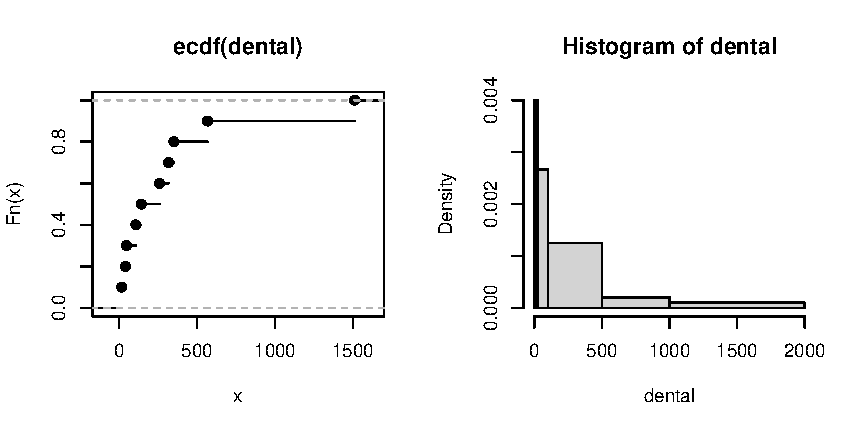
\includegraphics{cjs-rcs-figure}
%   \caption{\ifenglish A sample figure\else Exemple de figure\fi}
%   \label{fig:authguide:sample-figure}
% \end{figure}
%
% \ifenglish%
% If a figure requires an external file, you must provide it with your
% final version, usually in EPS, PDF or PNG format: see %
% \else%
% Si une figure requiert un fichier externe, vous devrez le fournir
% avec votre version finale, habituellement en format EPS, PDF ou PNG;
% consultez les %
% \fi
% \href{https://authorservices.wiley.com/author-resources/Journal-Authors/Prepare/manuscript-preparation-guidelines.html/figure-preparation.html}{%
%   \ifenglish Wiley's guidelines for the preparation of figures\relax
%   \else directives de Wiley pour la préparation des figures\fi}. %
%
% \ifenglish%
% Prepare tables as follows\relax%
% \else%
% Composez vos tableaux selon les règles suivantes\relax%
% \fi
% \footnote{%
%   \ifenglish%
%   These guidelines are adapted from the documentation of %
%   \else%
%   Ces règles sont adaptées de la documentation de %
%   \fi
%   \href{https://ctan.org/pkg/booktabs}{\pkg{booktabs}}.}: %
% \begin{itemize}
% \item %
%   \ifenglish%
%   no vertical lines; %
%   \else%
%   aucun filet vertical; %
%   \fi
% \item %
%   \ifenglish%
%   \cmdprint{\toprule} at the top; %
%   \else%
%   \cmdprint{\toprule} au début; %
%   \fi
% \item %
%   \ifenglish%
%   \cmdprint{\midrule} between the heading and body; %
%   \else%
%   \cmdprint{\midrule} entre l'entête et le corps; %
%   \fi
% \item%
%   \ifenglish%
%   \cmdprint{\bottomrule} at the bottom; %
%   \else%
%   \cmdprint{\bottomrule} au pied; %
%   \fi
% \item %
%   \ifenglish%
%   consistent number of decimal places thoughout the table; %
%   \else%
%   nombre de décimales uniforme; %
%   \fi
% \item %
%   \ifenglish%
%   leading digit in front of a decimal point ($0.1$, not $.1$).
%   \else%
%   marqueur des entiers devant les nombres décimaux ($0,1$ plutôt que
%   $,1$). %
%   \fi
% \end{itemize}
%
% \ifenglish%
% For table footnotes, use the package %
% \else%
% Pour les notes de contenu dans un tableau, utilisez %
% \fi%
% \href{https://ctan.org/pkg/threeparttable}{\pkg{threeparttable}}. %
% \ifenglish%
% However, place \cmdprint{\caption} \emph{outside} the environment
% \code{threeparttable} so that the caption can span the whole width
% of the page: %
% \else%
% Cependant, veillez à placer \cmdprint{\caption} à l'\emph{extérieur}
% de l'environnement \code{threeparttable} afin que la légende occupe
% toute la largeur de la page, le cas échéant: %
% \fi
% \iffalse
%<*example>
% \fi
  \def\CAPTION{\ifenglish caption\else légende\fi}
  \def\LABEL{\ifenglish label\else étiquette\fi}
  \def\TABLECONTENTS{\ifenglish table contents\else contenu du tableau\fi}
\begin{lstlisting}
\begin{table}
  \caption`\marg{\CAPTION}'
  \label`\marg{\LABEL}'
  \centering
  \begin{threeparttable}
    \begin{tabular}`\marg{cols}'
      `\meta{\TABLECONTENTS}'
    \end{tabular}
    \begin{tablenotes}
      `\meta{notes}'
    \end{tablenotes}
  \end{threeparttable}
\end{table}
\end{lstlisting}
% \iffalse
%</example>
% \fi
%
% \ifenglish%
% \section{Computer code and software}
% \else%
% \section{Code informatique et logiciels}
% \fi
% \label{sec:authguide:software}
%
% \ifenglish%
% Providing your computer code is a great way to increase the
% visibility of your work and its accessibility to end users of
% statistics. We strongly encourage that you share your code through a
% suitable repository, such as
% \else%
% Vous améliorerez la visibilité de vos travaux et leur dissémination
% parmi les utilisateurs de la statistique si vous fournissez votre
% code informatique. Nous vous encourageons fortement à partager
% celui-ci par le biais d'un dépôt ouvert, tel que %
% \fi
% \href{https://github.com/}{GitHub}
% \ifenglish or \else ou \fi %
% \href{https://gitlab.com/}{GitLab},
% \ifenglish%
% so that you can keep it up-to-date after the article has been
% published. Alternatively, you may provide your code in the
% Supplementary Material.
% \else%
% afin d'en permettre la mise à jour après la publication de
% l'article. Autrement, vous pouvez inclure le code dans le matériel
% additionnel. %
% \fi
%
% \ifenglish%
% The class does not offer any special features to typeset computer
% code. We recommend that you use specialized packages such
% as %
% \else%
% La classe ne propose aucune fonctionnalité particulière pour la
% présentation du code informatique. Nous vous recommandons d'avoir
% recours à des paquetages spécialisés comme %
% \fi
% \href{https://ctan.org/pkg/fancyvrb}{\pkg{fancyvrb}} %
% \ifenglish or \else ou \fi%
% \href{https://ctan.org/pkg/listings}{\pkg{listings}}. %
% \ifenglish%
% If you use {\Rlang} for your analysis, you could prepare the file
% using a literate programming system such as %
% \else%
% Si vous utilisez {\Rlang} pour effectuer votre analyse, vous pouvez
% rédiger l'article avec un système de programmation lettrée comme %
% \fi
% \href{https://en.wikipedia.org/wiki/Sweave}{Sweave} %
% \ifenglish or \else ou \fi%
% \href{https://en.wikipedia.org/wiki/Knitr}{knitr}.
%
% \ifenglish%
% That said, the class defines a few commands to ease and standardize
% the display of software names and code chunks. The command
% \cmd{\proglang} typesets the names of programming languages and
% software, and there are shortcuts for the most common cases; see
% \autoref{tab:authguide:proglang}. For example, refer to {\Rlang}
% using either \cmdprint{\proglang}\code{\{R\}} or
% \cmdprint{\Rlang}. The command \cmd{\pkg} typesets the names of
% software packages or modules. For example, refer to the {\Rlang}
% package \pkg{copula} using \cmdprint{\pkg}\code{\{copula\}}. %
% \else%
% Cela dit, la classe fournit quelques commandes pour faciliter et
% uniformiser la présentation des noms de logiciels et des extraits de
% code. La commande \cmd{\proglang} compose le nom des langages de
% programmation et des logiciels. Des raccourcis sont fournis pour les
% cas les plus usuels; voir le \autoref{tab:authguide:proglang}.
% Ainsi, pour mentionner {\Rlang}, utilisez
% \cmdprint{\proglang}\code{\{R\}} ou \cmdprint{\Rlang}. La commande
% \cmd{\pkg} compose le nom des paquetages ou modules logiciels. Par
% exemple, vous saisirez \cmdprint{\pkg}\code{\{copula\}} pour
% mentionner le paquetage {\Rlang} \pkg{copula}. %
% \fi
%
% \begin{table}
%   \ifenglish%
%   \caption{List of shortcuts for the names of programming languages
%   and software.}
%   \else%
%   \caption{Liste des raccourcis pour les noms de langages de
%   programmation et de logiciels}
%   \fi
%   \label{tab:authguide:proglang}
%   \centering
%   \begin{tabular}{ll}
%     \toprule
%     \ifenglish Software\else Logiciel\fi & \ifenglish Command\else Commande\fi \\
%     \midrule
%     \Rlang     & \cmd{\Rlang} \\
%     \SASlang   & \cmd{\SASlang} \\
%     \SPSSlang  & \cmd{\SPSSlang} \\
%     \Statalang & \cmd{\Statalang} \\
%     \Pylang    & \cmd{\Pylang} \\
%     \Julialang & \cmd{\Julialang} \\
%     \Clang     & \cmd{\Clang} \\
%     \Cpplang   & \cmd{\Cpplang} \\
%     \bottomrule
%   \end{tabular}
% \end{table}
%
% \ifenglish%
% For small chunks of code, such as the names of exploratory variables
% in a regression model, \cmd{\code} may be useful: it allows you to
% use the characters \code{_}, \code{~} and \code{$} directly. For
% example, you may write \cmdprint{\code}\code{\{patient_age\}} to get
% \code{patient_age}. %
% \else%
% La commande \cmd{\code} est utile pour composer de courts extraits
% de code, comme les noms des variables d'un modèle de régression. La
% commande permet d'utiliser directement les caractères «\code{_}»,
% «\code{~}» et «\code{$}». Par exemple, vous pouvez entrer
% \cmdprint{\code}\code{\{patient_age\}} pour obtenir
% \code{patient_age}. %
% \fi
%
% \ifenglish%
% Remember to report the software packages you used and their
% version numbers; see the following section. %
% \else%
% Vous devez toujours mentionner les logiciels utilisés, ainsi que
% leur version. La section suivante fournit plus de détails à ce
% sujet.
% \fi
%
% \ifenglish%
% \section{Citations and references}
% \else%
% \section{Citations et références}
% \fi
% \label{sec:authguide:references}
%
% \ifenglish%
% For citations and references, use {\BibTeX}. Recall that %
% \else%
% Utilisez {\BibTeX} pour les citations et les références. Tel que
% mentionné précédemment, le paquetage %
% \fi%
% \href{https://ctan.org/pkg/natbib}{\pkg{natbib}} %
% \ifenglish%
% is loaded automatically. Please use the \cmd{\citet} and
% \cmd{\citep} commands of \pkg{natbib}.
% \else%
% est chargé automatiquement par la classe. Assurez-vous
% d'utiliser ses commandes \cmd{\citet} et \cmd{\citep}. %
% \fi
%
% \ifenglish%
% The class also uses its own bibliography styles. These styles
% support the standard {\BibTeX} entry types %
% \else%
% La classe a également recours à ses propres styles de bibliographie.
% Ceux-ci prennent en charge les types d'entrées standards de
% {\BibTeX} %
% \fi
% (\code{article}, \code{book}, \code{proceedings}, etc.) %
% \ifenglish%
% and the standard fields %
% \else%
% et les champs standards %
% \fi%
% (\code{author}, \code{title}, \code{journal}, etc.). %
% \ifenglish%
% Furthermore, the styles support %
% \else%
% De plus, ils ajoutent les champs %
% \fi%
% \code{doi}, \code{isbn}, \code{url} \ifenglish and \else et \fi
% \code{language}.
% \ifenglish%
% These are explained in the examples below. %
% \else%
% Les exemples ci-dessous illustrent chacun de ces champs. %
% \fi%
%
% \begin{itemize}
% \item %
%   \ifenglish%
%   Articles with one author: \citet{Genest:1999}. To include a
%   DOI, use the field \code{doi} with a value in the format
%   \meta{prefix}\code{/}\meta{suffix} (for example,
%   \code{10.2307/3315650}). A hyperlink to the resource is then
%   created automatically. Note that journal names should not be
%   abbreviated. %
%   \else%
%   Articles avec un auteur unique: \citet{Genest:1999}. Pour ajouter
%   un identificateur DOI, utilisez le champ \code{doi} avec une valeur
%   de la forme \meta{préfixe}\code{/}\meta{suffixe} (par exemple:
%   \code{10.2307/3315650}). Un hyperlien vers la ressource est créé
%   automatiquement. Inscrivez les noms des journaux au long. %
%   \fi
% \item %
%   \ifenglish%
%   Articles with two authors: \citet{Qin/Lawless:1995}. Articles
%   with three or more authors: \citet{Davison/Fraser/Reid:2006} or
%   \citet{Granville:2023}. For articles with more than ten authors
%   \citep[such as][]{Teufel:2016}, give the first seven names
%   followed by ``and others''. {\BibTeX} will replace this by
%   ``et~al.''
%   \else%
%   Articles avec deux auteurs: \citet{Qin/Lawless:1995}. Articles
%   avec trois auteurs ou plus: \citet{Davison/Fraser/Reid:2006} ou
%   encore \citet{Granville:2023}. Pour les articles comptant plus de
%   dix auteurs \citep[par exemple:][]{Teufel:2016}, inscrivez les
%   noms des sept premiers auteurs, suivis de \emph{and others}.
%   {\BibTeX} inscrira automatiquement «et collab.» dans la notice.
%   \fi
% \item %
%   \ifenglish%
%   Use the field \code{language} for foreign-language articles, as in
%   \citet{Hoeffding:1940} (German) or
%   \citet{Ghoudi/Khoudraji/Rivest:1998} (French). Including this
%   information in the {\BibTeX} entry ensures that the title words
%   are hyphenated according to the rules of the corresponding
%   language. %
%   \else%
%   Le champ \code{language} permet d'indiquer la langue d'une notice
%   lorsqu'elle diffère de celle de l'article. C'est important pour la
%   coupure de mots dans les titres. Par exemple, pour le présent
%   document en français, la plupart des entrées de la bibliographie
%   déclarent l'anglais comme langue, alors que \citet{Hoeffding:1940}
%   déclare l'allemand. En revanche,
%   \citet{Ghoudi/Khoudraji/Rivest:1998} déclare le français pour la
%   version anglaise du document. %
%   \fi
% \item %
%   \ifenglish%
%   Books and other formats use the same author rules as articles.
%   An example of a book with two authors is
%   \citet{Kalbfleisch/Prentice:2002}. You may use \code{isbn} to include
%   the book's ISBN. Include the relevant page, section, or chapter
%   whenever possible in \cmd{\citet} and \cmd{\citep}. For example,
%   partial likelihood estimation in the Cox regression model may be
%   found in %
%   \else%
%   Les règles pour les auteurs de livres et autres types d'entrées
%   sont les mêmes que pour les articles.
%   \citet{Kalbfleisch/Prentice:2002} est un exemple de livre comptant
%   deux auteurs. Utilisez le champ \code{isbn} pour préciser le
%   numéro ISBN de l'ouvrage. Quand vous citez un livre, précisez
%   autant que faire se peut la page, la section ou le chapitre dans
%   les commandes \cmd{\citet} et \cmd{\citep}. Par exemple,
%   l'estimation par vraisemblance partielle dans le modèle de
%   régression de Cox est traitée dans %
%   \fi
%   \citet[\ifenglish Section\else section\fi~4.2]{Kalbfleisch/Prentice:2002}; %
%   \ifenglish see also \else voir aussi \fi %
%   \citet[\ifenglish Chapter\else chapitre\fi~6]{Kalbfleisch/Prentice:2002}.
% \item %
%   \ifenglish%
%   For references to articles in an edited book, include the page
%   numbers of the article, as well as the names of the book's
%   editors, such as \citet{Roberts:2009}. Again, we encourage you to
%   include the DOI. %
%   \else%
%   Pour la notice d'une partie d'un ouvrage collectif, précisez les
%   pages de la partie citée ainsi que les noms des éditeurs, tel que
%   dans \citet{Roberts:2009}. Ici aussi, nous vous invitons à inclure
%   un identificateur DOI. %
%   \fi
% \item %
%   \ifenglish%
%   You may need to cite a PhD thesis such as \citet{Syed:2022} or a
%   technical report such as \citet{Haas:2001} or an unpublished
%   manuscript posted on arXiv such as \citet{Tang/Kong/Wang:2023}.
%   If you have a DOI or URL, include it in the entry using \code{doi}
%   or \code{url}. If both are present in the database, the DOI
%   takes precedence.
%   \else%
%   Vous pouvez citer une thèse de doctorat \citep{Syed:2022}, un
%   rapport technique \citep{Haas:2001} ou une publication
%   préliminaire dans arXiv \citep{Tang/Kong/Wang:2023}. Saisissez les
%   identificateur DOI et les adresses URL avec les champs \code{doi}
%   et \code{url}. Lorsque les deux sont présents dans la base de
%   données, l'identificateur DOI a priorité. %
%   \fi
% \item %
%   \ifenglish%
%   Cite the software you used in your statistical analysis,
%   especially Free Software. To cite {\Rlang}, use the {\BibTeX}
%   entry provided by the command %
%   \else%
%   Citez les logiciels utilisés pour vos analyses statistiques, tout
%   particulièrement les logiciels libres. Pour citer {\Rlang},
%   utilisez l'entrée {\BibTeX} produite par la commande %
%   \fi
% \iffalse
%<*example>
% \fi
\begin{lstlisting}
> citation()
\end{lstlisting}
% \iffalse
%</example>
% \fi
%   \ifenglish%
%   Don't forget to include the version of {\Rlang}, as in:
%   ``Computations in this article were performed using {\Rlang}
%   \citep[v4.5.0]{Rlang}''. You can get this via:
%   \else%
%   N'oubliez pas d'inclure aussi la version de {\Rlang} dans une
%   mention de la forme «Les calculs de cet article ont été effectués
%   avec {\Rlang} \citep[v4.5.0]{Rlang}». L'expression {\Rlang}
%   suivante fournit la version du logiciel: %
%   \fi
% \iffalse
%<*example>
% \fi
\begin{lstlisting}
> R.version.string
\end{lstlisting}
% \iffalse
%</example>
% \fi
%   \ifenglish%
%   To cite an {\Rlang} package, use the command \code{citation} with
%   the name of the package in argument, e.g.\ %
%   \else%
%   Pour citer un paquetage {\Rlang}, utilisez aussi la commande
%   \code{citation}, mais en ajoutant le nom du paquetage en
%   argument: %
%   \fi
% \iffalse
%<*example>
% \fi
\begin{lstlisting}
> citation("copula")
\end{lstlisting}
% \iffalse
%</example>
% \fi
%   \ifenglish%
%   This specific example asks you to cite three articles
%   \citep{Yan:2007,Kojadinovic/Yan:2010,Hofert/Maechler:2011} as well
%   as the software itself \citep{Rcopula:2024}.
%   \else%
%   Dans cet exemple en particulier, on demande de citer trois
%   articles
%   \citep{Yan:2007,Kojadinovic/Yan:2010,Hofert/Maechler:2011} en plus
%   du logiciel lui-même \citep{Rcopula:2024}. %
%   \fi
% \item %
%   \ifenglish%
%   To cite data, please review %
%   \else%
%   Si vous devez citer des données, consultez la %
%   \fi
%   \href{https://authorservices.wiley.com/author-resources/Journal-Authors/open-access/data-sharing-citation/data-citation-policy.html}{%
%     \ifenglish Wiley's data citation policy\relax
%     \else politique de citation des données de Wiley\fi}. %
%   \ifenglish%
%   An example of a data citation is \citet{StatCan:2023}.
%   \else%
%   Un exemple de citation de données est \citet{StatCan:2023-fr}.
%   \fi
% \item %
%   \ifenglish%
%   You can also cite a webpage, for example \citet{Wolfram:2010}.
%   Include the date of access using the \code{note} field. %
%   \else%
%   Vous pouvez citer une page web, par exemple \citet{Wolfram:2010}.
%   Précisez la date de consultation de la page dans le champ
%   \code{note}. %
%   \fi
% \end{itemize}
%
% \appendix
%
% \ifenglish%
% \section{Proofs}
% \else%
% \section{Démonstrations}
% \fi
% \label{sec:authguide:proofs}
%
% \ifenglish%
% Appendices usually present original proofs or longer mathematical
% derivations; don't forget to cite them in the main article. You
% may structure each appendix into multiple sections and
% subsections. %
% \else%
% Les annexes sont habituellement réservées aux démonstrations ou
% longs développements mathématiques. Vous devez les citer dans le
% corps de l'article. Vous pouvez diviser les annexes en sections et
% sous-sections. %
% \fi
%
% \ifenglish%
% \section{Supplementary material}
% \else%
% \section{Matériel additionnel}
% \fi
% \label{sec:authguide:supplement}
%
% \ifenglish%
% To make your article accessible to a wide readership and to control
% its length, consider providing online supplementary material, citing
% it in the main article. It may contain additional simulation
% results, lengthy tables or figures, auxiliary results, proofs that
% are direct adaptations of calculations already published elsewhere,
% details about the code and software implementation, and so on. That
% said, we encourage you to place original mathematical proofs in an
% appendix and to present the ideas behind these proofs in the main
% text. %
% \else%
% Le matériel additionnel rendu disponible en ligne permet d'élargir
% le lectorat de votre article tout en limitant sa longueur. Vous
% devez citer le matériel additionnel dans l'article. Celui-ci peut
% contenir, entre autres, des résultats de simulation additionnels, de
% longs tableaux ou de grandes figures, des résultats auxiliaires, des
% démonstrations qui sont des applications directes de résultats déjà
% publiés ailleurs, des détails à propos de la mise en œuvre
% informatique. Attention, toutefois: les démonstrations originales
% sont mieux à leur place dans une annexe. Présentez simplement les
% idées fortes derrière celles-ci dans le corps du texte. %
% \fi
%
% \ifenglish%
% To prepare the supplementary material, use the option
% \code{supplement}: %
% \else%
% Pour préparer le matériel additionnel, utilisez l'option
% \code{supplement} de la classe: %
% \fi
% \iffalse
%<*example>
% \fi
\begin{lstlisting}
\documentclass[`\LANGOPT',supplement]{cjs-rcs-article}
\end{lstlisting}
% \iffalse
%</example>
% \fi
% \ifenglish%
% or, to make the supplement suitable for review, %
% \else%
% ou, pour anonymiser le matériel additionnel en vue de l'évaluation
% par les pairs,
% \fi
% \iffalse
%<*example>
% \fi
\begin{lstlisting}
\documentclass[`\LANGOPT',supplement,review]{cjs-rcs-article}
\end{lstlisting}
% \iffalse
%</example>
% \fi
% \ifenglish%
% Your supplementary material is published as supplied, and a proof is
% not made available, so be sure to double-check the file and to
% provide the material in its final format. %
% \else%
% Nous publions votre matériel additionnel tel quel; aucune épreuve ne
% vous sera fournie. Assurez-vous donc de la conformité de votre
% fichier. %
% \fi
%
% \vspace*{10pt}
% \hfill
% \ifenglish%
%   \emph{Have fun writing!}
% \else%
%   \emph{Bonne rédaction!}
% \fi%
%
% \begin{thebibliography}{23}
% \providecommand{\natexlab}[1]{#1}
% \providecommand{\url}[1]{\texttt{#1}}
% \providecommand{\urlprefix}{}
% \providecommand{\doiprefix}{doi: }
% \expandafter\ifx\csname href\endcsname\relax
%   \providecommand{\urldoi}[1]{#1}\else
%   \providecommand{\urldoi}[1]{\href{https://doi.org/#1}{#1}}\fi
% \providecommand{\selectlanguage}[1]{\relax}
% 
% \bibitem[{Davison et~al.(2006)Davison, Fraser, and
%   Reid}]{Davison/Fraser/Reid:2006}
% Davison, A.~C., Fraser, D. A.~S., and Reid, N. (2006).
% \newblock {\selectlanguage{english}Improved likelihood inference for discrete
%   data}.
% \newblock \emph{Journal of the Royal Statistical Society Series B: Statistical
%   Methodology}, 68(3):495--508.
% \newblock \doiprefix\urldoi{10.1111/j.1467-9868.2006.00548.x}.
% 
% \bibitem[{Downes and Beeton(2017)}]{Downes:short-math-guide:2017}
% Downes, M. and Beeton, B. (2017).
% \newblock {\selectlanguage{english}\emph{Short Math Guide for {\LaTeX}}}.
% \newblock American Mathematical Society.
% \newblock \urlprefix\url{https://ctan.org/pkg/short-math-guide}.
% 
% \bibitem[{Genest(1999)}]{Genest:1999}
% Genest, C. (1999).
% \newblock {\selectlanguage{english}Probability and statistics: A tale of two
%   worlds?}
% \newblock \emph{The Canadian Journal of Statistics}, 27(2):421--444.
% \newblock \doiprefix\urldoi{10.2307/3315650}.
% 
% \bibitem[{Ghoudi et~al.(1998)Ghoudi, Khoudraji, and
%   Rivest}]{Ghoudi/Khoudraji/Rivest:1998}
% Ghoudi, K., Khoudraji, A., and Rivest, L.-P. (1998).
% \newblock {\selectlanguage{french}Propri\'et\'es statistiques des copules de
%   valeurs extr\^emes bidimensionnelles}.
% \newblock \emph{The Canadian Journal of Statistics}, 26:187--197.
% \newblock \doiprefix\urldoi{10.2307/3315683}.
% 
% \bibitem[{Granville et~al.(2023)Granville, Woolford, Dean, Boychuk, and
%   McFayden}]{Granville:2023}
% Granville, K., Woolford, D.~G., Dean, C.~B., Boychuk, D., and McFayden, C.~B.
%   (2023).
% \newblock {\selectlanguage{english}On the selection of an interpolation method
%   with an application to the {F}ire {W}eather {I}ndex in {O}ntario, {C}anada}.
% \newblock \emph{Environmetrics}, 34(2):e2758.
% \newblock \doiprefix\urldoi{10.1002/env.2758}.
% 
% \bibitem[{Haas(2001)}]{Haas:2001}
% Haas, M. (2001).
% \newblock {\selectlanguage{english}\emph{New Methods in Backtesting}}.
% \newblock Tech. rep., Financial Engineering Research Center, Bonn, Germany.
% \newblock \urlprefix\url{https://www.yumpu.com/s/L9EC3aHSgRvWa763}.
% 
% \bibitem[{Higham(2020)}]{Higham:2020}
% Higham, N.~J. (2020).
% \newblock {\selectlanguage{english}\emph{Handbook of Writing for the
%   Mathematical Sciences}}.
% \newblock 3rd ed. SIAM, Philadelphia.
% \newblock ISBN 978-1-61197-609-0.
% \newblock \doiprefix\urldoi{10.1137/1.9781611976106}.
% 
% \bibitem[{Hoeffding(1940)}]{Hoeffding:1940}
% Hoeffding, W. (1940).
% \newblock {\selectlanguage{german}Ma{\ss}stabinvariante {K}orrelationstheorie
%   f\"ur diskontinuierliche {V}erteilungen}.
% \newblock \emph{Archiv f\"ur mathematische Wirtschafts- und Sozialforschung},
%   7:4--70.
% 
% \bibitem[{Hofert et~al.(2023)Hofert, Kojadinovic, Maechler, and
%   Yan}]{Rcopula:2024}
% Hofert, M., Kojadinovic, I., Maechler, M., and Yan, J. (2023).
% \newblock {\selectlanguage{english}\emph{copula: Multivariate Dependence with
%   Copulas}}.
% \newblock \urlprefix\url{https://cran.r-project.org/package=copula}.
% \newblock R package version 1.1-4.
% 
% \bibitem[{Hofert and M\"achler(2011)}]{Hofert/Maechler:2011}
% Hofert, M. and M\"achler, M. (2011).
% \newblock {\selectlanguage{english}Nested {A}rchimedean copulas meet {R}: The
%   {nacopula} package}.
% \newblock \emph{Journal of Statistical Software}, 39(9):1--20.
% \newblock \doiprefix\urldoi{10.18637/jss.v039.i09}.
% 
% \bibitem[{Kalbfleisch and Prentice(2002)}]{Kalbfleisch/Prentice:2002}
% Kalbfleisch, J.~D. and Prentice, R.~L. (2002).
% \newblock {\selectlanguage{english}\emph{The Statistical Analysis of Failure
%   Time Data}}.
% \newblock 2nd ed. Wiley Series in Probability and Statistics,
%   Wiley-Interscience [John Wiley \& Sons], Hoboken, NJ.
% \newblock ISBN 9780471363576.
% \newblock \doiprefix\urldoi{10.1002/9781118032985}.
% 
% \bibitem[{Kojadinovic and Yan(2010)}]{Kojadinovic/Yan:2010}
% Kojadinovic, I. and Yan, J. (2010).
% \newblock {\selectlanguage{english}Modeling multivariate distributions with
%   continuous margins using the {copula} {R} package}.
% \newblock \emph{Journal of Statistical Software}, 34(9):1--20.
% \newblock \doiprefix\urldoi{10.18637/jss.v034.i09}.
% 
% \bibitem[{Mermin(1989)}]{Mermin:1989}
% Mermin, N.~D. (1989).
% \newblock {\selectlanguage{english}What's wrong with these equations?}
% \newblock \emph{Physics Today}, 42(10):9--11.
% \newblock \doiprefix\urldoi{10.1063/1.2811173}.
% 
% \bibitem[{Oetiker et~al.(2021)Oetiker, Partl, Hyna, and
%   Schlegl}]{Oetiker:lshort-english:2021}
% Oetiker, T., Partl, H., Hyna, I., and Schlegl, E. (2021).
% \newblock {\selectlanguage{english}\emph{The Not So Short Introduction to
%   {\LaTeXe}}}.
% \newblock \urlprefix\url{https://ctan.org/pkg/lshort-english}.
% \newblock Version 6.4.
% 
% \bibitem[{Qin and Lawless(1995)}]{Qin/Lawless:1995}
% Qin, J. and Lawless, J. (1995).
% \newblock {\selectlanguage{english}Estimating equations, empirical likelihood
%   and constraints on parameters}.
% \newblock \emph{The Canadian Journal of Statistics}, 23(2):145--159.
% \newblock \doiprefix\urldoi{10.2307/3315441}.
% 
% \bibitem[{{R Core Team}(2024)}]{Rlang}
% {R Core Team} (2024).
% \newblock {\selectlanguage{english}\emph{R: A Language and Environment for
%   Statistical Computing}}.
% \newblock R Foundation for Statistical Computing, Vienna, Austria.
% \newblock \urlprefix\url{https://www.r-project.org/}.
% 
% \bibitem[{Roberts et~al.(2009)Roberts, Ren, and Rao}]{Roberts:2009}
% Roberts, G., Ren, Q., and Rao, J. N.~K. (2009).
% \newblock {\selectlanguage{english}Using marginal mean models for data from
%   longitudinal surveys with a complex design: Some advances in methods}.
% \newblock In R.~Lynn, editor, \emph{Methodology of Longitudinal Surveys}, pages
%   351--366. John Wiley \& Sons, New York.
% \newblock ISBN 9780470018712.
% \newblock \doiprefix\urldoi{10.1002/9780470743874}.
% 
% \bibitem[{{Statistics Canada}(2023)}]{StatCan:2023}
% {Statistics Canada} (2023).
% \newblock {\selectlanguage{english}Table 13-10-0096-01 {H}ealth
%   characteristics, annual estimates, inactive}.
% \newblock \doiprefix\urldoi{10.25318/1310009601-eng}.
% 
% \bibitem[{Syed(2022)}]{Syed:2022}
% Syed, S. (2022).
% \newblock {\selectlanguage{english}\emph{Non-reversible parallel tempering on
%   optimized paths}}.
% \newblock Ph.D. thesis, University of British Columbia, Vancouver (BC), Canada.
% \newblock \doiprefix\urldoi{10.14288/1.0413120}.
% 
% \bibitem[{Tang et~al.(2023)Tang, Kong, and Wang}]{Tang/Kong/Wang:2023}
% Tang, D., Kong, D., and Wang, L. (2023).
% \newblock {\selectlanguage{english}The synthetic instrument: From sparse
%   association to sparse causation}.
% \newblock arXiv.
% \newblock \doiprefix\urldoi{10.48550/arXiv.2304.01098}.
% 
% \bibitem[{Teufel et~al.(2016)Teufel, Diro, Whan, Milrad, Jeong, Ganji, Huziy
%   et~al.}]{Teufel:2016}
% Teufel, B., Diro, G.~T., Whan, K., Milrad, S.~M., Jeong, D.~I., Ganji, A.,
%   Huziy, O. et~al. (2016).
% \newblock {\selectlanguage{english}Investigation of the 2013 {A}lberta flood
%   from a weather/climate perspective}.
% \newblock \emph{Climate Dynamics}, 48(9):2881--2899.
% \newblock \doiprefix\urldoi{10.1007/s00382-016-3239-8}.
% 
% \bibitem[{{W}olfram {R}esearch(2010)}]{Wolfram:2010}
% {W}olfram {R}esearch (2010).
% \newblock {\selectlanguage{english}Pearson distribution}.
% \newblock
%   \urlprefix\url{https://reference.wolfram.com/language/ref/PearsonDistribution.html}.
% \newblock Accessed October 12, 2022.
% 
% \bibitem[{Yan(2007)}]{Yan:2007}
% Yan, J. (2007).
% \newblock {\selectlanguage{english}Enjoy the joy of copulas: With a package
%   copula}.
% \newblock \emph{Journal of Statistical Software}, 21(4):1--21.
% \newblock \doiprefix\urldoi{10.18637/jss.v021.i04}.
% 
% \end{thebibliography}
%
% \ifenglish%
%   \PrintChanges
% \else%
%   \section*{Historique des versions}
%   \label{sec:authguide:implementation}
%   Consultez la version anglaise de ce document pour l'historique des
%   versions. %
% \fi

%</fr-doc>
% \fi
% \GetFileInfo{cjs-rcs-authguide.dtx}
% \expandafter\parsedate\filedate\relax
%
% \changes{2.0}{2026-03-05}{Adapt the guidelines to the single-blind
% review process.}
% \changes{1.3}{2025-08-29}{Improve the French version in a few
% places.}
% \changes{1.2c}{2025-08-11}{Add guidelines on the length and contents
% of the abstracts.}
% \changes{1.2b}{2025-07-25}{Fix the link to instructions on updating
% a {\TeX} distribution.}
% \changes{1.2b}{2025-07-25}{Improve the text of the French version in
% a few places and fix typos.}
% \changes{1.2b}{2025-07-25}{Use the French variant of the reference
% Statistics Canada (2023) in the French version.}
% \changes{1.2a}{2025-07-24}{Fix the typesetting of a few entries in
% the list of references.}
% \changes{1.2a}{2025-07-24}{Provide more specific URLs for Oetiker et
% al. (2021) and Oetiker et collab. (2011).}
% \changes{1.2}{2025-07-10}{Initial version in the distribution.}
%
% \ifenglish%
% \makeatletter
% \title[Author guidelines for \CJS@journalname@en]{%
% Author guidelines \\ for \TheCJS}
% \makeatother
% \author{\SSCen}
% \affil{Guidelines developed by Julie Falkner, Vincent Goulet,
% Johanna Nešlehová}
% \runningauthor{Statistical Society of Canada}
% \else%
% \makeatletter
% \title[Directives pour les auteurs de \CJS@journalname@fr]{%
%   Directives pour les auteurs \\ de \LaRevue}
% \makeatother
% \author{\SSCfr}
% \affil{Directives rédigées par Julie Falkner, Vincent Goulet,
% Johanna Nešlehová}
% \runningauthor{Société canadienne de statistique}
% \fi
%
% \begin{englishabstract}
%   This guide provides the stylistic and presentation guidelines
%   for authors submitting an article to {\TheCJS}. Although the
%   guidelines apply broadly, the document assumes that the
%   manuscript is prepared using {\LaTeX} and the class
%   {\CJSclass}. This guide is also available in%
%   \ifenglish French\else English\fi.
% \end{englishabstract}
% \begin{frenchabstract}
%   Ce guide fournit les directives en matière de style et de
%   présentation pour les auteurs qui soumettent un article dans
%   {\LaRevue}. Les directives s'appliquent de manière générale, mais
%   le document se concentre sur la préparation d'un manuscript avec
%   {\LaTeX} et la classe {\CJSclass}. Ce guide est aussi disponible
%   en \ifenglish français\else anglais\fi.
% \end{frenchabstract}
%
% ^^A abusing the 'classification' environment. The final period is
% ^^A added by the environment.
% \begin{classification}[Version]
% \item[] %
%   \ifenglish%
%   These guidelines accompany the class {\CJSclass}~{\fileversion},
%   dated {\filedate} %
%   \else%
%   Ces directives accompagnent la classe {\CJSclass}~{\fileversion},
%   datée du {\filedate} %
%   \fi
% \end{classification}
%
% \licence{{\ccbysa*} 2025--{\year}, {\SSCen}~{\textbar}~{\SSCfr}}
%
% \makeCJStitle
%
% \section{Introduction}
% \label{sec:authguide:introduction}
%
% \ifenglish%
% This document provides guidelines for authors of {\TheCJS}. Please
% read them carefully: manuscripts that are scientifically acceptable
% but don't follow these stylistic guidelines will need additional
% work by the editors and copy-editors, delaying publication. %
% \else%
% Le présent document fournit les directives aux auteurs de
% {\LaRevue}. Lisez-le avec attention, car un manuscript
% scientifiquement acceptable verra sa publication retardée par le
% travail d'édition additionnel requis s'il ne respecte pas les
% directives en matière de style. %
% \fi
%
% \ifenglish%
% Manuscripts may be submitted in either English or French. We accept
% submissions in Microsoft~Word, but authors are encouraged to use
% {\LaTeX} and the class {\CJSclass}, described in this guide. You'll
% find documentation and additional information at the %
% \href{\siteurl}{project website}. %
% \else%
% Vous pouvez soumettre votre manuscript en français comme en anglais.
% Bien que nous acceptions le format Microsoft Word, nous recommandons
% d'utiliser {\LaTeX} et la classe {\CJSclass}. C'est d'ailleurs le
% mode de préparation décrit dans le présent guide. Vous trouverez de
% la documentation et des informations additionnelles dans le %
% \href{\siteurl/fr}{site web du projet}. %
% \fi%
%
% \ifenglish%
% Using {\CJSclass} requires an up-to-date {\TeX} distribution, so
% start by %
% \else%
% La classe {\CJSclass} requiert une distribution {\TeX} à jour, alors
% assurez-vous avant toute chose d'en %
% \fi
% \href{https://tex.stackexchange.com/q/55437}{\ifenglish doing this
% update\else effectuer la mise à jour\fi}. %
% \ifenglish%
% Since the class is part of the standard {\TeX} distributions via the
% package {\CJSpkg}, it will also get installed or updated. %
% \else
% Puisque la classe fait partie des distributions {\TeX} standards via
% le paquetage {\CJSpkg}, elle sera de ce fait installée ou mise à
% jour. %
% \fi
%
% \tipbox{%
%   \ifenglish%
%   If you get error messages about missing or outdated packages when
%   using {\CJSclass}, the solution is to update your {\TeX}
%   distribution. %
%   \else%
%   Si vous obtenez des messages d'erreur au sujet de paquetages
%   manquants ou obsolètes en utilisant {\CJSclass}, c'est que vous
%   devez mettre à jour de votre distribution {\TeX}. %
%   \fi}
%
% \ifenglish%
% \section{Preparing your article}
% \else%
% \section{Mise en place de l'article}
% \fi
% \label{sec:authguide:preparing}
%
% \ifenglish%
% Don't start from scratch. The class ships with templates for
% articles in English and French. If you're using the version included
% with your {\TeX} distribution, the templates are located with the
% documentation of the class. You may also obtain them from %
% \else%
% Ne partez pas de zéro. La classe est livrée avec des gabarits pour
% des articles en français et en anglais. Si vous utilisez la version
% fournie avec votre distribution {\TeX}, les gabarits sont classés
% avec la documentation de la classe. Vous pouvez aussi les récupérer
% depuis %
% \fi%
% \href{https://ctan.org/pkg/\CJSname}{CTAN}. %
% \ifenglish%
% Copy the template to your working directory and follow the
% instructions and examples therein. You may also compile the template
% as is, obtaining a complete sample article. %
% \else%
% Copiez le gabarit dans votre dossier de travail et suivez les
% directives et les exemples qui s'y trouvent. Vous pouvez compiler le
% gabarit tel quel pour produire un exemple d'article complet. %
% \fi
%
% \changes{1.3}{2025-08-27}{Instruct, in the introduction of
% \emph{Preparing your article}, to type non-ASCII characters directly
% rather than by using {\TeX} commands.}
% \ifenglish%
% If you need non-ASCII characters (such as accented letters) in your
% manuscript, type them directly instead of using {\TeX} commands
% (e.g.~\code{é} and \code{ü} instead of \code{{\bs}'e} and
% \code{{\bs}"u}), and save your file using %
% \else%
% Si vous avez recours à des caractères non-ASCII (comme des lettres
% accentuées), entrez directement ceux-ci au clavier, sans passer par
% les commandes {\TeX} (par exemple: «\code{é}» et «\code{ü}» plutôt
% que «\code{{\bs}'e}» et «\code{{\bs}"u}»). Enregistrez le fichier
% dans le codage de caractères %
% \fi%
% \href{https://fr.wikipedia.org/wiki/UTF-8}{UTF-8} %
% \ifenglish%
% character encoding. We recommend that you compile with {\LuaLaTeX},
% which allows for modern multilingual typesetting. Various packages
% are available with {\CJSclass} and there's no need to load them
% again: these include %
% \else%
% et compilez avec {\LuaLaTeX} pour tirer pleinement profit des
% caractéristiques de {\CJSclass}. Plusieurs paquetages étant chargés
% par la classe, vous n'avez pas besoin de les charger de nouveau.
% Parmi ceux-ci, mentionnons:%
% \fi
% \pkg{amsmath}, %
% \pkg{amsthm}, %
% \pkg{babel}, %
% \pkg{enumitem}, %
% \pkg{fontawesome5}, %
% \pkg{graphicx}, %
% \pkg{natbib}, %
% \pkg{numprint}, %
% \pkg{relsize}, %
% \pkg{url}\ifenglish, and \else\ et \fi %
% \pkg{xcolor}. %
%
% \ifenglish%
% \subsection{Class declaration}
% \else%
% \subsection{Déclaration de la classe}
% \fi
% \label{sec:authguide:preparing:documentclass}
%
% \ifenglish%
% The class requires the options \code{english} and \code{french}. The
% order is important: the \emph{second} one is the main language.
% Therefore, for an article in English use: %
% \else%
% Vous devez charger la classe avec les options \code{english} et
% \code{french}. Leur ordre est important: la \emph{seconde} est la
% langue principale de l'article. Par conséquent, pour un article en
% français, chargez la classe avec: %
% \fi
% \iffalse
%<*example>
% \fi
\def\LANGOPT{\ifenglish french,english\else english,french\fi}
\begin{lstlisting}
\documentclass[`\LANGOPT']{cjs-rcs-article}
\end{lstlisting}
% \iffalse
%</example>
% \fi%
%
% \ifenglish%
% \subsection{Title page}
% \else%
% \subsection{Page de titre}
% \fi
% \label{sec:authguide:preparing:titling}
%
% \ifenglish%
% Your preamble will contain the following declarations: %
% \else%
% Le préambule de votre manuscript doit contenir les déclarations
% suivantes pour produire les informations de la page de titre. %
% \fi
%
% \begin{itemize}
% \item %
%   \ifenglish%
%   \cmd{\title}: title of the article. See
%   \autoref{sec:authguide:typesetting:titles} for more on titles. Break a
%   long title covering more than one line using using \code{\bs\bs} or
%   \cmdprint{\newline}. If the title doesn't fit in the running head,
%   supply a short title as an optional argument (between square
%   brackets \texttt{[~]}): %
%   \else%
%   \cmd{\title}: titre de l'article; voir la
%   \autoref{sec:authguide:typesetting:titles} pour des détails
%   additionnels sur la composition du titre. Coupez manuellement un
%   titre qui nécessite plus d'une ligne avec \code{\bs\bs} ou
%   \cmdprint{\newline}. Si le titre est trop long pour l'entête,
%   fournissez une version courte en argument optionnel (entre les
%   crochets \texttt{[~]}): %
%   \fi%
%   \iffalse
%<*example>
%   \fi
\def\OPT{\ifenglish Short title\else Titre court\fi}
\def\ARG{\ifenglish Full title\else Titre complet\fi}
\begin{lstlisting}
\title`\oarg{\OPT}\marg{\ARG}'
\end{lstlisting}
%   \iffalse
%</example>
%   \fi
% \item %
%   \ifenglish%
%   \cmd{\author} and \cmd{\affil}: author name, ORCID~iD, email and
%   affiliation (give the country name in the language of the
%   article). The corresponding author is specified by
%   \code{corresponding} and surnames via \cmd{\surname}: %
%   \else%
%   \cmd{\author} et \cmd{\affil}: noms, identifiants ORCID, adresses
%   courriel et affiliations des auteurs (indiquez le nom du pays dans
%   la langue de l'article). Indiquez l'auteur correspondant avec
%   \code{corresponding} et entrez les noms de famille avec
%   \cmd{\surname}: %
%   \fi%
%   \iffalse
%<*example>
%   \fi
\def\EMAIL{\ifenglish email\else courriel\fi}
\def\FORENAME{\ifenglish Forename\else Prénom\fi}
\def\SURNAME{\ifenglish Surname\else Nom\fi}
\def\AFFIL{\ifenglish Department, University, City, Country\else%
  Département, Université, Ville, Pays\fi}
\begin{lstlisting}
\author[orcid=`\meta{id}', email=`\meta{\EMAIL}', corresponding]
       {`\meta{\FORENAME}' \surname`\marg{\SURNAME}'}
\affil`\marg{\AFFIL}'
\end{lstlisting}
%   \iffalse
%</example>
%   \fi
%
%   \ifenglish%
%   To acknowledge the Alzheimer’s Disease Neuroimaging Initiative
%   (ADNI), insert \cmd{\ADNIacknowledgement} after the declarations
%   of the authors and the class will add the required statement on
%   the title page. Similarly, \cmd{\ADMCacknowledgement} acknowledges
%   the Alzheimer’s Disease Metabolomics Consortium (ADMC).%
%   \else%
%   Pour reconnaitre la contribution de l'Alzheimer’s Disease
%   Neuroimaging Initiative (ADNI), insérez la commande
%   \cmd{\ADNIacknowledgement} après les définitions de tous les
%   auteurs. La classe se chargera  d'ajouter la déclaration
%   obligatoire dans la page de titre. De manière analogue, la
%   commande \cmd{\ADMCacknowledgement} reconnait la contribution du
%   Alzheimer’s Disease Metabolomics Consortium (ADMC). %
%   \fi
% \item %
%   \ifenglish%
%   \code{englishabstract} and \code{frenchabstract} environments: the
%   required English and French abstracts. These should be concise;
%   the English abstract must not exceed 20~lines in the format of the
%   class. We strongly discourage symbols, formulas and citations in
%   the abstracts. If you ask us to, we'll prepare a French abstract
%   for your English-language article. The order of these declarations
%   is not important: %
%   \else%
%   environnements \code{frenchabstract} et \code{englishabstract}:
%   résumés français et anglais. Ceux-ci doivent être concis: la
%   version anglaise ne doit pas dépasser 20~lignes dans le format de
%   la classe. Les symboles, formules mathématiques et citations sont
%   fortement déconseillées dans les résumés. Nous vous fournirons sur
%   demande un résumé en anglais pour un article en français. L'ordre
%   des déclarations n'a pas d'importance: %
%   \fi
%   \iffalse
%<*example>
%   \fi
\begin{lstlisting}
\begin{englishabstract}
  `\meta{Text of the English abstract}'
\end{englishabstract}

\begin{frenchabstract}
  `\meta{Texte du résumé en français}'
\end{frenchabstract}
\end{lstlisting}
%   \iffalse
%</example>
%   \fi
% \item %
%   \ifenglish%
%   \code{keywords} environment: the list of keywords. Capitalize
%   only the first keyword, order them alphabetically, and don't include
%   any punctuation: %
%   \else%
%   environnement \code{keywords}: liste de mots-clés. Saisissez les
%   mots-clés en ordre alphabétique, avec une majuscule uniquement
%   pour le premier et sans aucune ponctuation: %
%   \fi%
%   \iffalse
%<*example>
%   \fi
\def\KEYWORDC{\ifenglish Keyword\else Mot-clé\fi}
\def\KEYWORD{\ifenglish keyword\else mot-clé\fi}
\begin{lstlisting}
\begin{keywords}
\item `\normalfont\itshape{\KEYWORDC} 1'
\item `\normalfont\itshape{\KEYWORD} 2'
...
\end{keywords}
\end{lstlisting}
%   \iffalse
%</example>
%   \fi
% \item %
%   \ifenglish%
%   \code{classification} environment: the %
%   \else%
%   environnement \code{classification}: classification mathématique
%   par matières selon le classement %
%   \fi
%   \href{https://msc2020.org}{MSC2020}\ifenglish{ }\else. \fi %
%   \ifenglish%
%   mathematics subject classification. Provide primary and secondary
%   classifications: %
%   \else
%   Indiquez des classifications primaires et secondaires: %
%   \fi
%   \iffalse
%<*example>
%   \fi
\def\PRIMARY{\ifenglish Primary\else Primaire\fi}
\def\SECONDARY{\ifenglish Secondary\else Secondaire\fi}
\def\CODE{\ifenglish code\else rubrique\fi}
\begin{lstlisting}
\begin{classification}
\item[`\PRIMARY'] `\normalfont\itshape{\CODE} 1, {\CODE} 2, \dots'
\item[`\SECONDARY'] `\normalfont\itshape{\CODE} 1, {\CODE} 2, \dots'
\end{classification}
\end{lstlisting}
%   \iffalse
%</example>
%   \fi
% \end{itemize}
%
% \ifenglish%
% \subsection{Back matter}
% \else%
% \subsection{Informations des parties annexes}
% \fi
% \label{sec:authguide:preparing:backmatter}
%
% \ifenglish%
% Articles end with the data sharing statement, acknowledgements,
% etc., and you may also enter these details in the preamble using the
% environments below. Note that ORCID identifiers appear
% automatically. %
% \else%
% Les articles se terminent par des parties annexes contenant les
% conditions de partage des données, les remerciements, etc. Nous vous
% recommandons de saisir ces informations dans le préambule à l'aide
% des environnements ci-dessous. Les identifiants ORCID sont quant à
% eux affichés automatiquement. %
% \fi
%
% \begin{itemize}
% \item %
%   \ifenglish%
%   \code{supplement}: if you have online supplementary
%   material, this is the place to describe it. For example, the
%   Supplementary Material contains auxiliary technical lemmas, a
%   detailed description of the simulation study, and additional
%   simulation results. %
%   \else%
%   \code{supplement}: liste de votre matériel additionnel disponible
%   en ligne, le cas échéant. Le matériel additionnel peut, par exemple,
%   contenir des lemmes techniques supplémentaires, une description
%   détaillée d'une étude de simulation ou des résultats de simulation
%   additionnels. %
%   \fi
% \item %
%   \def\POLICYNAME{\ifenglish Expects Data Sharing\else \emph{Expects Data Sharing}\fi}
%   \ifenglish%
%   \code{sharing}: statement about the availability or absence of
%   shared data. Provide a DOI or URL for the latter, as per our %
%   \else%
%   \code{sharing}: conditions de partage des données de recherche ou
%   explication de leur absence. En vertu de notre politique
%   éditoriale %
%   \fi%
%   \href{https://authorservices.wiley.com/author-resources/Journal-Authors/open-access/data-sharing-citation/data-sharing-policy.html}{\POLICYNAME}\ifenglish{ }\else, \fi %
%   \ifenglish%
%   policy. If there are ethical or legal concerns, we encourage you
%   to provide synthetic data instead. You may also use the
%   environment to describe how to access your code. If data sharing
%   is not applicable, write: ``Data sharing not applicable to this
%   article as no datasets were generated or analyzed during the
%   current study.'' %
%   \else%
%   vous devez fournir un lien permanent vers les données
%   (identificateur DOI ou adresse URL). En cas d'enjeux éthiques ou
%   légaux, utilisez si possible des données de synthèse. Vous pouvez
%   aussi utiliser l'environnement pour indiquer comment accéder à
%   votre code informatique. Si le partage des données ne s'applique
%   pas, écrivez: «Le partage des données ne s'applique pas à cet
%   article car aucun jeu de données n'a été généré au analysé au
%   cours de l'étude.» %
%   \fi
% \item %
%   \ifenglish%
%   \code{acknowledgements}: has a colleague or supervisor provided
%   crucial help or expertise? %
%   \else%
%   \code{acknowledgements}: remerciements, si vous avez obtenu de
%   l'aide cruciale de la part de collègues ou de superviseurs. %
%   \fi%
% \item %
%   \ifenglish%
%   \code{funding}: include your funding information here, and don't
%   abbreviate the names of granting agencies. %
%   \else%
%   \code{funding}: informations sur le financement de la recherche.
%   Indiquez le nom des agences de financement au long. %
%   \fi
% \end{itemize}
%
% \changes{2.0}{2026-02-23}{Section \emph{Anonymous version} becomes
% \emph{Peer review version}, with all anonymity-related material
% deleted.}
% \ifenglish%
% \subsection{Peer review version}
% \else%
% \subsection{Version pour évaluation}
% \fi%
% \label{sec:authguide:preparing:review}
%
% \ifenglish%
% {\TheCJS} uses a single-blind peer review process. Until acceptance,
% please prepare your manuscript using the class option \code{review}
% as follows: %
% \else%
% {\LaRevue} procède à l'évaluation par les pairs en simple anonymat.
% Composez la version de votre manuscrit pour évaluation avec l'option
% \code{review}: %
% \fi%
% \iffalse
%<*example>
% \fi
\begin{lstlisting}
\documentclass[`\LANGOPT',review]{cjs-rcs-article}
\end{lstlisting}
% \iffalse
%</example>
% \fi%
% \changes{1.3}{2025-08-27}{Emphasize in section \emph{Anonymous
% version} that acknowledgements, funding information and ORCID iDs is
% among the information hidden by option \texttt{review}.}
% \ifenglish%
% The option numbers the lines and increases the line spacing. It
% should also be used for your supplementary document; see
% \autoref{sec:authguide:supplement}. After acceptance, remove the
% \code{review} option and compile twice to remove the line numbers. %
% \else%
% L'option numérote les lignes et augmente l'interligne. Vous
% devriez aussi l'utiliser pour le matériel additionnel; voir
% l'\autoref{sec:authguide:supplement}. Une fois votre article accepté
% pour publication, retirez l'option \code{review} et compilez
% au moins deux fois pour annuler l'effet de la numérotation des
% lignes. %
% \fi
%
% \ifenglish%
% Referees and editors may check the literature for overlaps with your
% research. Therefore, provide DOIs, arXiv~IDs, or article numbers in
% the list of references to ease retrieval. If your manuscript is
% based on your thesis, there will be overlap, so ask yourself if you
% really need a reference. Refer to the thesis only if you use
% unpublished results from it that are not included in the current
% manuscript. %
% \else%
% Les arbitres et les éditeurs vérifieront si votre travail recoupe
% des résultats déjà présents dans la littérature. Veillez donc à
% fournir pour vos références des identificateurs DOI ou arXiv,
% ou encore des numéros d'articles, afin d'en faciliter le repérage.
% Les recoupements étant inévitables si l'article est tiré de votre
% thèse, demandez-vous si une référence à celle-ci est vraiment
% nécessaire. Elle ne le sera que si l'article fait appel à des
% résultats de la thèse qui n'ont pas été publiés ailleurs. %
%\fi
%
% \ifenglish%
% We allow submissions of arXiv preprints. %
% \else%
% Vous pouvez soumettre une publication préliminaire arXiv. %
% \fi
%
% \ifenglish%
% \subsection{Repository version}
% \else%
% \subsection{Version préliminaire}
% \fi%
% \label{sec:authguide:preparing:nocjs}
%
% \ifenglish%
% To prepare a version of your article for a repository such as arXiv,
% use the \code{nocjs} option:
% \else%
% Pour créer une version préliminaire de votre article pour
% publication dans une archive ouverte telle que arXiv, utilisez
% l'option \code{nocjs}: %
% \fi%
% \iffalse
%<*example>
% \fi
\begin{lstlisting}
\documentclass[`\LANGOPT',nocjs]{cjs-rcs-article}
\end{lstlisting}
% \iffalse
%</example>
% \fi
%
% \ifenglish%
% \section{Length restrictions}
% \else%
% \section{Longueur maximale}
% \fi
% \label{sec:authguide:length}
%
% \ifenglish%
% Your submission should not exceed 32~pages when compiled with the
% \code{review} option, and this is enforced when a revision is
% invited. It's harder to find reviewers for overly long manuscripts
% and they'll need more time, causing delays throughout the process. %
% \else%
% Votre proposition ne devrait pas excéder 32~pages lorsque composée
% avec l'option \code{review}. Gardez en tête que les longs articles
% compliquent le recrutement d'arbitres et allongent le processus
% de révision, ce qui à terme retarde la publication de votre
% article. %
% \fi
%
% \ifenglish%
% Concise abstracts are preferred. The English version must not
% exceed 20~lines. %
% \else%
% Visez la concision pour vos résumés. La version anglaise ne devrait
% pas dépasser 20~lignes.
% \fi
%
% \ifenglish%
% Lengthy mathematical derivations and proofs are better placed in the
% appendices (see \autoref{sec:authguide:proofs}). Relevant material
% that doesn't belong in the main article can be included in the
% Supplementary Material (see \autoref{sec:authguide:supplement}). %
% \else%
% Les longs développements mathématiques et les longues démontrations
% sont mieux à leur place en annexe (consultez
% l'\autoref{sec:authguide:proofs}). Vous pouvez placer les autres
% éléments utiles, mais non essentiels dans le matériel
% additionnel (voir l'\autoref{sec:authguide:supplement}). %
% \fi
%
% \ifenglish%
% \section{Article structure}
% \else%
% \section{Structure de l'article}
% \fi
% \label{sec:authguide:structure}
%
% \ifenglish%
% Our templates will guide you through the following structure: %
% \else%
% Suivez nos gabarits, ils vous guideront vers la structure suivante: %
% \fi
% \begin{itemize}
% \item %
%   \ifenglish%
%   The title page created with \cmd{\maketitle}. %
%   \else%
%   La page de titre produite avec \cmd{\maketitle}. %
%   \fi
% \item %
%   \ifenglish%
%   The introduction. %
%   \else%
%   L'introduction. %
%   \fi
% \item %
%   \ifenglish%
%   The body divided into sections using %
%   \else%
%   Le corps de l'article découpé en sections avec %
%   \fi
%   \cmd{\section}, %
%   \cmd{\subsection} %
%   \ifenglish and \else et \fi%
%   \cmd{\subsubsection}. %
% \item %
%   \ifenglish%
%   (Optional) The conclusion, if it contains new material; don't
%   just repeat the content of the article. %
%   \else%
%   (Optionnel) La conclusion, dans la mesure où elle propose
%   quelque chose de nouveau. Ne réitérez pas simplement le contenu de
%   l'article. %
%   \fi
% \item %
%   \ifenglish%
%   The back matter created with \cmd{\makebackmatter}. %
%   \else%
%   Les parties annexes produites avec la commande
%   \cmd{\makebackmatter}. %
%   \fi
% \item %
%   \ifenglish%
%   (Optional) The command \cmd{\appendix}, followed by the appendices.
%   Cite each appendix in the main article. %
%   \else%
%   (Optionnel) La commande \cmd{\appendix}, suivie des annexes. Citez
%   chacune des annexes dans l'article. %
%   \fi
% \item %
%   \ifenglish%
%   The  reference list created with \cmd{\bibliography}. %
%   \else%
%   La liste des références produite avec \cmd{\bibliography}. %
%   \fi
% \end{itemize}
%
% \ifenglish%
% \section{General typesetting}
% \else%
% \section{Composition et mise en page}
% \fi
% \label{sec:authguide:typesetting}
%
% \ifenglish%
% It's your responsibility to submit a manuscript in accordance with
% our presentation rules. Keep the {\LaTeX} code as simple as
% possible, and avoid including packages or defining commands that are
% not necessary. %
% \else%
% Vous avez la responsabilité de présenter un manuscript qui respecte
% nos règles de présentation matérielle. Gardez le code {\LaTeX}
% simple, ne chargez pas de paquetages inutiles et évitez de définir
% des commandes inutilisées. %
% \fi
%
% \ifenglish%
% In your writing, try to be clear and concise, avoiding empty phrases
% that add nothing. Use footnotes sparingly, and avoid any
% mathematical expressions in them. Likewise, use italics for emphasis
% only when really needed.
% \else%
% Rédigez de manière claire et concise, sans phrases creuses qui
% n'apportent rien au propos. Limitez le recours aux notes de bas
% de page et évitez qu'elles ne contiennent des expressions
% mathématiques. De même, soulignez par de l'italique uniquement
% lorsque nécessaire.
% \fi
%
% \ifenglish%
% \subsection{Margins and page layout}
% \else%
% \subsection{Marges et mise en page}
% \fi
% \label{sec:authguide:typesetting:margins}
%
% \ifenglish%
% Do not change the page layout, margins, fonts, or character
% encoding. Note that the package \pkg{geometry} is incompatible with
% {\CJSclass}. %
% \else%
% Ne modifiez pas la mise en page, les marges, les polices de
% caractères ou le codage des caractères. Le paquetage \pkg{geometry}
% est d'ailleurs incompatible avec {\CJSclass}. %
% \fi
%
% \ifenglish%
% \subsection{Article title and section titles}
% \else
% \subsection{Titres}
% \fi
% \label{sec:authguide:typesetting:titles}
%
% \ifenglish%
% The article title as well as section and subsection titles are
% written in sentence style, that is, with only an initial capital. In
% English, also capitalize the first word after a colon. Make sure the
% title is no more than two lines long, and give a shorter version for
% the running head if ncessary. %
% \else%
% Entrez le titre de l'article ainsi que les titres de sections en
% minuscules (sauf pour la majuscule initiale). En anglais, utilisez
% toutefois une majuscule initiale après un deux-points. Assurez-vous
% que la longueur du titre n'excède pas deux lignes et fournissez une
% version courte pour l'entête si nécessaire. %
% \fi
%
% \ifenglish
% Avoid mathematical formulas in the article title and section titles.
% If you do need a section title with a mathematical symbol, read
% \nolink{\autoref{sec:hyperlinks}} of the class documentation. %
% \else%
% Évitez d'utiliser de la notation mathématique dans le titre de
% l'article et dans les titres de sections. Si vous ne pouvez faire
% autrement, consultez la \nolink{\autoref{sec:hyperlinks}} de la
% documentation de la classe. %
% \fi
%
% \ifenglish%
% \subsection{Cross-references}
% \else%
% \subsection{Renvois}
% \fi%
% \label{sec:authguide:typesetting:references}
%
% \ifenglish%
% Manual references to sections, theorems, equations, etc. are not
% acceptable. Instead use the cross-reference system of {\LaTeX}
% \citep[Section~2.8]{Oetiker:lshort-english:2021}, but using the
% command \cmd{\autoref} to automatically insert a descriptor: %
% \else%
% Les renvois manuels vers des sections, théorèmes, équations, etc.,
% ne sont pas permis. Utilisez le système de renvois (ou références
% croisées) de {\LaTeX}
% \citep[Section~2.8]{Oetiker:lshort-french:2011}, mais à l'aide de la
% commande \cmd{\autoref} qui ajoute automatiquement une
% description: %
% \fi
% \begin{quote}
%   \def\TEXT{\ifenglish as seen in \else tel qu'abordé à la \fi}
%   \def\LABEL{\ifenglish label\else étiquette\fi}
%   \code{\TEXT}\cmdprint{\autoref}\marg{\LABEL}
%   \quad$\rightarrow$\quad
%   \TEXT \autoref{sec:authguide:length}
% \end{quote}
% \ifenglish%
% The exception to this rule is equations, where you choose the
% appropriate descriptor; see
% \autoref{sec:authguide:mathematics:tips}. %
% \else%
% L'exception à cette règle: les équations, pour lesquelles vous devez
% ajouter la description vous-même; consultez la
% \autoref{sec:authguide:mathematics:tips}. %
% \fi
%
% \ifenglish
% \subsection{English spelling}
% \else
% \subsection{Orthographe anglaise}
% \fi
% \label{sec:authguide:typesetting:spelling}
%
% \ifenglish%
% We follow the style of the \emph{Canadian Oxford Dictionary} for
% English spelling. If the dictionary lists more than one acceptable
% spelling, choose the main entry. Here are a few more helpful
% hints: %
% \else%
% Si vous rédigez en anglais, respectez l'orthographe du
% \emph{Canadian Oxford Dictionary}. Si l'ouvrage cite plusieurs
% variantes orthographiques pour un mot, optez pour celle de l'entrée
% principale. Voici quelques conseils additionnels: %
% \fi
% \begin{itemize}
% \item %
%   \ifenglish%
%   The word \textit{data} is plural, and so it should be followed
%   by a plural verb.
%   \else%
%   Le mot \emph{data} est pluriel et, par conséquent, il doit être
%   accompagné d'un verbe au pluriel. %
%   \fi
% \item %
%   \ifenglish%
%   Avoid unnecessary hyphens: we prefer \textit{nonlinear} and
%   \textit{semiparametric} to the hyphenated alternatives.
%   \else%
%   Évitez les traits d'union inutiles: nous favorisons
%   \textit{nonlinear} et \textit{semiparametric} à leur alternative
%   avec trait d'union. %
%   \fi
% \item %
%   \ifenglish%
%   Avoid nonstandard abbreviations, particularly of specialized
%   statistical tools, or abbreviations that are part of a
%   subject-matter jargon. This may slightly increase the length of
%   your article, but it will be easier to read and more accessible
%   for those who are not experts in your area.
%   \else%
%   Évitez d'utiliser des abréviations non usuelles~--- notamment
%   d'outils statistiques spécialisés~--- ou qui relèvent du jargon
%   technique d'un domaine en particulier. En échange d'une longueur
%   légèrement accrue, votre article s'en trouvera plus facile à lire.
%   Ceci s'applique évidemment aussi à la rédaction en français. %
%   \fi
% \item %
%   \ifenglish%
%   The abbreviation ``cf.'' means ``compare to'' and not ``refer
%   to''. If you mean ``refer to'', just write ``see''. %
%   \else%
%   L'abréviation \emph{cf.} signifie \emph{compare to}, et non
%   \emph{refer to}. Pour cette seconde expression, utilisez
%   simplement \emph{see}. %
%   \fi
% \end{itemize}
%
% \ifenglish%
% If you're not sure about something, look it up. Helpful books include
% \citet{Higham:2020}, and there are many online resources to help you
% improve your writing, such as
% \else%
% En cas de doute, consultez des ouvrages de référence. En
% particulier, nous vous recommandons \citet{Higham:2020}. Il existe
% aussi de nombreuses ressources en ligne, tel que %
% \fi
% \href{https://www.cs.columbia.edu/~hgs/etc/writing-bugs.html}{%
%   \emph{Common Bugs in Writing}}
% \ifenglish by \else de \fi %
% Henning Schulzrinne.
%
% \ifenglish%
% \subsection{French typesetting}
% \else%
% \subsection{Rédaction en français}
% \fi
% \label{sec:authguide:typesetting:french}
%
% \ifenglish%
% {\TheCJS} allows submissions in French. The class fully supports
% French typesetting when you load the class with %
% \iffalse
%<*example>
% \fi
\begin{lstlisting}
\documentclass[english,french]{cjs-rcs-article}
\end{lstlisting}
% \iffalse
%</example>
% \fi
% (The other options \code{review} and \code{nocjs} remain available.)
% The position of the abstracts will be swapped, French set as the
% default language, and the bibliography style changed. See
% \nolink{\autoref{sec:usage:french}} of the class documentation. %
% \else%
% Vous pouvez soumettre un article pour publication en français dans
% {\LaRevue}. La classe est entièrement adaptée à la rédaction dans
% cette langue. Consultez à cet effet la
% \nolink{\autoref{sec:usage:french}} de la documentation de la
% classe. %
% \fi
%
% \ifenglish%
% \section{Mathematics}
% \else%
% \section{Mathématiques}
% \fi
% \label{sec:authguide:mathematics}
%
% \ifenglish%
% Unless central or essential to the flow of the discussion, lengthy
% mathematical arguments should be deferred to an appendix or the
% supplementary material. The same applies to lengthy lists of
% regularity conditions. However, important ideas behind original
% proofs that help the reader to follow and appreciate your results
% should be included in the main body of the manuscript. %
% \else%
% À moins qu'ils ne s'avèrent essentiels à la discussion, placez les
% longs développements mathématiques en annexe ou dans le matériel
% additionnel. Il en va de même des longues listes de conditions de
% régularité. En revanche, vous pouvez inclure dans le corps de
% l'article les idées fortes que les lecteurs devraient connaitre pour
% bien suivre une démonstration. %
% \fi
%
% \ifenglish%
% \subsection{Operators and symbols}
% \else%
% \subsection{Opérateurs et symboles}
% \fi
% \label{sec:authguide:mathematics:operators}
%
% \ifenglish%
% The class loads %
% \else%
% La classe charge d'office %
% \fi%
% \href{https://ctan.org/pkg/amsmath}{\pkg{amsmath}}\ifenglish{} \else, \fi%
% \ifenglish%
% automatically, as well as %
% \else%
% ainsi que %
% \fi%
% \href{https://ctan.org/pkg/unicode-math}{\pkg{unicode-math}} %
% \ifenglish%
% when the document is compiled with {\LuaLaTeX}. However, it isn't
% compatible with \pkg{amssymb}. %
% \else%
% lorsque le document est compilé avec {\LuaLaTeX}. Cependant, elle
% n'est pas compatible avec \pkg{amssymb}. %
% \fi
%
% \ifenglish%
% {\LaTeX} provides many commands to typeset common mathematical
% symbols and operators \citep[see][]{Downes:short-math-guide:2017}. The
% class provides the additional commands summarized in
% \autoref{tab:authguide:math} and explained below: %
% \else%
% {\LaTeX} définit plusieurs commandes pour composer les symboles
% et opérateurs mathématiques usuels
% \citep{Downes:short-math-guide:2017}. La classe définit pour sa part
% les commandes suivantes, résumées dans le
% \autoref{tab:authguide:math}: %
% \fi
%
% \begin{table}
%   \ifenglish%
%   \caption{Additional commands for mathematical symbols and
%   operators defined by {\CJSclass}}
%   \else%
%   \caption{Commandes additionnelles pour les symboles et opérateurs
%   mathématiques définies par {\CJSclass}}
%   \fi
%   \label{tab:authguide:math}
%   \centering
%   \begin{threeparttable}
%     \begin{tabular}{llll}
%       \toprule
%       \ifenglish Command\else Commande\fi & Description &
%       \ifenglish Example\else Exemple\fi &
%       \ifenglish Output\else Résultat\fi \\
%       \midrule
%       \cmd{\Pr} &
%       \ifenglish probability\else probabilité\fi\tnote{a} &
%       \cmdprint{\Pr}\code{[X = x]} & $\Pr[X = x]$ \\
%       \cmd{\E} &
%       \ifenglish expected value\else espérance\fi &
%       \cmdprint{\E}\code{[X]} & $\E[X]$ \\
%       \cmd{\Var} &
%       variance &
%       \cmdprint{\Var}\code{[X]} & $\Var[X]$ \\
%       \cmd{\Cov} &
%       covariance &
%       \cmdprint{\Cov}\code{(X, Y)} & $\Cov(X, Y)$ \\
%       \cmd{\corr} &
%       \ifenglish correlation\else corrélation\fi &
%       \cmdprint{\corr}\code{(X, Y)} & $\corr(X, Y)$ \\
%       \cmd{\prdist} &
%       \ifenglish probability distribution\else loi de probabilité\fi &
%       \cmdprint{\prdist}\code{\{N\}} & $\prdist{N}$ \\
%       \addlinespace
%       \cmd{\mat} &
%       \ifenglish matrix or vector\else matrice ou vecteur\fi &
%       \cmdprint{\mat}\code{\{A\}} & $\mat{A}$ \\
%       \cmd{\matit} &
%       \ifenglish matrix or vector (italic)\else matrice ou vecteur (italique)\fi &
%       \cmdprint{\matit}\code{\{x\}} & $\matit{x}$ \\
%       \cmd{\trsp} &
%       \ifenglish transposition\else transposée\fi &
%       \cmdprint{\mat}\code{\{A\}}\cmdprint{\trsp} & $\mat{A}\trsp$ \\
%       \cmd{\tr} &
%       trace &
%       \cmdprint{\tr}\code{(}\cmdprint{\mat}\code{\{A\})} & $\tr(\mat{A})$ \\
%       \cmd{\diag} &
%       \ifenglish diagonal\else diagonale\fi &
%       \cmdprint{\diag}\code{(}\cmdprint{\mat}\code{\{A\})} & $\diag(\mat{A})$ \\
%       \addlinespace
%       \cmd{\Nset} &
%       \ifenglish natural numbers\else nombres naturels\fi &
%       \cmdprint{\Nset} & $\Nset$ \\
%       \cmd{\Zset} &
%       \ifenglish integers \else nombres entiers \fi &
%       \cmdprint{\Zset} & $\Zset$ \\
%       \cmd{\Qset} &
%       \ifenglish rational numbers\else nombres rationnels\fi &
%       \cmdprint{\Qset} & $\Qset$ \\
%       \cmd{\Rset} &
%       \ifenglish real numbers\else nombres réels\fi &
%       \cmdprint{\Rset} & $\Rset$ \\
%       \cmd{\Cset} &
%       \ifenglish complex numbers\else nombres complexes\fi &
%       \cmdprint{\Cset} & $\Cset$ \\
%       \bottomrule
%     \end{tabular}
%     \begin{tablenotes}
%     \item[a] %
%       \ifenglish%
%       Sample table footnote; see \autoref{sec:authguide:figures}. %
%       \else%
%       Exemple de note de contenu dans un tableau; voir la
%       \autoref{sec:authguide:figures}. %
%       \fi
%      \end{tablenotes}
%   \end{threeparttable}
% \end{table}
%
% \begin{itemize}
% \item %
%   \ifenglish%
%   \cmd{\Pr}, \cmd{\E}, \cmd{\Var}, \cmd{\Cov} and \cmd{\corr} for
%   probability, expected value, variance, covariance, and
%   correlation. %
%   \else%
%   \cmd{\Pr}, \cmd{\E}, \cmd{\Var}, \cmd{\Cov} et \cmd{\corr} pour
%   les opérateurs de probabilité, d'espérance, de variance, de
%   covariance et de corrélation. %
%   \fi%
% \item %
%   \ifenglish%
%   \cmd{\prdist} for classical probability distributions, such as
%   Normal, Binomial, Poisson, Exponential, Gamma. %
%   \else%
%   \cmd{\prdist} pour les distributions de probabilité usuelles,
%   telles que la normale, la binomiale, la Poisson, l'exponentielle
%   et la gamma. %
%   \fi
%   \begin{tabbing}
%     \hspace*{2.5em}\=\cmd{\prdist}\code{\{G\}(\cmdprint{\alpha}, \cmdprint{\beta})}%
%     \quad\=$\rightarrow$ \quad\=$\prdist{N}(\mu, \sigma^2)$ \quad\=\kill
%     \>\cmd{\prdist}\code{\{N\}(\cmdprint{\mu}, \cmdprint{\sigma}\string^2)} %
%     \>$\rightarrow$ %
%     \>$\prdist{N}(\mu, \sigma^2)$ %
%     \>(\ifenglish Normal\else normale\fi) \\
%     \>\cmd{\prdist}\code{\{B\}(n, p)} %
%     \>$\rightarrow$ %
%     \>$\prdist{B}(n, p)$ %
%     \>(\ifenglish Binomial\else binomiale\fi) \\
%     \>\cmd{\prdist}\code{\{P\}(\cmdprint{\lambda})} %
%     \>$\rightarrow$ %
%     \>$\prdist{P}(\lambda)$ %
%     \>(Poisson) \\
%     \>\cmd{\prdist}\code{\{E\}(\cmdprint{\lambda})} %
%     \>$\rightarrow$ %
%     \>$\prdist{E}(\lambda)$ %
%     \>(\ifenglish Exponential\else exponentielle\fi) \\
%     \>\cmd{\prdist}\code{\{G\}(\cmdprint{\alpha}, \cmdprint{\beta})} %
%     \>$\rightarrow$ %
%     \>$\prdist{G}(\alpha, \beta)$ %
%     \>(\ifenglish Gamma\else gamma\fi)
%   \end{tabbing}
% \item %
%   \ifenglish%
%   \cmd{\mat} and \cmd{\matit} for vectors and matrices. With
%   {\LuaLaTeX}, \cmdprint{\mat} also works with Greek letters:
%   $\mat{\mu}$, $\mat{\Gamma}$. %
%   \else%
%   \cmd{\mat} et \cmd{\matit} pour les vecteurs et matrices. Avec
%   {\LuaLaTeX}, \cmdprint{\mat} fonctionne aussi avec les lettres
%   grecques: $\mat{\mu}$, $\mat{\Gamma}$. %
%   \fi
% \item %
%   \ifenglish%
%   \cmd{\trsp} for the transpose of a vector or a matrix. We try to
%   ensure consistency, so other options are not acceptable. %
%   \else%
%   \cmd{\trsp} pour la transposée d'un vecteur ou d'une matrice.
%   Pour des raisons d'uniformité, nous n'acceptons aucune
%   alternative. %
%   \fi
% \item %
%   \ifenglish%
%   \cmd{\tr} and \cmd{\diag} for the trace and diagonal of a
%   matrix. %
%   \else%
%   \cmd{\tr} et \cmd{\diag} pour la trace et la diagonale d'une
%   matrice. %
%   \fi
% \item %
%   \cmd{\Nset}, %
%   \cmd{\Zset}, %
%   \cmd{\Qset}, %
%   \cmd{\Rset}, %
%   \ifenglish and \else et \fi %
%   \cmd{\Cset} %
%   \ifenglish%
%   for the five number sets. %
%   \else%
%   pour les cinq ensembles de nombres. %
%   \fi
% \end{itemize}
%
% \ifenglish%
% \subsection{Theorem-like environments}
% \else%
% \subsection{Théorèmes, définitions et autres}
% \fi%
% \label{sec:authguide:mathematics:theorem}
%
% \ifenglish%
% The class defines environments for theorem-like
% constructs using %
% \else%
% La classe définit des environnements de type théorème
% à l'aide de %
% \fi%
% \href{https://ctan.org/pkg/amsthm}{\pkg{amsthm}}; %
% \ifenglish%
% see \autoref{tab:authguide:theorem}. The environment \code{proof}
% defined by \pkg{amsthm} is also available. %
% \else%
% voir la liste au \autoref{tab:authguide:theorem}. À ceux-ci s'ajoute
% l'environnement \code{proof} déjà défini par \pkg{amsthm}. %
% \fi
%
% \begin{table}
%   \ifenglish%
%   \caption{Theorem-like environments defined by {\CJSclass}. The
%   last column refers to the styles defined by \pkg{amsthm}. As this
%   example shows, we allow multi-sentence table captions.} %
%   \else%
%   \caption{Environnements de type théorème définis par {\CJSclass}.
%   La dernière colonne fait référence aux styles de théorèmes définis
%   par \pkg{amsthm}. Comme le montre le présent exemple, nous
%   permettons les légendes de plus d'une phrase.} %
%   \fi
%   \label{tab:authguide:theorem}
%   \centering
%   \begin{tabular}{>{\ttfamily}lll>{\texttt}l}
%     \toprule
%     {\normalfont \ifenglish Environment\else Environnement\fi} &
%     \ifenglish English title\else Titre anglais\fi &
%     \ifenglish French title\else Titre français\fi & Style \\
%       \midrule
%     theorem     & Theorem     & Théorème      & \code{plain} \\
%     lemma       & Lemma       & Lemme         & \code{plain} \\
%     proposition & Proposition & Proposition   & \code{plain} \\
%     corollary   & Corollary   & Corollaire    & \code{plain} \\
%     definition  & Definition  & Définition    & \code{definition} \\
%     algorithm   & Algorithm   & Algorithme    & \code{definition} \\
%     remark      & Remark      & Remarque      & \code{remark} \\
%     \bottomrule
%   \end{tabular}
% \end{table}
%
% \ifenglish%
% Number consecutively your theorems, definitions and the like. To
% refer to them, use \cmd{\autoref} as explained in
% \autoref{sec:authguide:structure}. The templates provide sample
% declarations of these constructs. %
% \else%
% Numérotez de manière consécutive vos théorèmes, définitions et
% autres constructions du même type. Pour faire référence à ceux-ci,
% utilisez la commande \cmd{\autoref} tel qu'expliqué à la
% \autoref{sec:authguide:structure}. Les gabarits fournissent des
% squelettes de déclarations pour ces environnements.
% \fi%
%
% \ifenglish%
% \subsection{Further tips and tricks for readable mathematics}
% \else%
% \subsection{Astuces et conseils additionnels}
% \fi%
% \label{sec:authguide:mathematics:tips}
%
% \ifenglish%
% Following the rules below will increase the readability and
% legibility of your article: %
% \else%
% Veillez à respecter les quelques règles suivantes pour améliorer
% la lisibilité de votre article. %
% \fi
% \begin{itemize}
% \item %
%   \ifenglish%
%   Number the equations consecutively and \emph{only} equations that
%   are referred to in the text; use the command \cmd{\eqref} to cite
%   this number. Please apply the \emph{Good Samaritan Rule}
%   \citep{Mermin:1989}, that is, always precede an
%   equation citation by an appropriate descriptor (``equation'',
%   ``inequality'', ``relation'', etc.) and an unbreakable space: %
%   \else%
%   Numérotez les équations de manière consécutive et
%   \emph{uniquement} celles auxquelles le texte fait référence.
%   Utilisez la commande \cmd{\eqref} pour citer le numéro d'une
%   équation. Adoptez la posture du bon samaritain \citep{Mermin:1989}
%   en précédant toute citation d'une équation par une description
%   appropriée («équation», «inégalité», «relation», etc.) et une
%   espace insécable: %
%   \fi
% \iffalse
%<*example>
% \fi
  \def\EQN{\ifenglish equation\else équation\fi}
  \def\EXPR{\ifenglish expression\else l'expression\fi}
  \def\INEQ{\ifenglish inequalities\else les inégalités\fi}
\begin{lstlisting}
`\EQN'~\eqref{eq:definition}
`\EXPR'~\eqref{eq:constraint}
`\INEQ'~\eqref{eq:ineq1}--\eqref{eq:ineq3}
\end{lstlisting}
% \iffalse
%</example>
% \fi
%   \ifenglish%
%   Use the word equation (lowercase e) only when the expression is an
%   equation. %
%   \else%
%   Réservez le terme «équation» aux expressions qui sont des
%   équations. %
%   \fi
% \item %
%   \ifenglish%
%   Define nonstandard symbols. When in doubt, think of your readers
%   (and reviewers) and include a precise definition. Use the command
%   \cmd{\DeclareMathOperator} of \pkg{amsmath} in the preamble to
%   define new mathematical operators.
%   \else%
%   Définissez les symboles non standards. Dans le doute, pensez à vos
%   lecteurs (et aux réviseurs) et fournissez la définition. Utilisez
%   la commande \cmd{\DeclareMathOperator} de \pkg{amsmath} dans le
%   préambule pour définir de nouveaux opérateurs mathématiques. %
%   \fi
% \item %
%   \ifenglish%
%   Try to avoid double subscripts, and never use triple subscripts. %
%   \else%
%   Évitez si possible les indices doubles et n'utilisez jamais
%   d'indices triples. %
%   \fi
% \item %
%   \ifenglish%
%   Always use \cmdprint{\ell} if you need a $\ell$. The letter $l$
%   can easily be confused with the numeral $1$, especially in
%   subscripts. %
%   \else%
%   Utilisez toujours \cmdprint{\ell} pour produire le symbole $\ell$.
%   Évitez d'utiliser la lettre $l$, car elle est facile à confondre
%   avec le chiffre $1$, surtout dans les indices. %
%   \fi
% \item %
%   \ifenglish%
%   Avoid in-line fractions because they increase the line spacing; if
%   you need one, write it in the form \code{a/b} rather than
%   \cmdprint{\frac}\code{\{a\}\{b\}}. %
%   \else%
%   Évitez les fractions au fil du texte car elles augmentent
%   l'interligne. Si vous ne pouvez faire autrement, saisissez-les
%   sous la forme \code{a/b} plutôt que
%   \cmdprint{\frac}\code{\{a\}\{b\}}. %
%   \fi
% \item %
%   \ifenglish%
%   Avoid using \cmdprint{\left} and \cmdprint{\right} to increase the
%   size of brackets in in-line expressions because this may also
%   increase the spacing between lines. %
%   \else%
%   Pour la même raison, évitez d'augmenter la taille des délimiteurs
%   avec \cmdprint{\left} et \cmdprint{\right} dans les équations au
%   fil du texte. %
%   \fi
% \item %
%   \ifenglish%
%   In enumerations, use the intelligent command \cmdprint{\dots} or
%   the semantic commands %
%   \else%
%   Dans les énumérations, utilisez la commande intelligente
%   \cmdprint{\dots} ou les commandes sémantiques %
%   \fi%
%   \cmdprint{\dotssc}, %
%   \cmdprint{\dotssb}, %
%   \cmdprint{\dotssm}, %
%   \cmdprint{\dotssi}, %
%   \cmdprint{\dotsso} %
%   \ifenglish%
%   from \pkg{amsmath} rather than \cmdprint{\ldots} and
%   \cmdprint{\cdots} (see Section~4.3 of the \pkg{amsmath}
%   documentation for more information). %
%   \else%
%   de \pkg{amsmath} en lieu et place de \cmdprint{\ldots} et
%   \cmd{\cdots} (consultez la section~4.3 de la documentation de
%   \pkg{amsmath} pour de plus amples informations). %
%   \fi
% \item %
%   \ifenglish%
%   Use $j \in \{1, \dots, n\}$ to describe an index set rather
%   than $j = 1, \dots, n$. Furthermore, enumerations should list
%   the first and last element only, that is, write $j = 1, \dots, n$
%   rather than $j = 1, 2, \dots, n$. (All the ellipses here are
%   typeset with \cmd{\dots}.) %
%   \else%
%   Utilisez $j \in \{1, \dots, n\}$ pour décrire les valeurs d'un
%   indice plutôt que $j = 1, \dots, n$. De plus, indiquez
%   uniquement les premier et dernier termes dans les énumérations:
%   $j = 1, \dots, n$ plutôt que $j = 1, 2, \dots, n$. (Tous les
%   points de suspensions dans le présent élément ont été composés
%   avec la commande \cmd{\dots}.) %
%   \fi
% \item %
%   \ifenglish%
%   Avoid starting a sentence with a mathematical symbol. %
%   \else%
%   Ne débutez pas une phrase par un symbole mathématique. %
%   \fi
% \item %
%   \ifenglish%
%   Don't forget to punctuate your mathematical expressions. %
%   \else%
%   Les expressions et équations mathématiques requièrent de la
%   ponctuation comme du texte normal. %
%   \fi
% \end{itemize}
%
% \ifenglish%
% \section{Figures and tables}
% \else%
% \section{Figures et tableaux}
% \fi
% \label{sec:authguide:figures}
%
% \ifenglish%
% Place all figures and tables in the appropriate floating environment
% \code{figure} or \code{table} and give the \cmd{\caption}
% \emph{below} figures and \emph{above} tables; see
% \autoref{fig:authguide:sample-figure} and
% \autoref{tab:authguide:math}. Label all figures and tables with
% \cmdprint{\label} and cite them using \cmd{\autoref} as explained in
% \autoref{sec:authguide:structure}. %
% \else%
% Placez les figures et les tableaux dans des environnements flottants
% \code{figure} et \code{table}. La légende produite avec
% \cmdprint{\caption} doit apparaitre \emph{sous} les figures et
% \emph{au-dessus} des tableaux, comme à la
% \autoref{fig:authguide:sample-figure} et au
% \autoref{tab:authguide:math}. Le texte doit faire référence à chacun
% de ces éléments. Utilisez pour ce faire \cmd{\label} et
% \cmd{\autoref}, tel qu'expliqué à la
% \autoref{sec:authguide:structure}. %
% \fi
%
% \changes{2.0}{2026-02-24}{Section \emph{Figures and tables} now
% provides information on the legibility and appearance of figures,
% the maximum number of figures allowed in the main text, and font
% sizes used in the class. The generic sample figure is replaced by a
% statistical multipart figure.}
% \ifenglish%
% Check that every element of your figure is legible, aiming for a
% font size that is approximately the same as the main text\footnote{%
% The font size of the main text in {\CJSclass} is \theCJSfs~points,
% but the \textsf{sans~serif} fonts are scaled to 92\% of this value.}. %
% Be sure to label all the axes correctly and
% try to avoid a cluttered appearance. The ideal caption is both
% succinct and descriptive. We allow a maximum of six figures in the
% main text and an unlimited number in the supplementary material.
% Groups of similar figures can often be combined into a single
% multipart figure for greater visual impact. %
% \else%
% Veillez à ce que tous les éléments de vos figures soient bien
% lisibles, notamment en ayant recours à une police de caractères de
% taille similaire à celle du texte de l'article\footnote{%
% La taille du texte avec {\CJSclass} est \theCJSfs~points, mais la
% police \textsf{sans empattements} est réduite à 92~\% de cette
% valeur.}. %
% Assurez-vous de correctement identifier les axes et évitez de
% surcharger les graphiques. La légende idéale est tout à la fois
% informative et succincte. Nous permettons un maximum de six figures
% par article, mais un nombre illimité dans le matériel additionnel.
% Vous pouvez parfois regrouper des figures similaires en une seule
% figure composée de sous-figures et du même coup en décupler l'impact
% visuel. %
% \fi
%
% \begin{figure}
%   \centering
%   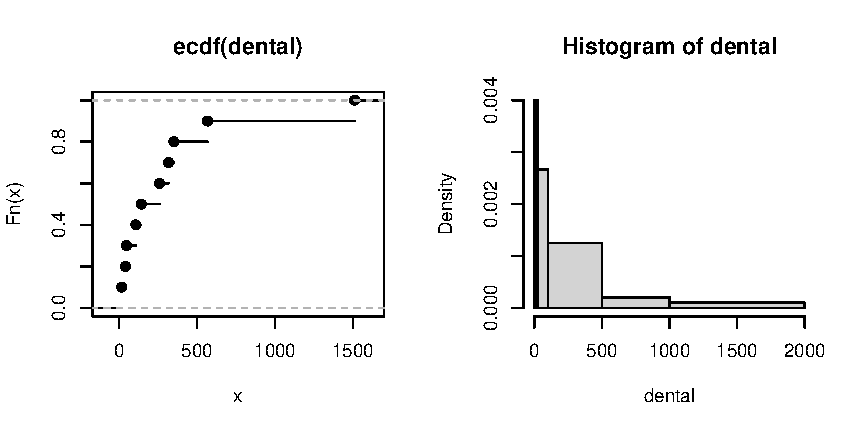
\includegraphics{cjs-rcs-figure}
%   \caption{\ifenglish A sample figure\else Exemple de figure\fi}
%   \label{fig:authguide:sample-figure}
% \end{figure}
%
% \ifenglish%
% If a figure requires an external file, you must provide it with your
% final version, usually in EPS, PDF or PNG format: see %
% \else%
% Si une figure requiert un fichier externe, vous devrez le fournir
% avec votre version finale, habituellement en format EPS, PDF ou PNG;
% consultez les %
% \fi
% \href{https://authorservices.wiley.com/author-resources/Journal-Authors/Prepare/manuscript-preparation-guidelines.html/figure-preparation.html}{%
%   \ifenglish Wiley's guidelines for the preparation of figures\relax
%   \else directives de Wiley pour la préparation des figures\fi}. %
%
% \ifenglish%
% Prepare tables as follows\relax%
% \else%
% Composez vos tableaux selon les règles suivantes\relax%
% \fi
% \footnote{%
%   \ifenglish%
%   These guidelines are adapted from the documentation of %
%   \else%
%   Ces règles sont adaptées de la documentation de %
%   \fi
%   \href{https://ctan.org/pkg/booktabs}{\pkg{booktabs}}.}: %
% \begin{itemize}
% \item %
%   \ifenglish%
%   no vertical lines; %
%   \else%
%   aucun filet vertical; %
%   \fi
% \item %
%   \ifenglish%
%   \cmdprint{\toprule} at the top; %
%   \else%
%   \cmdprint{\toprule} au début; %
%   \fi
% \item %
%   \ifenglish%
%   \cmdprint{\midrule} between the heading and body; %
%   \else%
%   \cmdprint{\midrule} entre l'entête et le corps; %
%   \fi
% \item%
%   \ifenglish%
%   \cmdprint{\bottomrule} at the bottom; %
%   \else%
%   \cmdprint{\bottomrule} au pied; %
%   \fi
% \item %
%   \ifenglish%
%   consistent number of decimal places thoughout the table; %
%   \else%
%   nombre de décimales uniforme; %
%   \fi
% \item %
%   \ifenglish%
%   leading digit in front of a decimal point ($0.1$, not $.1$).
%   \else%
%   marqueur des entiers devant les nombres décimaux ($0,1$ plutôt que
%   $,1$). %
%   \fi
% \end{itemize}
%
% \ifenglish%
% For table footnotes, use the package %
% \else%
% Pour les notes de contenu dans un tableau, utilisez %
% \fi%
% \href{https://ctan.org/pkg/threeparttable}{\pkg{threeparttable}}. %
% \ifenglish%
% However, place \cmdprint{\caption} \emph{outside} the environment
% \code{threeparttable} so that the caption can span the whole width
% of the page: %
% \else%
% Cependant, veillez à placer \cmdprint{\caption} à l'\emph{extérieur}
% de l'environnement \code{threeparttable} afin que la légende occupe
% toute la largeur de la page, le cas échéant: %
% \fi
% \iffalse
%<*example>
% \fi
  \def\CAPTION{\ifenglish caption\else légende\fi}
  \def\LABEL{\ifenglish label\else étiquette\fi}
  \def\TABLECONTENTS{\ifenglish table contents\else contenu du tableau\fi}
\begin{lstlisting}
\begin{table}
  \caption`\marg{\CAPTION}'
  \label`\marg{\LABEL}'
  \centering
  \begin{threeparttable}
    \begin{tabular}`\marg{cols}'
      `\meta{\TABLECONTENTS}'
    \end{tabular}
    \begin{tablenotes}
      `\meta{notes}'
    \end{tablenotes}
  \end{threeparttable}
\end{table}
\end{lstlisting}
% \iffalse
%</example>
% \fi
%
% \ifenglish%
% \section{Computer code and software}
% \else%
% \section{Code informatique et logiciels}
% \fi
% \label{sec:authguide:software}
%
% \ifenglish%
% Providing your computer code is a great way to increase the
% visibility of your work and its accessibility to end users of
% statistics. We strongly encourage that you share your code through a
% suitable repository, such as
% \else%
% Vous améliorerez la visibilité de vos travaux et leur dissémination
% parmi les utilisateurs de la statistique si vous fournissez votre
% code informatique. Nous vous encourageons fortement à partager
% celui-ci par le biais d'un dépôt ouvert, tel que %
% \fi
% \href{https://github.com/}{GitHub}
% \ifenglish or \else ou \fi %
% \href{https://gitlab.com/}{GitLab},
% \ifenglish%
% so that you can keep it up-to-date after the article has been
% published. Alternatively, you may provide your code in the
% Supplementary Material.
% \else%
% afin d'en permettre la mise à jour après la publication de
% l'article. Autrement, vous pouvez inclure le code dans le matériel
% additionnel. %
% \fi
%
% \ifenglish%
% The class does not offer any special features to typeset computer
% code. We recommend that you use specialized packages such
% as %
% \else%
% La classe ne propose aucune fonctionnalité particulière pour la
% présentation du code informatique. Nous vous recommandons d'avoir
% recours à des paquetages spécialisés comme %
% \fi
% \href{https://ctan.org/pkg/fancyvrb}{\pkg{fancyvrb}} %
% \ifenglish or \else ou \fi%
% \href{https://ctan.org/pkg/listings}{\pkg{listings}}. %
% \ifenglish%
% If you use {\Rlang} for your analysis, you could prepare the file
% using a literate programming system such as %
% \else%
% Si vous utilisez {\Rlang} pour effectuer votre analyse, vous pouvez
% rédiger l'article avec un système de programmation lettrée comme %
% \fi
% \href{https://en.wikipedia.org/wiki/Sweave}{Sweave} %
% \ifenglish or \else ou \fi%
% \href{https://en.wikipedia.org/wiki/Knitr}{knitr}.
%
% \ifenglish%
% That said, the class defines a few commands to ease and standardize
% the display of software names and code chunks. The command
% \cmd{\proglang} typesets the names of programming languages and
% software, and there are shortcuts for the most common cases; see
% \autoref{tab:authguide:proglang}. For example, refer to {\Rlang}
% using either \cmdprint{\proglang}\code{\{R\}} or
% \cmdprint{\Rlang}. The command \cmd{\pkg} typesets the names of
% software packages or modules. For example, refer to the {\Rlang}
% package \pkg{copula} using \cmdprint{\pkg}\code{\{copula\}}. %
% \else%
% Cela dit, la classe fournit quelques commandes pour faciliter et
% uniformiser la présentation des noms de logiciels et des extraits de
% code. La commande \cmd{\proglang} compose le nom des langages de
% programmation et des logiciels. Des raccourcis sont fournis pour les
% cas les plus usuels; voir le \autoref{tab:authguide:proglang}.
% Ainsi, pour mentionner {\Rlang}, utilisez
% \cmdprint{\proglang}\code{\{R\}} ou \cmdprint{\Rlang}. La commande
% \cmd{\pkg} compose le nom des paquetages ou modules logiciels. Par
% exemple, vous saisirez \cmdprint{\pkg}\code{\{copula\}} pour
% mentionner le paquetage {\Rlang} \pkg{copula}. %
% \fi
%
% \begin{table}
%   \ifenglish%
%   \caption{List of shortcuts for the names of programming languages
%   and software.}
%   \else%
%   \caption{Liste des raccourcis pour les noms de langages de
%   programmation et de logiciels}
%   \fi
%   \label{tab:authguide:proglang}
%   \centering
%   \begin{tabular}{ll}
%     \toprule
%     \ifenglish Software\else Logiciel\fi & \ifenglish Command\else Commande\fi \\
%     \midrule
%     \Rlang     & \cmd{\Rlang} \\
%     \SASlang   & \cmd{\SASlang} \\
%     \SPSSlang  & \cmd{\SPSSlang} \\
%     \Statalang & \cmd{\Statalang} \\
%     \Pylang    & \cmd{\Pylang} \\
%     \Julialang & \cmd{\Julialang} \\
%     \Clang     & \cmd{\Clang} \\
%     \Cpplang   & \cmd{\Cpplang} \\
%     \bottomrule
%   \end{tabular}
% \end{table}
%
% \ifenglish%
% For small chunks of code, such as the names of exploratory variables
% in a regression model, \cmd{\code} may be useful: it allows you to
% use the characters \code{_}, \code{~} and \code{$} directly. For
% example, you may write \cmdprint{\code}\code{\{patient_age\}} to get
% \code{patient_age}. %
% \else%
% La commande \cmd{\code} est utile pour composer de courts extraits
% de code, comme les noms des variables d'un modèle de régression. La
% commande permet d'utiliser directement les caractères «\code{_}»,
% «\code{~}» et «\code{$}». Par exemple, vous pouvez entrer
% \cmdprint{\code}\code{\{patient_age\}} pour obtenir
% \code{patient_age}. %
% \fi
%
% \ifenglish%
% Remember to report the software packages you used and their
% version numbers; see the following section. %
% \else%
% Vous devez toujours mentionner les logiciels utilisés, ainsi que
% leur version. La section suivante fournit plus de détails à ce
% sujet.
% \fi
%
% \ifenglish%
% \section{Citations and references}
% \else%
% \section{Citations et références}
% \fi
% \label{sec:authguide:references}
%
% \ifenglish%
% For citations and references, use {\BibTeX}. Recall that %
% \else%
% Utilisez {\BibTeX} pour les citations et les références. Tel que
% mentionné précédemment, le paquetage %
% \fi%
% \href{https://ctan.org/pkg/natbib}{\pkg{natbib}} %
% \ifenglish%
% is loaded automatically. Please use the \cmd{\citet} and
% \cmd{\citep} commands of \pkg{natbib}.
% \else%
% est chargé automatiquement par la classe. Assurez-vous
% d'utiliser ses commandes \cmd{\citet} et \cmd{\citep}. %
% \fi
%
% \ifenglish%
% The class also uses its own bibliography styles. These styles
% support the standard {\BibTeX} entry types %
% \else%
% La classe a également recours à ses propres styles de bibliographie.
% Ceux-ci prennent en charge les types d'entrées standards de
% {\BibTeX} %
% \fi
% (\code{article}, \code{book}, \code{proceedings}, etc.) %
% \ifenglish%
% and the standard fields %
% \else%
% et les champs standards %
% \fi%
% (\code{author}, \code{title}, \code{journal}, etc.). %
% \ifenglish%
% Furthermore, the styles support %
% \else%
% De plus, ils ajoutent les champs %
% \fi%
% \code{doi}, \code{isbn}, \code{url} \ifenglish and \else et \fi
% \code{language}.
% \ifenglish%
% These are explained in the examples below. %
% \else%
% Les exemples ci-dessous illustrent chacun de ces champs. %
% \fi%
%
% \begin{itemize}
% \item %
%   \ifenglish%
%   Articles with one author: \citet{Genest:1999}. To include a
%   DOI, use the field \code{doi} with a value in the format
%   \meta{prefix}\code{/}\meta{suffix} (for example,
%   \code{10.2307/3315650}). A hyperlink to the resource is then
%   created automatically. Note that journal names should not be
%   abbreviated. %
%   \else%
%   Articles avec un auteur unique: \citet{Genest:1999}. Pour ajouter
%   un identificateur DOI, utilisez le champ \code{doi} avec une valeur
%   de la forme \meta{préfixe}\code{/}\meta{suffixe} (par exemple:
%   \code{10.2307/3315650}). Un hyperlien vers la ressource est créé
%   automatiquement. Inscrivez les noms des journaux au long. %
%   \fi
% \item %
%   \ifenglish%
%   Articles with two authors: \citet{Qin/Lawless:1995}. Articles
%   with three or more authors: \citet{Davison/Fraser/Reid:2006} or
%   \citet{Granville:2023}. For articles with more than ten authors
%   \citep[such as][]{Teufel:2016}, give the first seven names
%   followed by ``and others''. {\BibTeX} will replace this by
%   ``et~al.''
%   \else%
%   Articles avec deux auteurs: \citet{Qin/Lawless:1995}. Articles
%   avec trois auteurs ou plus: \citet{Davison/Fraser/Reid:2006} ou
%   encore \citet{Granville:2023}. Pour les articles comptant plus de
%   dix auteurs \citep[par exemple:][]{Teufel:2016}, inscrivez les
%   noms des sept premiers auteurs, suivis de \emph{and others}.
%   {\BibTeX} inscrira automatiquement «et collab.» dans la notice.
%   \fi
% \item %
%   \ifenglish%
%   Use the field \code{language} for foreign-language articles, as in
%   \citet{Hoeffding:1940} (German) or
%   \citet{Ghoudi/Khoudraji/Rivest:1998} (French). Including this
%   information in the {\BibTeX} entry ensures that the title words
%   are hyphenated according to the rules of the corresponding
%   language. %
%   \else%
%   Le champ \code{language} permet d'indiquer la langue d'une notice
%   lorsqu'elle diffère de celle de l'article. C'est important pour la
%   coupure de mots dans les titres. Par exemple, pour le présent
%   document en français, la plupart des entrées de la bibliographie
%   déclarent l'anglais comme langue, alors que \citet{Hoeffding:1940}
%   déclare l'allemand. En revanche,
%   \citet{Ghoudi/Khoudraji/Rivest:1998} déclare le français pour la
%   version anglaise du document. %
%   \fi
% \item %
%   \ifenglish%
%   Books and other formats use the same author rules as articles.
%   An example of a book with two authors is
%   \citet{Kalbfleisch/Prentice:2002}. You may use \code{isbn} to include
%   the book's ISBN. Include the relevant page, section, or chapter
%   whenever possible in \cmd{\citet} and \cmd{\citep}. For example,
%   partial likelihood estimation in the Cox regression model may be
%   found in %
%   \else%
%   Les règles pour les auteurs de livres et autres types d'entrées
%   sont les mêmes que pour les articles.
%   \citet{Kalbfleisch/Prentice:2002} est un exemple de livre comptant
%   deux auteurs. Utilisez le champ \code{isbn} pour préciser le
%   numéro ISBN de l'ouvrage. Quand vous citez un livre, précisez
%   autant que faire se peut la page, la section ou le chapitre dans
%   les commandes \cmd{\citet} et \cmd{\citep}. Par exemple,
%   l'estimation par vraisemblance partielle dans le modèle de
%   régression de Cox est traitée dans %
%   \fi
%   \citet[\ifenglish Section\else section\fi~4.2]{Kalbfleisch/Prentice:2002}; %
%   \ifenglish see also \else voir aussi \fi %
%   \citet[\ifenglish Chapter\else chapitre\fi~6]{Kalbfleisch/Prentice:2002}.
% \item %
%   \ifenglish%
%   For references to articles in an edited book, include the page
%   numbers of the article, as well as the names of the book's
%   editors, such as \citet{Roberts:2009}. Again, we encourage you to
%   include the DOI. %
%   \else%
%   Pour la notice d'une partie d'un ouvrage collectif, précisez les
%   pages de la partie citée ainsi que les noms des éditeurs, tel que
%   dans \citet{Roberts:2009}. Ici aussi, nous vous invitons à inclure
%   un identificateur DOI. %
%   \fi
% \item %
%   \ifenglish%
%   You may need to cite a PhD thesis such as \citet{Syed:2022} or a
%   technical report such as \citet{Haas:2001} or an unpublished
%   manuscript posted on arXiv such as \citet{Tang/Kong/Wang:2023}.
%   If you have a DOI or URL, include it in the entry using \code{doi}
%   or \code{url}. If both are present in the database, the DOI
%   takes precedence.
%   \else%
%   Vous pouvez citer une thèse de doctorat \citep{Syed:2022}, un
%   rapport technique \citep{Haas:2001} ou une publication
%   préliminaire dans arXiv \citep{Tang/Kong/Wang:2023}. Saisissez les
%   identificateur DOI et les adresses URL avec les champs \code{doi}
%   et \code{url}. Lorsque les deux sont présents dans la base de
%   données, l'identificateur DOI a priorité. %
%   \fi
% \item %
%   \ifenglish%
%   Cite the software you used in your statistical analysis,
%   especially Free Software. To cite {\Rlang}, use the {\BibTeX}
%   entry provided by the command %
%   \else%
%   Citez les logiciels utilisés pour vos analyses statistiques, tout
%   particulièrement les logiciels libres. Pour citer {\Rlang},
%   utilisez l'entrée {\BibTeX} produite par la commande %
%   \fi
% \iffalse
%<*example>
% \fi
\begin{lstlisting}
> citation()
\end{lstlisting}
% \iffalse
%</example>
% \fi
%   \ifenglish%
%   Don't forget to include the version of {\Rlang}, as in:
%   ``Computations in this article were performed using {\Rlang}
%   \citep[v4.5.0]{Rlang}''. You can get this via:
%   \else%
%   N'oubliez pas d'inclure aussi la version de {\Rlang} dans une
%   mention de la forme «Les calculs de cet article ont été effectués
%   avec {\Rlang} \citep[v4.5.0]{Rlang}». L'expression {\Rlang}
%   suivante fournit la version du logiciel: %
%   \fi
% \iffalse
%<*example>
% \fi
\begin{lstlisting}
> R.version.string
\end{lstlisting}
% \iffalse
%</example>
% \fi
%   \ifenglish%
%   To cite an {\Rlang} package, use the command \code{citation} with
%   the name of the package in argument, e.g.\ %
%   \else%
%   Pour citer un paquetage {\Rlang}, utilisez aussi la commande
%   \code{citation}, mais en ajoutant le nom du paquetage en
%   argument: %
%   \fi
% \iffalse
%<*example>
% \fi
\begin{lstlisting}
> citation("copula")
\end{lstlisting}
% \iffalse
%</example>
% \fi
%   \ifenglish%
%   This specific example asks you to cite three articles
%   \citep{Yan:2007,Kojadinovic/Yan:2010,Hofert/Maechler:2011} as well
%   as the software itself \citep{Rcopula:2024}.
%   \else%
%   Dans cet exemple en particulier, on demande de citer trois
%   articles
%   \citep{Yan:2007,Kojadinovic/Yan:2010,Hofert/Maechler:2011} en plus
%   du logiciel lui-même \citep{Rcopula:2024}. %
%   \fi
% \item %
%   \ifenglish%
%   To cite data, please review %
%   \else%
%   Si vous devez citer des données, consultez la %
%   \fi
%   \href{https://authorservices.wiley.com/author-resources/Journal-Authors/open-access/data-sharing-citation/data-citation-policy.html}{%
%     \ifenglish Wiley's data citation policy\relax
%     \else politique de citation des données de Wiley\fi}. %
%   \ifenglish%
%   An example of a data citation is \citet{StatCan:2023}.
%   \else%
%   Un exemple de citation de données est \citet{StatCan:2023-fr}.
%   \fi
% \item %
%   \ifenglish%
%   You can also cite a webpage, for example \citet{Wolfram:2010}.
%   Include the date of access using the \code{note} field. %
%   \else%
%   Vous pouvez citer une page web, par exemple \citet{Wolfram:2010}.
%   Précisez la date de consultation de la page dans le champ
%   \code{note}. %
%   \fi
% \end{itemize}
%
% \appendix
%
% \ifenglish%
% \section{Proofs}
% \else%
% \section{Démonstrations}
% \fi
% \label{sec:authguide:proofs}
%
% \ifenglish%
% Appendices usually present original proofs or longer mathematical
% derivations; don't forget to cite them in the main article. You
% may structure each appendix into multiple sections and
% subsections. %
% \else%
% Les annexes sont habituellement réservées aux démonstrations ou
% longs développements mathématiques. Vous devez les citer dans le
% corps de l'article. Vous pouvez diviser les annexes en sections et
% sous-sections. %
% \fi
%
% \ifenglish%
% \section{Supplementary material}
% \else%
% \section{Matériel additionnel}
% \fi
% \label{sec:authguide:supplement}
%
% \ifenglish%
% To make your article accessible to a wide readership and to control
% its length, consider providing online supplementary material, citing
% it in the main article. It may contain additional simulation
% results, lengthy tables or figures, auxiliary results, proofs that
% are direct adaptations of calculations already published elsewhere,
% details about the code and software implementation, and so on. That
% said, we encourage you to place original mathematical proofs in an
% appendix and to present the ideas behind these proofs in the main
% text. %
% \else%
% Le matériel additionnel rendu disponible en ligne permet d'élargir
% le lectorat de votre article tout en limitant sa longueur. Vous
% devez citer le matériel additionnel dans l'article. Celui-ci peut
% contenir, entre autres, des résultats de simulation additionnels, de
% longs tableaux ou de grandes figures, des résultats auxiliaires, des
% démonstrations qui sont des applications directes de résultats déjà
% publiés ailleurs, des détails à propos de la mise en œuvre
% informatique. Attention, toutefois: les démonstrations originales
% sont mieux à leur place dans une annexe. Présentez simplement les
% idées fortes derrière celles-ci dans le corps du texte. %
% \fi
%
% \ifenglish%
% To prepare the supplementary material, use the option
% \code{supplement}: %
% \else%
% Pour préparer le matériel additionnel, utilisez l'option
% \code{supplement} de la classe: %
% \fi
% \iffalse
%<*example>
% \fi
\begin{lstlisting}
\documentclass[`\LANGOPT',supplement]{cjs-rcs-article}
\end{lstlisting}
% \iffalse
%</example>
% \fi
% \ifenglish%
% or, to make the supplement suitable for review, %
% \else%
% ou, pour anonymiser le matériel additionnel en vue de l'évaluation
% par les pairs,
% \fi
% \iffalse
%<*example>
% \fi
\begin{lstlisting}
\documentclass[`\LANGOPT',supplement,review]{cjs-rcs-article}
\end{lstlisting}
% \iffalse
%</example>
% \fi
% \ifenglish%
% Your supplementary material is published as supplied, and a proof is
% not made available, so be sure to double-check the file and to
% provide the material in its final format. %
% \else%
% Nous publions votre matériel additionnel tel quel; aucune épreuve ne
% vous sera fournie. Assurez-vous donc de la conformité de votre
% fichier. %
% \fi
%
% \vspace*{10pt}
% \hfill
% \ifenglish%
%   \emph{Have fun writing!}
% \else%
%   \emph{Bonne rédaction!}
% \fi%
%
% \begin{thebibliography}{23}
% \providecommand{\natexlab}[1]{#1}
% \providecommand{\url}[1]{\texttt{#1}}
% \providecommand{\urlprefix}{}
% \providecommand{\doiprefix}{doi: }
% \expandafter\ifx\csname href\endcsname\relax
%   \providecommand{\urldoi}[1]{#1}\else
%   \providecommand{\urldoi}[1]{\href{https://doi.org/#1}{#1}}\fi
% \providecommand{\selectlanguage}[1]{\relax}
% 
% \bibitem[{Davison et~al.(2006)Davison, Fraser, and
%   Reid}]{Davison/Fraser/Reid:2006}
% Davison, A.~C., Fraser, D. A.~S., and Reid, N. (2006).
% \newblock {\selectlanguage{english}Improved likelihood inference for discrete
%   data}.
% \newblock \emph{Journal of the Royal Statistical Society Series B: Statistical
%   Methodology}, 68(3):495--508.
% \newblock \doiprefix\urldoi{10.1111/j.1467-9868.2006.00548.x}.
% 
% \bibitem[{Downes and Beeton(2017)}]{Downes:short-math-guide:2017}
% Downes, M. and Beeton, B. (2017).
% \newblock {\selectlanguage{english}\emph{Short Math Guide for {\LaTeX}}}.
% \newblock American Mathematical Society.
% \newblock \urlprefix\url{https://ctan.org/pkg/short-math-guide}.
% 
% \bibitem[{Genest(1999)}]{Genest:1999}
% Genest, C. (1999).
% \newblock {\selectlanguage{english}Probability and statistics: A tale of two
%   worlds?}
% \newblock \emph{The Canadian Journal of Statistics}, 27(2):421--444.
% \newblock \doiprefix\urldoi{10.2307/3315650}.
% 
% \bibitem[{Ghoudi et~al.(1998)Ghoudi, Khoudraji, and
%   Rivest}]{Ghoudi/Khoudraji/Rivest:1998}
% Ghoudi, K., Khoudraji, A., and Rivest, L.-P. (1998).
% \newblock {\selectlanguage{french}Propri\'et\'es statistiques des copules de
%   valeurs extr\^emes bidimensionnelles}.
% \newblock \emph{The Canadian Journal of Statistics}, 26:187--197.
% \newblock \doiprefix\urldoi{10.2307/3315683}.
% 
% \bibitem[{Granville et~al.(2023)Granville, Woolford, Dean, Boychuk, and
%   McFayden}]{Granville:2023}
% Granville, K., Woolford, D.~G., Dean, C.~B., Boychuk, D., and McFayden, C.~B.
%   (2023).
% \newblock {\selectlanguage{english}On the selection of an interpolation method
%   with an application to the {F}ire {W}eather {I}ndex in {O}ntario, {C}anada}.
% \newblock \emph{Environmetrics}, 34(2):e2758.
% \newblock \doiprefix\urldoi{10.1002/env.2758}.
% 
% \bibitem[{Haas(2001)}]{Haas:2001}
% Haas, M. (2001).
% \newblock {\selectlanguage{english}\emph{New Methods in Backtesting}}.
% \newblock Tech. rep., Financial Engineering Research Center, Bonn, Germany.
% \newblock \urlprefix\url{https://www.yumpu.com/s/L9EC3aHSgRvWa763}.
% 
% \bibitem[{Higham(2020)}]{Higham:2020}
% Higham, N.~J. (2020).
% \newblock {\selectlanguage{english}\emph{Handbook of Writing for the
%   Mathematical Sciences}}.
% \newblock 3rd ed. SIAM, Philadelphia.
% \newblock ISBN 978-1-61197-609-0.
% \newblock \doiprefix\urldoi{10.1137/1.9781611976106}.
% 
% \bibitem[{Hoeffding(1940)}]{Hoeffding:1940}
% Hoeffding, W. (1940).
% \newblock {\selectlanguage{german}Ma{\ss}stabinvariante {K}orrelationstheorie
%   f\"ur diskontinuierliche {V}erteilungen}.
% \newblock \emph{Archiv f\"ur mathematische Wirtschafts- und Sozialforschung},
%   7:4--70.
% 
% \bibitem[{Hofert et~al.(2023)Hofert, Kojadinovic, Maechler, and
%   Yan}]{Rcopula:2024}
% Hofert, M., Kojadinovic, I., Maechler, M., and Yan, J. (2023).
% \newblock {\selectlanguage{english}\emph{copula: Multivariate Dependence with
%   Copulas}}.
% \newblock \urlprefix\url{https://cran.r-project.org/package=copula}.
% \newblock R package version 1.1-4.
% 
% \bibitem[{Hofert and M\"achler(2011)}]{Hofert/Maechler:2011}
% Hofert, M. and M\"achler, M. (2011).
% \newblock {\selectlanguage{english}Nested {A}rchimedean copulas meet {R}: The
%   {nacopula} package}.
% \newblock \emph{Journal of Statistical Software}, 39(9):1--20.
% \newblock \doiprefix\urldoi{10.18637/jss.v039.i09}.
% 
% \bibitem[{Kalbfleisch and Prentice(2002)}]{Kalbfleisch/Prentice:2002}
% Kalbfleisch, J.~D. and Prentice, R.~L. (2002).
% \newblock {\selectlanguage{english}\emph{The Statistical Analysis of Failure
%   Time Data}}.
% \newblock 2nd ed. Wiley Series in Probability and Statistics,
%   Wiley-Interscience [John Wiley \& Sons], Hoboken, NJ.
% \newblock ISBN 9780471363576.
% \newblock \doiprefix\urldoi{10.1002/9781118032985}.
% 
% \bibitem[{Kojadinovic and Yan(2010)}]{Kojadinovic/Yan:2010}
% Kojadinovic, I. and Yan, J. (2010).
% \newblock {\selectlanguage{english}Modeling multivariate distributions with
%   continuous margins using the {copula} {R} package}.
% \newblock \emph{Journal of Statistical Software}, 34(9):1--20.
% \newblock \doiprefix\urldoi{10.18637/jss.v034.i09}.
% 
% \bibitem[{Mermin(1989)}]{Mermin:1989}
% Mermin, N.~D. (1989).
% \newblock {\selectlanguage{english}What's wrong with these equations?}
% \newblock \emph{Physics Today}, 42(10):9--11.
% \newblock \doiprefix\urldoi{10.1063/1.2811173}.
% 
% \bibitem[{Oetiker et~al.(2021)Oetiker, Partl, Hyna, and
%   Schlegl}]{Oetiker:lshort-english:2021}
% Oetiker, T., Partl, H., Hyna, I., and Schlegl, E. (2021).
% \newblock {\selectlanguage{english}\emph{The Not So Short Introduction to
%   {\LaTeXe}}}.
% \newblock \urlprefix\url{https://ctan.org/pkg/lshort-english}.
% \newblock Version 6.4.
% 
% \bibitem[{Qin and Lawless(1995)}]{Qin/Lawless:1995}
% Qin, J. and Lawless, J. (1995).
% \newblock {\selectlanguage{english}Estimating equations, empirical likelihood
%   and constraints on parameters}.
% \newblock \emph{The Canadian Journal of Statistics}, 23(2):145--159.
% \newblock \doiprefix\urldoi{10.2307/3315441}.
% 
% \bibitem[{{R Core Team}(2024)}]{Rlang}
% {R Core Team} (2024).
% \newblock {\selectlanguage{english}\emph{R: A Language and Environment for
%   Statistical Computing}}.
% \newblock R Foundation for Statistical Computing, Vienna, Austria.
% \newblock \urlprefix\url{https://www.r-project.org/}.
% 
% \bibitem[{Roberts et~al.(2009)Roberts, Ren, and Rao}]{Roberts:2009}
% Roberts, G., Ren, Q., and Rao, J. N.~K. (2009).
% \newblock {\selectlanguage{english}Using marginal mean models for data from
%   longitudinal surveys with a complex design: Some advances in methods}.
% \newblock In R.~Lynn, editor, \emph{Methodology of Longitudinal Surveys}, pages
%   351--366. John Wiley \& Sons, New York.
% \newblock ISBN 9780470018712.
% \newblock \doiprefix\urldoi{10.1002/9780470743874}.
% 
% \bibitem[{{Statistics Canada}(2023)}]{StatCan:2023}
% {Statistics Canada} (2023).
% \newblock {\selectlanguage{english}Table 13-10-0096-01 {H}ealth
%   characteristics, annual estimates, inactive}.
% \newblock \doiprefix\urldoi{10.25318/1310009601-eng}.
% 
% \bibitem[{Syed(2022)}]{Syed:2022}
% Syed, S. (2022).
% \newblock {\selectlanguage{english}\emph{Non-reversible parallel tempering on
%   optimized paths}}.
% \newblock Ph.D. thesis, University of British Columbia, Vancouver (BC), Canada.
% \newblock \doiprefix\urldoi{10.14288/1.0413120}.
% 
% \bibitem[{Tang et~al.(2023)Tang, Kong, and Wang}]{Tang/Kong/Wang:2023}
% Tang, D., Kong, D., and Wang, L. (2023).
% \newblock {\selectlanguage{english}The synthetic instrument: From sparse
%   association to sparse causation}.
% \newblock arXiv.
% \newblock \doiprefix\urldoi{10.48550/arXiv.2304.01098}.
% 
% \bibitem[{Teufel et~al.(2016)Teufel, Diro, Whan, Milrad, Jeong, Ganji, Huziy
%   et~al.}]{Teufel:2016}
% Teufel, B., Diro, G.~T., Whan, K., Milrad, S.~M., Jeong, D.~I., Ganji, A.,
%   Huziy, O. et~al. (2016).
% \newblock {\selectlanguage{english}Investigation of the 2013 {A}lberta flood
%   from a weather/climate perspective}.
% \newblock \emph{Climate Dynamics}, 48(9):2881--2899.
% \newblock \doiprefix\urldoi{10.1007/s00382-016-3239-8}.
% 
% \bibitem[{{W}olfram {R}esearch(2010)}]{Wolfram:2010}
% {W}olfram {R}esearch (2010).
% \newblock {\selectlanguage{english}Pearson distribution}.
% \newblock
%   \urlprefix\url{https://reference.wolfram.com/language/ref/PearsonDistribution.html}.
% \newblock Accessed October 12, 2022.
% 
% \bibitem[{Yan(2007)}]{Yan:2007}
% Yan, J. (2007).
% \newblock {\selectlanguage{english}Enjoy the joy of copulas: With a package
%   copula}.
% \newblock \emph{Journal of Statistical Software}, 21(4):1--21.
% \newblock \doiprefix\urldoi{10.18637/jss.v021.i04}.
% 
% \end{thebibliography}
%
% \ifenglish%
%   \PrintChanges
% \else%
%   \section*{Historique des versions}
%   \label{sec:authguide:implementation}
%   Consultez la version anglaise de ce document pour l'historique des
%   versions. %
% \fi

%</fr-doc>
% \fi
% \GetFileInfo{cjs-rcs-authguide.dtx}
% \expandafter\parsedate\filedate\relax
%
% \changes{2.0}{2026-03-05}{Adapt the guidelines to the single-blind
% review process.}
% \changes{1.3}{2025-08-29}{Improve the French version in a few
% places.}
% \changes{1.2c}{2025-08-11}{Add guidelines on the length and contents
% of the abstracts.}
% \changes{1.2b}{2025-07-25}{Fix the link to instructions on updating
% a {\TeX} distribution.}
% \changes{1.2b}{2025-07-25}{Improve the text of the French version in
% a few places and fix typos.}
% \changes{1.2b}{2025-07-25}{Use the French variant of the reference
% Statistics Canada (2023) in the French version.}
% \changes{1.2a}{2025-07-24}{Fix the typesetting of a few entries in
% the list of references.}
% \changes{1.2a}{2025-07-24}{Provide more specific URLs for Oetiker et
% al. (2021) and Oetiker et collab. (2011).}
% \changes{1.2}{2025-07-10}{Initial version in the distribution.}
%
% \ifenglish%
% \makeatletter
% \title[Author guidelines for \CJS@journalname@en]{%
% Author guidelines \\ for \TheCJS}
% \makeatother
% \author{\SSCen}
% \affil{Guidelines developed by Julie Falkner, Vincent Goulet,
% Johanna Nešlehová}
% \runningauthor{Statistical Society of Canada}
% \else%
% \makeatletter
% \title[Directives pour les auteurs de \CJS@journalname@fr]{%
%   Directives pour les auteurs \\ de \LaRevue}
% \makeatother
% \author{\SSCfr}
% \affil{Directives rédigées par Julie Falkner, Vincent Goulet,
% Johanna Nešlehová}
% \runningauthor{Société canadienne de statistique}
% \fi
%
% \begin{englishabstract}
%   This guide provides the stylistic and presentation guidelines
%   for authors submitting an article to {\TheCJS}. Although the
%   guidelines apply broadly, the document assumes that the
%   manuscript is prepared using {\LaTeX} and the class
%   {\CJSclass}. This guide is also available in%
%   \ifenglish French\else English\fi.
% \end{englishabstract}
% \begin{frenchabstract}
%   Ce guide fournit les directives en matière de style et de
%   présentation pour les auteurs qui soumettent un article dans
%   {\LaRevue}. Les directives s'appliquent de manière générale, mais
%   le document se concentre sur la préparation d'un manuscript avec
%   {\LaTeX} et la classe {\CJSclass}. Ce guide est aussi disponible
%   en \ifenglish français\else anglais\fi.
% \end{frenchabstract}
%
% ^^A abusing the 'classification' environment. The final period is
% ^^A added by the environment.
% \begin{classification}[Version]
% \item[] %
%   \ifenglish%
%   These guidelines accompany the class {\CJSclass}~{\fileversion},
%   dated {\filedate} %
%   \else%
%   Ces directives accompagnent la classe {\CJSclass}~{\fileversion},
%   datée du {\filedate} %
%   \fi
% \end{classification}
%
% \licence{{\ccbysa*} 2025--{\year}, {\SSCen}~{\textbar}~{\SSCfr}}
%
% \makeCJStitle
%
% \section{Introduction}
% \label{sec:authguide:introduction}
%
% \ifenglish%
% This document provides guidelines for authors of {\TheCJS}. Please
% read them carefully: manuscripts that are scientifically acceptable
% but don't follow these stylistic guidelines will need additional
% work by the editors and copy-editors, delaying publication. %
% \else%
% Le présent document fournit les directives aux auteurs de
% {\LaRevue}. Lisez-le avec attention, car un manuscript
% scientifiquement acceptable verra sa publication retardée par le
% travail d'édition additionnel requis s'il ne respecte pas les
% directives en matière de style. %
% \fi
%
% \ifenglish%
% Manuscripts may be submitted in either English or French. We accept
% submissions in Microsoft~Word, but authors are encouraged to use
% {\LaTeX} and the class {\CJSclass}, described in this guide. You'll
% find documentation and additional information at the %
% \href{\siteurl}{project website}. %
% \else%
% Vous pouvez soumettre votre manuscript en français comme en anglais.
% Bien que nous acceptions le format Microsoft Word, nous recommandons
% d'utiliser {\LaTeX} et la classe {\CJSclass}. C'est d'ailleurs le
% mode de préparation décrit dans le présent guide. Vous trouverez de
% la documentation et des informations additionnelles dans le %
% \href{\siteurl/fr}{site web du projet}. %
% \fi%
%
% \ifenglish%
% Using {\CJSclass} requires an up-to-date {\TeX} distribution, so
% start by %
% \else%
% La classe {\CJSclass} requiert une distribution {\TeX} à jour, alors
% assurez-vous avant toute chose d'en %
% \fi
% \href{https://tex.stackexchange.com/q/55437}{\ifenglish doing this
% update\else effectuer la mise à jour\fi}. %
% \ifenglish%
% Since the class is part of the standard {\TeX} distributions via the
% package {\CJSpkg}, it will also get installed or updated. %
% \else
% Puisque la classe fait partie des distributions {\TeX} standards via
% le paquetage {\CJSpkg}, elle sera de ce fait installée ou mise à
% jour. %
% \fi
%
% \tipbox{%
%   \ifenglish%
%   If you get error messages about missing or outdated packages when
%   using {\CJSclass}, the solution is to update your {\TeX}
%   distribution. %
%   \else%
%   Si vous obtenez des messages d'erreur au sujet de paquetages
%   manquants ou obsolètes en utilisant {\CJSclass}, c'est que vous
%   devez mettre à jour de votre distribution {\TeX}. %
%   \fi}
%
% \ifenglish%
% \section{Preparing your article}
% \else%
% \section{Mise en place de l'article}
% \fi
% \label{sec:authguide:preparing}
%
% \ifenglish%
% Don't start from scratch. The class ships with templates for
% articles in English and French. If you're using the version included
% with your {\TeX} distribution, the templates are located with the
% documentation of the class. You may also obtain them from %
% \else%
% Ne partez pas de zéro. La classe est livrée avec des gabarits pour
% des articles en français et en anglais. Si vous utilisez la version
% fournie avec votre distribution {\TeX}, les gabarits sont classés
% avec la documentation de la classe. Vous pouvez aussi les récupérer
% depuis %
% \fi%
% \href{https://ctan.org/pkg/\CJSname}{CTAN}. %
% \ifenglish%
% Copy the template to your working directory and follow the
% instructions and examples therein. You may also compile the template
% as is, obtaining a complete sample article. %
% \else%
% Copiez le gabarit dans votre dossier de travail et suivez les
% directives et les exemples qui s'y trouvent. Vous pouvez compiler le
% gabarit tel quel pour produire un exemple d'article complet. %
% \fi
%
% \changes{1.3}{2025-08-27}{Instruct, in the introduction of
% \emph{Preparing your article}, to type non-ASCII characters directly
% rather than by using {\TeX} commands.}
% \ifenglish%
% If you need non-ASCII characters (such as accented letters) in your
% manuscript, type them directly instead of using {\TeX} commands
% (e.g.~\code{é} and \code{ü} instead of \code{{\bs}'e} and
% \code{{\bs}"u}), and save your file using %
% \else%
% Si vous avez recours à des caractères non-ASCII (comme des lettres
% accentuées), entrez directement ceux-ci au clavier, sans passer par
% les commandes {\TeX} (par exemple: «\code{é}» et «\code{ü}» plutôt
% que «\code{{\bs}'e}» et «\code{{\bs}"u}»). Enregistrez le fichier
% dans le codage de caractères %
% \fi%
% \href{https://fr.wikipedia.org/wiki/UTF-8}{UTF-8} %
% \ifenglish%
% character encoding. We recommend that you compile with {\LuaLaTeX},
% which allows for modern multilingual typesetting. Various packages
% are available with {\CJSclass} and there's no need to load them
% again: these include %
% \else%
% et compilez avec {\LuaLaTeX} pour tirer pleinement profit des
% caractéristiques de {\CJSclass}. Plusieurs paquetages étant chargés
% par la classe, vous n'avez pas besoin de les charger de nouveau.
% Parmi ceux-ci, mentionnons:%
% \fi
% \pkg{amsmath}, %
% \pkg{amsthm}, %
% \pkg{babel}, %
% \pkg{enumitem}, %
% \pkg{fontawesome5}, %
% \pkg{graphicx}, %
% \pkg{natbib}, %
% \pkg{numprint}, %
% \pkg{relsize}, %
% \pkg{url}\ifenglish, and \else\ et \fi %
% \pkg{xcolor}. %
%
% \ifenglish%
% \subsection{Class declaration}
% \else%
% \subsection{Déclaration de la classe}
% \fi
% \label{sec:authguide:preparing:documentclass}
%
% \ifenglish%
% The class requires the options \code{english} and \code{french}. The
% order is important: the \emph{second} one is the main language.
% Therefore, for an article in English use: %
% \else%
% Vous devez charger la classe avec les options \code{english} et
% \code{french}. Leur ordre est important: la \emph{seconde} est la
% langue principale de l'article. Par conséquent, pour un article en
% français, chargez la classe avec: %
% \fi
% \iffalse
%<*example>
% \fi
\def\LANGOPT{\ifenglish french,english\else english,french\fi}
\begin{lstlisting}
\documentclass[`\LANGOPT']{cjs-rcs-article}
\end{lstlisting}
% \iffalse
%</example>
% \fi%
%
% \ifenglish%
% \subsection{Title page}
% \else%
% \subsection{Page de titre}
% \fi
% \label{sec:authguide:preparing:titling}
%
% \ifenglish%
% Your preamble will contain the following declarations: %
% \else%
% Le préambule de votre manuscript doit contenir les déclarations
% suivantes pour produire les informations de la page de titre. %
% \fi
%
% \begin{itemize}
% \item %
%   \ifenglish%
%   \cmd{\title}: title of the article. See
%   \autoref{sec:authguide:typesetting:titles} for more on titles. Break a
%   long title covering more than one line using using \code{\bs\bs} or
%   \cmdprint{\newline}. If the title doesn't fit in the running head,
%   supply a short title as an optional argument (between square
%   brackets \texttt{[~]}): %
%   \else%
%   \cmd{\title}: titre de l'article; voir la
%   \autoref{sec:authguide:typesetting:titles} pour des détails
%   additionnels sur la composition du titre. Coupez manuellement un
%   titre qui nécessite plus d'une ligne avec \code{\bs\bs} ou
%   \cmdprint{\newline}. Si le titre est trop long pour l'entête,
%   fournissez une version courte en argument optionnel (entre les
%   crochets \texttt{[~]}): %
%   \fi%
%   \iffalse
%<*example>
%   \fi
\def\OPT{\ifenglish Short title\else Titre court\fi}
\def\ARG{\ifenglish Full title\else Titre complet\fi}
\begin{lstlisting}
\title`\oarg{\OPT}\marg{\ARG}'
\end{lstlisting}
%   \iffalse
%</example>
%   \fi
% \item %
%   \ifenglish%
%   \cmd{\author} and \cmd{\affil}: author name, ORCID~iD, email and
%   affiliation (give the country name in the language of the
%   article). The corresponding author is specified by
%   \code{corresponding} and surnames via \cmd{\surname}: %
%   \else%
%   \cmd{\author} et \cmd{\affil}: noms, identifiants ORCID, adresses
%   courriel et affiliations des auteurs (indiquez le nom du pays dans
%   la langue de l'article). Indiquez l'auteur correspondant avec
%   \code{corresponding} et entrez les noms de famille avec
%   \cmd{\surname}: %
%   \fi%
%   \iffalse
%<*example>
%   \fi
\def\EMAIL{\ifenglish email\else courriel\fi}
\def\FORENAME{\ifenglish Forename\else Prénom\fi}
\def\SURNAME{\ifenglish Surname\else Nom\fi}
\def\AFFIL{\ifenglish Department, University, City, Country\else%
  Département, Université, Ville, Pays\fi}
\begin{lstlisting}
\author[orcid=`\meta{id}', email=`\meta{\EMAIL}', corresponding]
       {`\meta{\FORENAME}' \surname`\marg{\SURNAME}'}
\affil`\marg{\AFFIL}'
\end{lstlisting}
%   \iffalse
%</example>
%   \fi
%
%   \ifenglish%
%   To acknowledge the Alzheimer’s Disease Neuroimaging Initiative
%   (ADNI), insert \cmd{\ADNIacknowledgement} after the declarations
%   of the authors and the class will add the required statement on
%   the title page. Similarly, \cmd{\ADMCacknowledgement} acknowledges
%   the Alzheimer’s Disease Metabolomics Consortium (ADMC).%
%   \else%
%   Pour reconnaitre la contribution de l'Alzheimer’s Disease
%   Neuroimaging Initiative (ADNI), insérez la commande
%   \cmd{\ADNIacknowledgement} après les définitions de tous les
%   auteurs. La classe se chargera  d'ajouter la déclaration
%   obligatoire dans la page de titre. De manière analogue, la
%   commande \cmd{\ADMCacknowledgement} reconnait la contribution du
%   Alzheimer’s Disease Metabolomics Consortium (ADMC). %
%   \fi
% \item %
%   \ifenglish%
%   \code{englishabstract} and \code{frenchabstract} environments: the
%   required English and French abstracts. These should be concise;
%   the English abstract must not exceed 20~lines in the format of the
%   class. We strongly discourage symbols, formulas and citations in
%   the abstracts. If you ask us to, we'll prepare a French abstract
%   for your English-language article. The order of these declarations
%   is not important: %
%   \else%
%   environnements \code{frenchabstract} et \code{englishabstract}:
%   résumés français et anglais. Ceux-ci doivent être concis: la
%   version anglaise ne doit pas dépasser 20~lignes dans le format de
%   la classe. Les symboles, formules mathématiques et citations sont
%   fortement déconseillées dans les résumés. Nous vous fournirons sur
%   demande un résumé en anglais pour un article en français. L'ordre
%   des déclarations n'a pas d'importance: %
%   \fi
%   \iffalse
%<*example>
%   \fi
\begin{lstlisting}
\begin{englishabstract}
  `\meta{Text of the English abstract}'
\end{englishabstract}

\begin{frenchabstract}
  `\meta{Texte du résumé en français}'
\end{frenchabstract}
\end{lstlisting}
%   \iffalse
%</example>
%   \fi
% \item %
%   \ifenglish%
%   \code{keywords} environment: the list of keywords. Capitalize
%   only the first keyword, order them alphabetically, and don't include
%   any punctuation: %
%   \else%
%   environnement \code{keywords}: liste de mots-clés. Saisissez les
%   mots-clés en ordre alphabétique, avec une majuscule uniquement
%   pour le premier et sans aucune ponctuation: %
%   \fi%
%   \iffalse
%<*example>
%   \fi
\def\KEYWORDC{\ifenglish Keyword\else Mot-clé\fi}
\def\KEYWORD{\ifenglish keyword\else mot-clé\fi}
\begin{lstlisting}
\begin{keywords}
\item `\normalfont\itshape{\KEYWORDC} 1'
\item `\normalfont\itshape{\KEYWORD} 2'
...
\end{keywords}
\end{lstlisting}
%   \iffalse
%</example>
%   \fi
% \item %
%   \ifenglish%
%   \code{classification} environment: the %
%   \else%
%   environnement \code{classification}: classification mathématique
%   par matières selon le classement %
%   \fi
%   \href{https://msc2020.org}{MSC2020}\ifenglish{ }\else. \fi %
%   \ifenglish%
%   mathematics subject classification. Provide primary and secondary
%   classifications: %
%   \else
%   Indiquez des classifications primaires et secondaires: %
%   \fi
%   \iffalse
%<*example>
%   \fi
\def\PRIMARY{\ifenglish Primary\else Primaire\fi}
\def\SECONDARY{\ifenglish Secondary\else Secondaire\fi}
\def\CODE{\ifenglish code\else rubrique\fi}
\begin{lstlisting}
\begin{classification}
\item[`\PRIMARY'] `\normalfont\itshape{\CODE} 1, {\CODE} 2, \dots'
\item[`\SECONDARY'] `\normalfont\itshape{\CODE} 1, {\CODE} 2, \dots'
\end{classification}
\end{lstlisting}
%   \iffalse
%</example>
%   \fi
% \end{itemize}
%
% \ifenglish%
% \subsection{Back matter}
% \else%
% \subsection{Informations des parties annexes}
% \fi
% \label{sec:authguide:preparing:backmatter}
%
% \ifenglish%
% Articles end with the data sharing statement, acknowledgements,
% etc., and you may also enter these details in the preamble using the
% environments below. Note that ORCID identifiers appear
% automatically. %
% \else%
% Les articles se terminent par des parties annexes contenant les
% conditions de partage des données, les remerciements, etc. Nous vous
% recommandons de saisir ces informations dans le préambule à l'aide
% des environnements ci-dessous. Les identifiants ORCID sont quant à
% eux affichés automatiquement. %
% \fi
%
% \begin{itemize}
% \item %
%   \ifenglish%
%   \code{supplement}: if you have online supplementary
%   material, this is the place to describe it. For example, the
%   Supplementary Material contains auxiliary technical lemmas, a
%   detailed description of the simulation study, and additional
%   simulation results. %
%   \else%
%   \code{supplement}: liste de votre matériel additionnel disponible
%   en ligne, le cas échéant. Le matériel additionnel peut, par exemple,
%   contenir des lemmes techniques supplémentaires, une description
%   détaillée d'une étude de simulation ou des résultats de simulation
%   additionnels. %
%   \fi
% \item %
%   \def\POLICYNAME{\ifenglish Expects Data Sharing\else \emph{Expects Data Sharing}\fi}
%   \ifenglish%
%   \code{sharing}: statement about the availability or absence of
%   shared data. Provide a DOI or URL for the latter, as per our %
%   \else%
%   \code{sharing}: conditions de partage des données de recherche ou
%   explication de leur absence. En vertu de notre politique
%   éditoriale %
%   \fi%
%   \href{https://authorservices.wiley.com/author-resources/Journal-Authors/open-access/data-sharing-citation/data-sharing-policy.html}{\POLICYNAME}\ifenglish{ }\else, \fi %
%   \ifenglish%
%   policy. If there are ethical or legal concerns, we encourage you
%   to provide synthetic data instead. You may also use the
%   environment to describe how to access your code. If data sharing
%   is not applicable, write: ``Data sharing not applicable to this
%   article as no datasets were generated or analyzed during the
%   current study.'' %
%   \else%
%   vous devez fournir un lien permanent vers les données
%   (identificateur DOI ou adresse URL). En cas d'enjeux éthiques ou
%   légaux, utilisez si possible des données de synthèse. Vous pouvez
%   aussi utiliser l'environnement pour indiquer comment accéder à
%   votre code informatique. Si le partage des données ne s'applique
%   pas, écrivez: «Le partage des données ne s'applique pas à cet
%   article car aucun jeu de données n'a été généré au analysé au
%   cours de l'étude.» %
%   \fi
% \item %
%   \ifenglish%
%   \code{acknowledgements}: has a colleague or supervisor provided
%   crucial help or expertise? %
%   \else%
%   \code{acknowledgements}: remerciements, si vous avez obtenu de
%   l'aide cruciale de la part de collègues ou de superviseurs. %
%   \fi%
% \item %
%   \ifenglish%
%   \code{funding}: include your funding information here, and don't
%   abbreviate the names of granting agencies. %
%   \else%
%   \code{funding}: informations sur le financement de la recherche.
%   Indiquez le nom des agences de financement au long. %
%   \fi
% \end{itemize}
%
% \changes{2.0}{2026-02-23}{Section \emph{Anonymous version} becomes
% \emph{Peer review version}, with all anonymity-related material
% deleted.}
% \ifenglish%
% \subsection{Peer review version}
% \else%
% \subsection{Version pour évaluation}
% \fi%
% \label{sec:authguide:preparing:review}
%
% \ifenglish%
% {\TheCJS} uses a single-blind peer review process. Until acceptance,
% please prepare your manuscript using the class option \code{review}
% as follows: %
% \else%
% {\LaRevue} procède à l'évaluation par les pairs en simple anonymat.
% Composez la version de votre manuscrit pour évaluation avec l'option
% \code{review}: %
% \fi%
% \iffalse
%<*example>
% \fi
\begin{lstlisting}
\documentclass[`\LANGOPT',review]{cjs-rcs-article}
\end{lstlisting}
% \iffalse
%</example>
% \fi%
% \changes{1.3}{2025-08-27}{Emphasize in section \emph{Anonymous
% version} that acknowledgements, funding information and ORCID iDs is
% among the information hidden by option \texttt{review}.}
% \ifenglish%
% The option numbers the lines and increases the line spacing. It
% should also be used for your supplementary document; see
% \autoref{sec:authguide:supplement}. After acceptance, remove the
% \code{review} option and compile twice to remove the line numbers. %
% \else%
% L'option numérote les lignes et augmente l'interligne. Vous
% devriez aussi l'utiliser pour le matériel additionnel; voir
% l'\autoref{sec:authguide:supplement}. Une fois votre article accepté
% pour publication, retirez l'option \code{review} et compilez
% au moins deux fois pour annuler l'effet de la numérotation des
% lignes. %
% \fi
%
% \ifenglish%
% Referees and editors may check the literature for overlaps with your
% research. Therefore, provide DOIs, arXiv~IDs, or article numbers in
% the list of references to ease retrieval. If your manuscript is
% based on your thesis, there will be overlap, so ask yourself if you
% really need a reference. Refer to the thesis only if you use
% unpublished results from it that are not included in the current
% manuscript. %
% \else%
% Les arbitres et les éditeurs vérifieront si votre travail recoupe
% des résultats déjà présents dans la littérature. Veillez donc à
% fournir pour vos références des identificateurs DOI ou arXiv,
% ou encore des numéros d'articles, afin d'en faciliter le repérage.
% Les recoupements étant inévitables si l'article est tiré de votre
% thèse, demandez-vous si une référence à celle-ci est vraiment
% nécessaire. Elle ne le sera que si l'article fait appel à des
% résultats de la thèse qui n'ont pas été publiés ailleurs. %
%\fi
%
% \ifenglish%
% We allow submissions of arXiv preprints. %
% \else%
% Vous pouvez soumettre une publication préliminaire arXiv. %
% \fi
%
% \ifenglish%
% \subsection{Repository version}
% \else%
% \subsection{Version préliminaire}
% \fi%
% \label{sec:authguide:preparing:nocjs}
%
% \ifenglish%
% To prepare a version of your article for a repository such as arXiv,
% use the \code{nocjs} option:
% \else%
% Pour créer une version préliminaire de votre article pour
% publication dans une archive ouverte telle que arXiv, utilisez
% l'option \code{nocjs}: %
% \fi%
% \iffalse
%<*example>
% \fi
\begin{lstlisting}
\documentclass[`\LANGOPT',nocjs]{cjs-rcs-article}
\end{lstlisting}
% \iffalse
%</example>
% \fi
%
% \ifenglish%
% \section{Length restrictions}
% \else%
% \section{Longueur maximale}
% \fi
% \label{sec:authguide:length}
%
% \ifenglish%
% Your submission should not exceed 32~pages when compiled with the
% \code{review} option, and this is enforced when a revision is
% invited. It's harder to find reviewers for overly long manuscripts
% and they'll need more time, causing delays throughout the process. %
% \else%
% Votre proposition ne devrait pas excéder 32~pages lorsque composée
% avec l'option \code{review}. Gardez en tête que les longs articles
% compliquent le recrutement d'arbitres et allongent le processus
% de révision, ce qui à terme retarde la publication de votre
% article. %
% \fi
%
% \ifenglish%
% Concise abstracts are preferred. The English version must not
% exceed 20~lines. %
% \else%
% Visez la concision pour vos résumés. La version anglaise ne devrait
% pas dépasser 20~lignes.
% \fi
%
% \ifenglish%
% Lengthy mathematical derivations and proofs are better placed in the
% appendices (see \autoref{sec:authguide:proofs}). Relevant material
% that doesn't belong in the main article can be included in the
% Supplementary Material (see \autoref{sec:authguide:supplement}). %
% \else%
% Les longs développements mathématiques et les longues démontrations
% sont mieux à leur place en annexe (consultez
% l'\autoref{sec:authguide:proofs}). Vous pouvez placer les autres
% éléments utiles, mais non essentiels dans le matériel
% additionnel (voir l'\autoref{sec:authguide:supplement}). %
% \fi
%
% \ifenglish%
% \section{Article structure}
% \else%
% \section{Structure de l'article}
% \fi
% \label{sec:authguide:structure}
%
% \ifenglish%
% Our templates will guide you through the following structure: %
% \else%
% Suivez nos gabarits, ils vous guideront vers la structure suivante: %
% \fi
% \begin{itemize}
% \item %
%   \ifenglish%
%   The title page created with \cmd{\maketitle}. %
%   \else%
%   La page de titre produite avec \cmd{\maketitle}. %
%   \fi
% \item %
%   \ifenglish%
%   The introduction. %
%   \else%
%   L'introduction. %
%   \fi
% \item %
%   \ifenglish%
%   The body divided into sections using %
%   \else%
%   Le corps de l'article découpé en sections avec %
%   \fi
%   \cmd{\section}, %
%   \cmd{\subsection} %
%   \ifenglish and \else et \fi%
%   \cmd{\subsubsection}. %
% \item %
%   \ifenglish%
%   (Optional) The conclusion, if it contains new material; don't
%   just repeat the content of the article. %
%   \else%
%   (Optionnel) La conclusion, dans la mesure où elle propose
%   quelque chose de nouveau. Ne réitérez pas simplement le contenu de
%   l'article. %
%   \fi
% \item %
%   \ifenglish%
%   The back matter created with \cmd{\makebackmatter}. %
%   \else%
%   Les parties annexes produites avec la commande
%   \cmd{\makebackmatter}. %
%   \fi
% \item %
%   \ifenglish%
%   (Optional) The command \cmd{\appendix}, followed by the appendices.
%   Cite each appendix in the main article. %
%   \else%
%   (Optionnel) La commande \cmd{\appendix}, suivie des annexes. Citez
%   chacune des annexes dans l'article. %
%   \fi
% \item %
%   \ifenglish%
%   The  reference list created with \cmd{\bibliography}. %
%   \else%
%   La liste des références produite avec \cmd{\bibliography}. %
%   \fi
% \end{itemize}
%
% \ifenglish%
% \section{General typesetting}
% \else%
% \section{Composition et mise en page}
% \fi
% \label{sec:authguide:typesetting}
%
% \ifenglish%
% It's your responsibility to submit a manuscript in accordance with
% our presentation rules. Keep the {\LaTeX} code as simple as
% possible, and avoid including packages or defining commands that are
% not necessary. %
% \else%
% Vous avez la responsabilité de présenter un manuscript qui respecte
% nos règles de présentation matérielle. Gardez le code {\LaTeX}
% simple, ne chargez pas de paquetages inutiles et évitez de définir
% des commandes inutilisées. %
% \fi
%
% \ifenglish%
% In your writing, try to be clear and concise, avoiding empty phrases
% that add nothing. Use footnotes sparingly, and avoid any
% mathematical expressions in them. Likewise, use italics for emphasis
% only when really needed.
% \else%
% Rédigez de manière claire et concise, sans phrases creuses qui
% n'apportent rien au propos. Limitez le recours aux notes de bas
% de page et évitez qu'elles ne contiennent des expressions
% mathématiques. De même, soulignez par de l'italique uniquement
% lorsque nécessaire.
% \fi
%
% \ifenglish%
% \subsection{Margins and page layout}
% \else%
% \subsection{Marges et mise en page}
% \fi
% \label{sec:authguide:typesetting:margins}
%
% \ifenglish%
% Do not change the page layout, margins, fonts, or character
% encoding. Note that the package \pkg{geometry} is incompatible with
% {\CJSclass}. %
% \else%
% Ne modifiez pas la mise en page, les marges, les polices de
% caractères ou le codage des caractères. Le paquetage \pkg{geometry}
% est d'ailleurs incompatible avec {\CJSclass}. %
% \fi
%
% \ifenglish%
% \subsection{Article title and section titles}
% \else
% \subsection{Titres}
% \fi
% \label{sec:authguide:typesetting:titles}
%
% \ifenglish%
% The article title as well as section and subsection titles are
% written in sentence style, that is, with only an initial capital. In
% English, also capitalize the first word after a colon. Make sure the
% title is no more than two lines long, and give a shorter version for
% the running head if ncessary. %
% \else%
% Entrez le titre de l'article ainsi que les titres de sections en
% minuscules (sauf pour la majuscule initiale). En anglais, utilisez
% toutefois une majuscule initiale après un deux-points. Assurez-vous
% que la longueur du titre n'excède pas deux lignes et fournissez une
% version courte pour l'entête si nécessaire. %
% \fi
%
% \ifenglish
% Avoid mathematical formulas in the article title and section titles.
% If you do need a section title with a mathematical symbol, read
% \nolink{\autoref{sec:hyperlinks}} of the class documentation. %
% \else%
% Évitez d'utiliser de la notation mathématique dans le titre de
% l'article et dans les titres de sections. Si vous ne pouvez faire
% autrement, consultez la \nolink{\autoref{sec:hyperlinks}} de la
% documentation de la classe. %
% \fi
%
% \ifenglish%
% \subsection{Cross-references}
% \else%
% \subsection{Renvois}
% \fi%
% \label{sec:authguide:typesetting:references}
%
% \ifenglish%
% Manual references to sections, theorems, equations, etc. are not
% acceptable. Instead use the cross-reference system of {\LaTeX}
% \citep[Section~2.8]{Oetiker:lshort-english:2021}, but using the
% command \cmd{\autoref} to automatically insert a descriptor: %
% \else%
% Les renvois manuels vers des sections, théorèmes, équations, etc.,
% ne sont pas permis. Utilisez le système de renvois (ou références
% croisées) de {\LaTeX}
% \citep[Section~2.8]{Oetiker:lshort-french:2011}, mais à l'aide de la
% commande \cmd{\autoref} qui ajoute automatiquement une
% description: %
% \fi
% \begin{quote}
%   \def\TEXT{\ifenglish as seen in \else tel qu'abordé à la \fi}
%   \def\LABEL{\ifenglish label\else étiquette\fi}
%   \code{\TEXT}\cmdprint{\autoref}\marg{\LABEL}
%   \quad$\rightarrow$\quad
%   \TEXT \autoref{sec:authguide:length}
% \end{quote}
% \ifenglish%
% The exception to this rule is equations, where you choose the
% appropriate descriptor; see
% \autoref{sec:authguide:mathematics:tips}. %
% \else%
% L'exception à cette règle: les équations, pour lesquelles vous devez
% ajouter la description vous-même; consultez la
% \autoref{sec:authguide:mathematics:tips}. %
% \fi
%
% \ifenglish
% \subsection{English spelling}
% \else
% \subsection{Orthographe anglaise}
% \fi
% \label{sec:authguide:typesetting:spelling}
%
% \ifenglish%
% We follow the style of the \emph{Canadian Oxford Dictionary} for
% English spelling. If the dictionary lists more than one acceptable
% spelling, choose the main entry. Here are a few more helpful
% hints: %
% \else%
% Si vous rédigez en anglais, respectez l'orthographe du
% \emph{Canadian Oxford Dictionary}. Si l'ouvrage cite plusieurs
% variantes orthographiques pour un mot, optez pour celle de l'entrée
% principale. Voici quelques conseils additionnels: %
% \fi
% \begin{itemize}
% \item %
%   \ifenglish%
%   The word \textit{data} is plural, and so it should be followed
%   by a plural verb.
%   \else%
%   Le mot \emph{data} est pluriel et, par conséquent, il doit être
%   accompagné d'un verbe au pluriel. %
%   \fi
% \item %
%   \ifenglish%
%   Avoid unnecessary hyphens: we prefer \textit{nonlinear} and
%   \textit{semiparametric} to the hyphenated alternatives.
%   \else%
%   Évitez les traits d'union inutiles: nous favorisons
%   \textit{nonlinear} et \textit{semiparametric} à leur alternative
%   avec trait d'union. %
%   \fi
% \item %
%   \ifenglish%
%   Avoid nonstandard abbreviations, particularly of specialized
%   statistical tools, or abbreviations that are part of a
%   subject-matter jargon. This may slightly increase the length of
%   your article, but it will be easier to read and more accessible
%   for those who are not experts in your area.
%   \else%
%   Évitez d'utiliser des abréviations non usuelles~--- notamment
%   d'outils statistiques spécialisés~--- ou qui relèvent du jargon
%   technique d'un domaine en particulier. En échange d'une longueur
%   légèrement accrue, votre article s'en trouvera plus facile à lire.
%   Ceci s'applique évidemment aussi à la rédaction en français. %
%   \fi
% \item %
%   \ifenglish%
%   The abbreviation ``cf.'' means ``compare to'' and not ``refer
%   to''. If you mean ``refer to'', just write ``see''. %
%   \else%
%   L'abréviation \emph{cf.} signifie \emph{compare to}, et non
%   \emph{refer to}. Pour cette seconde expression, utilisez
%   simplement \emph{see}. %
%   \fi
% \end{itemize}
%
% \ifenglish%
% If you're not sure about something, look it up. Helpful books include
% \citet{Higham:2020}, and there are many online resources to help you
% improve your writing, such as
% \else%
% En cas de doute, consultez des ouvrages de référence. En
% particulier, nous vous recommandons \citet{Higham:2020}. Il existe
% aussi de nombreuses ressources en ligne, tel que %
% \fi
% \href{https://www.cs.columbia.edu/~hgs/etc/writing-bugs.html}{%
%   \emph{Common Bugs in Writing}}
% \ifenglish by \else de \fi %
% Henning Schulzrinne.
%
% \ifenglish%
% \subsection{French typesetting}
% \else%
% \subsection{Rédaction en français}
% \fi
% \label{sec:authguide:typesetting:french}
%
% \ifenglish%
% {\TheCJS} allows submissions in French. The class fully supports
% French typesetting when you load the class with %
% \iffalse
%<*example>
% \fi
\begin{lstlisting}
\documentclass[english,french]{cjs-rcs-article}
\end{lstlisting}
% \iffalse
%</example>
% \fi
% (The other options \code{review} and \code{nocjs} remain available.)
% The position of the abstracts will be swapped, French set as the
% default language, and the bibliography style changed. See
% \nolink{\autoref{sec:usage:french}} of the class documentation. %
% \else%
% Vous pouvez soumettre un article pour publication en français dans
% {\LaRevue}. La classe est entièrement adaptée à la rédaction dans
% cette langue. Consultez à cet effet la
% \nolink{\autoref{sec:usage:french}} de la documentation de la
% classe. %
% \fi
%
% \ifenglish%
% \section{Mathematics}
% \else%
% \section{Mathématiques}
% \fi
% \label{sec:authguide:mathematics}
%
% \ifenglish%
% Unless central or essential to the flow of the discussion, lengthy
% mathematical arguments should be deferred to an appendix or the
% supplementary material. The same applies to lengthy lists of
% regularity conditions. However, important ideas behind original
% proofs that help the reader to follow and appreciate your results
% should be included in the main body of the manuscript. %
% \else%
% À moins qu'ils ne s'avèrent essentiels à la discussion, placez les
% longs développements mathématiques en annexe ou dans le matériel
% additionnel. Il en va de même des longues listes de conditions de
% régularité. En revanche, vous pouvez inclure dans le corps de
% l'article les idées fortes que les lecteurs devraient connaitre pour
% bien suivre une démonstration. %
% \fi
%
% \ifenglish%
% \subsection{Operators and symbols}
% \else%
% \subsection{Opérateurs et symboles}
% \fi
% \label{sec:authguide:mathematics:operators}
%
% \ifenglish%
% The class loads %
% \else%
% La classe charge d'office %
% \fi%
% \href{https://ctan.org/pkg/amsmath}{\pkg{amsmath}}\ifenglish{} \else, \fi%
% \ifenglish%
% automatically, as well as %
% \else%
% ainsi que %
% \fi%
% \href{https://ctan.org/pkg/unicode-math}{\pkg{unicode-math}} %
% \ifenglish%
% when the document is compiled with {\LuaLaTeX}. However, it isn't
% compatible with \pkg{amssymb}. %
% \else%
% lorsque le document est compilé avec {\LuaLaTeX}. Cependant, elle
% n'est pas compatible avec \pkg{amssymb}. %
% \fi
%
% \ifenglish%
% {\LaTeX} provides many commands to typeset common mathematical
% symbols and operators \citep[see][]{Downes:short-math-guide:2017}. The
% class provides the additional commands summarized in
% \autoref{tab:authguide:math} and explained below: %
% \else%
% {\LaTeX} définit plusieurs commandes pour composer les symboles
% et opérateurs mathématiques usuels
% \citep{Downes:short-math-guide:2017}. La classe définit pour sa part
% les commandes suivantes, résumées dans le
% \autoref{tab:authguide:math}: %
% \fi
%
% \begin{table}
%   \ifenglish%
%   \caption{Additional commands for mathematical symbols and
%   operators defined by {\CJSclass}}
%   \else%
%   \caption{Commandes additionnelles pour les symboles et opérateurs
%   mathématiques définies par {\CJSclass}}
%   \fi
%   \label{tab:authguide:math}
%   \centering
%   \begin{threeparttable}
%     \begin{tabular}{llll}
%       \toprule
%       \ifenglish Command\else Commande\fi & Description &
%       \ifenglish Example\else Exemple\fi &
%       \ifenglish Output\else Résultat\fi \\
%       \midrule
%       \cmd{\Pr} &
%       \ifenglish probability\else probabilité\fi\tnote{a} &
%       \cmdprint{\Pr}\code{[X = x]} & $\Pr[X = x]$ \\
%       \cmd{\E} &
%       \ifenglish expected value\else espérance\fi &
%       \cmdprint{\E}\code{[X]} & $\E[X]$ \\
%       \cmd{\Var} &
%       variance &
%       \cmdprint{\Var}\code{[X]} & $\Var[X]$ \\
%       \cmd{\Cov} &
%       covariance &
%       \cmdprint{\Cov}\code{(X, Y)} & $\Cov(X, Y)$ \\
%       \cmd{\corr} &
%       \ifenglish correlation\else corrélation\fi &
%       \cmdprint{\corr}\code{(X, Y)} & $\corr(X, Y)$ \\
%       \cmd{\prdist} &
%       \ifenglish probability distribution\else loi de probabilité\fi &
%       \cmdprint{\prdist}\code{\{N\}} & $\prdist{N}$ \\
%       \addlinespace
%       \cmd{\mat} &
%       \ifenglish matrix or vector\else matrice ou vecteur\fi &
%       \cmdprint{\mat}\code{\{A\}} & $\mat{A}$ \\
%       \cmd{\matit} &
%       \ifenglish matrix or vector (italic)\else matrice ou vecteur (italique)\fi &
%       \cmdprint{\matit}\code{\{x\}} & $\matit{x}$ \\
%       \cmd{\trsp} &
%       \ifenglish transposition\else transposée\fi &
%       \cmdprint{\mat}\code{\{A\}}\cmdprint{\trsp} & $\mat{A}\trsp$ \\
%       \cmd{\tr} &
%       trace &
%       \cmdprint{\tr}\code{(}\cmdprint{\mat}\code{\{A\})} & $\tr(\mat{A})$ \\
%       \cmd{\diag} &
%       \ifenglish diagonal\else diagonale\fi &
%       \cmdprint{\diag}\code{(}\cmdprint{\mat}\code{\{A\})} & $\diag(\mat{A})$ \\
%       \addlinespace
%       \cmd{\Nset} &
%       \ifenglish natural numbers\else nombres naturels\fi &
%       \cmdprint{\Nset} & $\Nset$ \\
%       \cmd{\Zset} &
%       \ifenglish integers \else nombres entiers \fi &
%       \cmdprint{\Zset} & $\Zset$ \\
%       \cmd{\Qset} &
%       \ifenglish rational numbers\else nombres rationnels\fi &
%       \cmdprint{\Qset} & $\Qset$ \\
%       \cmd{\Rset} &
%       \ifenglish real numbers\else nombres réels\fi &
%       \cmdprint{\Rset} & $\Rset$ \\
%       \cmd{\Cset} &
%       \ifenglish complex numbers\else nombres complexes\fi &
%       \cmdprint{\Cset} & $\Cset$ \\
%       \bottomrule
%     \end{tabular}
%     \begin{tablenotes}
%     \item[a] %
%       \ifenglish%
%       Sample table footnote; see \autoref{sec:authguide:figures}. %
%       \else%
%       Exemple de note de contenu dans un tableau; voir la
%       \autoref{sec:authguide:figures}. %
%       \fi
%      \end{tablenotes}
%   \end{threeparttable}
% \end{table}
%
% \begin{itemize}
% \item %
%   \ifenglish%
%   \cmd{\Pr}, \cmd{\E}, \cmd{\Var}, \cmd{\Cov} and \cmd{\corr} for
%   probability, expected value, variance, covariance, and
%   correlation. %
%   \else%
%   \cmd{\Pr}, \cmd{\E}, \cmd{\Var}, \cmd{\Cov} et \cmd{\corr} pour
%   les opérateurs de probabilité, d'espérance, de variance, de
%   covariance et de corrélation. %
%   \fi%
% \item %
%   \ifenglish%
%   \cmd{\prdist} for classical probability distributions, such as
%   Normal, Binomial, Poisson, Exponential, Gamma. %
%   \else%
%   \cmd{\prdist} pour les distributions de probabilité usuelles,
%   telles que la normale, la binomiale, la Poisson, l'exponentielle
%   et la gamma. %
%   \fi
%   \begin{tabbing}
%     \hspace*{2.5em}\=\cmd{\prdist}\code{\{G\}(\cmdprint{\alpha}, \cmdprint{\beta})}%
%     \quad\=$\rightarrow$ \quad\=$\prdist{N}(\mu, \sigma^2)$ \quad\=\kill
%     \>\cmd{\prdist}\code{\{N\}(\cmdprint{\mu}, \cmdprint{\sigma}\string^2)} %
%     \>$\rightarrow$ %
%     \>$\prdist{N}(\mu, \sigma^2)$ %
%     \>(\ifenglish Normal\else normale\fi) \\
%     \>\cmd{\prdist}\code{\{B\}(n, p)} %
%     \>$\rightarrow$ %
%     \>$\prdist{B}(n, p)$ %
%     \>(\ifenglish Binomial\else binomiale\fi) \\
%     \>\cmd{\prdist}\code{\{P\}(\cmdprint{\lambda})} %
%     \>$\rightarrow$ %
%     \>$\prdist{P}(\lambda)$ %
%     \>(Poisson) \\
%     \>\cmd{\prdist}\code{\{E\}(\cmdprint{\lambda})} %
%     \>$\rightarrow$ %
%     \>$\prdist{E}(\lambda)$ %
%     \>(\ifenglish Exponential\else exponentielle\fi) \\
%     \>\cmd{\prdist}\code{\{G\}(\cmdprint{\alpha}, \cmdprint{\beta})} %
%     \>$\rightarrow$ %
%     \>$\prdist{G}(\alpha, \beta)$ %
%     \>(\ifenglish Gamma\else gamma\fi)
%   \end{tabbing}
% \item %
%   \ifenglish%
%   \cmd{\mat} and \cmd{\matit} for vectors and matrices. With
%   {\LuaLaTeX}, \cmdprint{\mat} also works with Greek letters:
%   $\mat{\mu}$, $\mat{\Gamma}$. %
%   \else%
%   \cmd{\mat} et \cmd{\matit} pour les vecteurs et matrices. Avec
%   {\LuaLaTeX}, \cmdprint{\mat} fonctionne aussi avec les lettres
%   grecques: $\mat{\mu}$, $\mat{\Gamma}$. %
%   \fi
% \item %
%   \ifenglish%
%   \cmd{\trsp} for the transpose of a vector or a matrix. We try to
%   ensure consistency, so other options are not acceptable. %
%   \else%
%   \cmd{\trsp} pour la transposée d'un vecteur ou d'une matrice.
%   Pour des raisons d'uniformité, nous n'acceptons aucune
%   alternative. %
%   \fi
% \item %
%   \ifenglish%
%   \cmd{\tr} and \cmd{\diag} for the trace and diagonal of a
%   matrix. %
%   \else%
%   \cmd{\tr} et \cmd{\diag} pour la trace et la diagonale d'une
%   matrice. %
%   \fi
% \item %
%   \cmd{\Nset}, %
%   \cmd{\Zset}, %
%   \cmd{\Qset}, %
%   \cmd{\Rset}, %
%   \ifenglish and \else et \fi %
%   \cmd{\Cset} %
%   \ifenglish%
%   for the five number sets. %
%   \else%
%   pour les cinq ensembles de nombres. %
%   \fi
% \end{itemize}
%
% \ifenglish%
% \subsection{Theorem-like environments}
% \else%
% \subsection{Théorèmes, définitions et autres}
% \fi%
% \label{sec:authguide:mathematics:theorem}
%
% \ifenglish%
% The class defines environments for theorem-like
% constructs using %
% \else%
% La classe définit des environnements de type théorème
% à l'aide de %
% \fi%
% \href{https://ctan.org/pkg/amsthm}{\pkg{amsthm}}; %
% \ifenglish%
% see \autoref{tab:authguide:theorem}. The environment \code{proof}
% defined by \pkg{amsthm} is also available. %
% \else%
% voir la liste au \autoref{tab:authguide:theorem}. À ceux-ci s'ajoute
% l'environnement \code{proof} déjà défini par \pkg{amsthm}. %
% \fi
%
% \begin{table}
%   \ifenglish%
%   \caption{Theorem-like environments defined by {\CJSclass}. The
%   last column refers to the styles defined by \pkg{amsthm}. As this
%   example shows, we allow multi-sentence table captions.} %
%   \else%
%   \caption{Environnements de type théorème définis par {\CJSclass}.
%   La dernière colonne fait référence aux styles de théorèmes définis
%   par \pkg{amsthm}. Comme le montre le présent exemple, nous
%   permettons les légendes de plus d'une phrase.} %
%   \fi
%   \label{tab:authguide:theorem}
%   \centering
%   \begin{tabular}{>{\ttfamily}lll>{\texttt}l}
%     \toprule
%     {\normalfont \ifenglish Environment\else Environnement\fi} &
%     \ifenglish English title\else Titre anglais\fi &
%     \ifenglish French title\else Titre français\fi & Style \\
%       \midrule
%     theorem     & Theorem     & Théorème      & \code{plain} \\
%     lemma       & Lemma       & Lemme         & \code{plain} \\
%     proposition & Proposition & Proposition   & \code{plain} \\
%     corollary   & Corollary   & Corollaire    & \code{plain} \\
%     definition  & Definition  & Définition    & \code{definition} \\
%     algorithm   & Algorithm   & Algorithme    & \code{definition} \\
%     remark      & Remark      & Remarque      & \code{remark} \\
%     \bottomrule
%   \end{tabular}
% \end{table}
%
% \ifenglish%
% Number consecutively your theorems, definitions and the like. To
% refer to them, use \cmd{\autoref} as explained in
% \autoref{sec:authguide:structure}. The templates provide sample
% declarations of these constructs. %
% \else%
% Numérotez de manière consécutive vos théorèmes, définitions et
% autres constructions du même type. Pour faire référence à ceux-ci,
% utilisez la commande \cmd{\autoref} tel qu'expliqué à la
% \autoref{sec:authguide:structure}. Les gabarits fournissent des
% squelettes de déclarations pour ces environnements.
% \fi%
%
% \ifenglish%
% \subsection{Further tips and tricks for readable mathematics}
% \else%
% \subsection{Astuces et conseils additionnels}
% \fi%
% \label{sec:authguide:mathematics:tips}
%
% \ifenglish%
% Following the rules below will increase the readability and
% legibility of your article: %
% \else%
% Veillez à respecter les quelques règles suivantes pour améliorer
% la lisibilité de votre article. %
% \fi
% \begin{itemize}
% \item %
%   \ifenglish%
%   Number the equations consecutively and \emph{only} equations that
%   are referred to in the text; use the command \cmd{\eqref} to cite
%   this number. Please apply the \emph{Good Samaritan Rule}
%   \citep{Mermin:1989}, that is, always precede an
%   equation citation by an appropriate descriptor (``equation'',
%   ``inequality'', ``relation'', etc.) and an unbreakable space: %
%   \else%
%   Numérotez les équations de manière consécutive et
%   \emph{uniquement} celles auxquelles le texte fait référence.
%   Utilisez la commande \cmd{\eqref} pour citer le numéro d'une
%   équation. Adoptez la posture du bon samaritain \citep{Mermin:1989}
%   en précédant toute citation d'une équation par une description
%   appropriée («équation», «inégalité», «relation», etc.) et une
%   espace insécable: %
%   \fi
% \iffalse
%<*example>
% \fi
  \def\EQN{\ifenglish equation\else équation\fi}
  \def\EXPR{\ifenglish expression\else l'expression\fi}
  \def\INEQ{\ifenglish inequalities\else les inégalités\fi}
\begin{lstlisting}
`\EQN'~\eqref{eq:definition}
`\EXPR'~\eqref{eq:constraint}
`\INEQ'~\eqref{eq:ineq1}--\eqref{eq:ineq3}
\end{lstlisting}
% \iffalse
%</example>
% \fi
%   \ifenglish%
%   Use the word equation (lowercase e) only when the expression is an
%   equation. %
%   \else%
%   Réservez le terme «équation» aux expressions qui sont des
%   équations. %
%   \fi
% \item %
%   \ifenglish%
%   Define nonstandard symbols. When in doubt, think of your readers
%   (and reviewers) and include a precise definition. Use the command
%   \cmd{\DeclareMathOperator} of \pkg{amsmath} in the preamble to
%   define new mathematical operators.
%   \else%
%   Définissez les symboles non standards. Dans le doute, pensez à vos
%   lecteurs (et aux réviseurs) et fournissez la définition. Utilisez
%   la commande \cmd{\DeclareMathOperator} de \pkg{amsmath} dans le
%   préambule pour définir de nouveaux opérateurs mathématiques. %
%   \fi
% \item %
%   \ifenglish%
%   Try to avoid double subscripts, and never use triple subscripts. %
%   \else%
%   Évitez si possible les indices doubles et n'utilisez jamais
%   d'indices triples. %
%   \fi
% \item %
%   \ifenglish%
%   Always use \cmdprint{\ell} if you need a $\ell$. The letter $l$
%   can easily be confused with the numeral $1$, especially in
%   subscripts. %
%   \else%
%   Utilisez toujours \cmdprint{\ell} pour produire le symbole $\ell$.
%   Évitez d'utiliser la lettre $l$, car elle est facile à confondre
%   avec le chiffre $1$, surtout dans les indices. %
%   \fi
% \item %
%   \ifenglish%
%   Avoid in-line fractions because they increase the line spacing; if
%   you need one, write it in the form \code{a/b} rather than
%   \cmdprint{\frac}\code{\{a\}\{b\}}. %
%   \else%
%   Évitez les fractions au fil du texte car elles augmentent
%   l'interligne. Si vous ne pouvez faire autrement, saisissez-les
%   sous la forme \code{a/b} plutôt que
%   \cmdprint{\frac}\code{\{a\}\{b\}}. %
%   \fi
% \item %
%   \ifenglish%
%   Avoid using \cmdprint{\left} and \cmdprint{\right} to increase the
%   size of brackets in in-line expressions because this may also
%   increase the spacing between lines. %
%   \else%
%   Pour la même raison, évitez d'augmenter la taille des délimiteurs
%   avec \cmdprint{\left} et \cmdprint{\right} dans les équations au
%   fil du texte. %
%   \fi
% \item %
%   \ifenglish%
%   In enumerations, use the intelligent command \cmdprint{\dots} or
%   the semantic commands %
%   \else%
%   Dans les énumérations, utilisez la commande intelligente
%   \cmdprint{\dots} ou les commandes sémantiques %
%   \fi%
%   \cmdprint{\dotssc}, %
%   \cmdprint{\dotssb}, %
%   \cmdprint{\dotssm}, %
%   \cmdprint{\dotssi}, %
%   \cmdprint{\dotsso} %
%   \ifenglish%
%   from \pkg{amsmath} rather than \cmdprint{\ldots} and
%   \cmdprint{\cdots} (see Section~4.3 of the \pkg{amsmath}
%   documentation for more information). %
%   \else%
%   de \pkg{amsmath} en lieu et place de \cmdprint{\ldots} et
%   \cmd{\cdots} (consultez la section~4.3 de la documentation de
%   \pkg{amsmath} pour de plus amples informations). %
%   \fi
% \item %
%   \ifenglish%
%   Use $j \in \{1, \dots, n\}$ to describe an index set rather
%   than $j = 1, \dots, n$. Furthermore, enumerations should list
%   the first and last element only, that is, write $j = 1, \dots, n$
%   rather than $j = 1, 2, \dots, n$. (All the ellipses here are
%   typeset with \cmd{\dots}.) %
%   \else%
%   Utilisez $j \in \{1, \dots, n\}$ pour décrire les valeurs d'un
%   indice plutôt que $j = 1, \dots, n$. De plus, indiquez
%   uniquement les premier et dernier termes dans les énumérations:
%   $j = 1, \dots, n$ plutôt que $j = 1, 2, \dots, n$. (Tous les
%   points de suspensions dans le présent élément ont été composés
%   avec la commande \cmd{\dots}.) %
%   \fi
% \item %
%   \ifenglish%
%   Avoid starting a sentence with a mathematical symbol. %
%   \else%
%   Ne débutez pas une phrase par un symbole mathématique. %
%   \fi
% \item %
%   \ifenglish%
%   Don't forget to punctuate your mathematical expressions. %
%   \else%
%   Les expressions et équations mathématiques requièrent de la
%   ponctuation comme du texte normal. %
%   \fi
% \end{itemize}
%
% \ifenglish%
% \section{Figures and tables}
% \else%
% \section{Figures et tableaux}
% \fi
% \label{sec:authguide:figures}
%
% \ifenglish%
% Place all figures and tables in the appropriate floating environment
% \code{figure} or \code{table} and give the \cmd{\caption}
% \emph{below} figures and \emph{above} tables; see
% \autoref{fig:authguide:sample-figure} and
% \autoref{tab:authguide:math}. Label all figures and tables with
% \cmdprint{\label} and cite them using \cmd{\autoref} as explained in
% \autoref{sec:authguide:structure}. %
% \else%
% Placez les figures et les tableaux dans des environnements flottants
% \code{figure} et \code{table}. La légende produite avec
% \cmdprint{\caption} doit apparaitre \emph{sous} les figures et
% \emph{au-dessus} des tableaux, comme à la
% \autoref{fig:authguide:sample-figure} et au
% \autoref{tab:authguide:math}. Le texte doit faire référence à chacun
% de ces éléments. Utilisez pour ce faire \cmd{\label} et
% \cmd{\autoref}, tel qu'expliqué à la
% \autoref{sec:authguide:structure}. %
% \fi
%
% \changes{2.0}{2026-02-24}{Section \emph{Figures and tables} now
% provides information on the legibility and appearance of figures,
% the maximum number of figures allowed in the main text, and font
% sizes used in the class. The generic sample figure is replaced by a
% statistical multipart figure.}
% \ifenglish%
% Check that every element of your figure is legible, aiming for a
% font size that is approximately the same as the main text\footnote{%
% The font size of the main text in {\CJSclass} is \theCJSfs~points,
% but the \textsf{sans~serif} fonts are scaled to 92\% of this value.}. %
% Be sure to label all the axes correctly and
% try to avoid a cluttered appearance. The ideal caption is both
% succinct and descriptive. We allow a maximum of six figures in the
% main text and an unlimited number in the supplementary material.
% Groups of similar figures can often be combined into a single
% multipart figure for greater visual impact. %
% \else%
% Veillez à ce que tous les éléments de vos figures soient bien
% lisibles, notamment en ayant recours à une police de caractères de
% taille similaire à celle du texte de l'article\footnote{%
% La taille du texte avec {\CJSclass} est \theCJSfs~points, mais la
% police \textsf{sans empattements} est réduite à 92~\% de cette
% valeur.}. %
% Assurez-vous de correctement identifier les axes et évitez de
% surcharger les graphiques. La légende idéale est tout à la fois
% informative et succincte. Nous permettons un maximum de six figures
% par article, mais un nombre illimité dans le matériel additionnel.
% Vous pouvez parfois regrouper des figures similaires en une seule
% figure composée de sous-figures et du même coup en décupler l'impact
% visuel. %
% \fi
%
% \begin{figure}
%   \centering
%   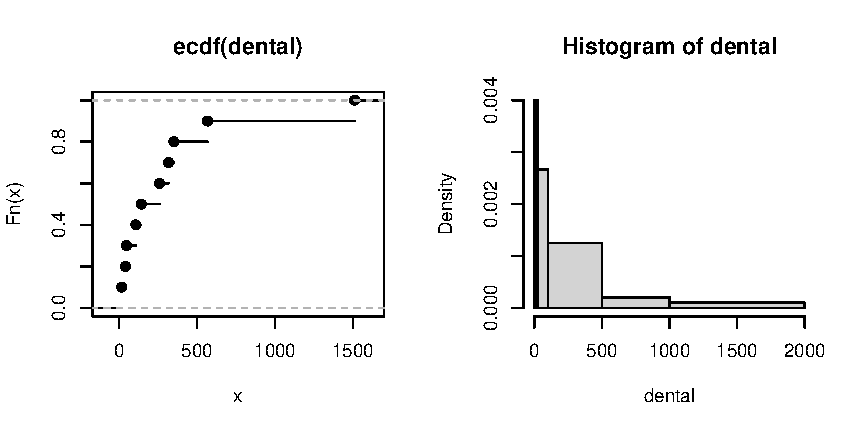
\includegraphics{cjs-rcs-figure}
%   \caption{\ifenglish A sample figure\else Exemple de figure\fi}
%   \label{fig:authguide:sample-figure}
% \end{figure}
%
% \ifenglish%
% If a figure requires an external file, you must provide it with your
% final version, usually in EPS, PDF or PNG format: see %
% \else%
% Si une figure requiert un fichier externe, vous devrez le fournir
% avec votre version finale, habituellement en format EPS, PDF ou PNG;
% consultez les %
% \fi
% \href{https://authorservices.wiley.com/author-resources/Journal-Authors/Prepare/manuscript-preparation-guidelines.html/figure-preparation.html}{%
%   \ifenglish Wiley's guidelines for the preparation of figures\relax
%   \else directives de Wiley pour la préparation des figures\fi}. %
%
% \ifenglish%
% Prepare tables as follows\relax%
% \else%
% Composez vos tableaux selon les règles suivantes\relax%
% \fi
% \footnote{%
%   \ifenglish%
%   These guidelines are adapted from the documentation of %
%   \else%
%   Ces règles sont adaptées de la documentation de %
%   \fi
%   \href{https://ctan.org/pkg/booktabs}{\pkg{booktabs}}.}: %
% \begin{itemize}
% \item %
%   \ifenglish%
%   no vertical lines; %
%   \else%
%   aucun filet vertical; %
%   \fi
% \item %
%   \ifenglish%
%   \cmdprint{\toprule} at the top; %
%   \else%
%   \cmdprint{\toprule} au début; %
%   \fi
% \item %
%   \ifenglish%
%   \cmdprint{\midrule} between the heading and body; %
%   \else%
%   \cmdprint{\midrule} entre l'entête et le corps; %
%   \fi
% \item%
%   \ifenglish%
%   \cmdprint{\bottomrule} at the bottom; %
%   \else%
%   \cmdprint{\bottomrule} au pied; %
%   \fi
% \item %
%   \ifenglish%
%   consistent number of decimal places thoughout the table; %
%   \else%
%   nombre de décimales uniforme; %
%   \fi
% \item %
%   \ifenglish%
%   leading digit in front of a decimal point ($0.1$, not $.1$).
%   \else%
%   marqueur des entiers devant les nombres décimaux ($0,1$ plutôt que
%   $,1$). %
%   \fi
% \end{itemize}
%
% \ifenglish%
% For table footnotes, use the package %
% \else%
% Pour les notes de contenu dans un tableau, utilisez %
% \fi%
% \href{https://ctan.org/pkg/threeparttable}{\pkg{threeparttable}}. %
% \ifenglish%
% However, place \cmdprint{\caption} \emph{outside} the environment
% \code{threeparttable} so that the caption can span the whole width
% of the page: %
% \else%
% Cependant, veillez à placer \cmdprint{\caption} à l'\emph{extérieur}
% de l'environnement \code{threeparttable} afin que la légende occupe
% toute la largeur de la page, le cas échéant: %
% \fi
% \iffalse
%<*example>
% \fi
  \def\CAPTION{\ifenglish caption\else légende\fi}
  \def\LABEL{\ifenglish label\else étiquette\fi}
  \def\TABLECONTENTS{\ifenglish table contents\else contenu du tableau\fi}
\begin{lstlisting}
\begin{table}
  \caption`\marg{\CAPTION}'
  \label`\marg{\LABEL}'
  \centering
  \begin{threeparttable}
    \begin{tabular}`\marg{cols}'
      `\meta{\TABLECONTENTS}'
    \end{tabular}
    \begin{tablenotes}
      `\meta{notes}'
    \end{tablenotes}
  \end{threeparttable}
\end{table}
\end{lstlisting}
% \iffalse
%</example>
% \fi
%
% \ifenglish%
% \section{Computer code and software}
% \else%
% \section{Code informatique et logiciels}
% \fi
% \label{sec:authguide:software}
%
% \ifenglish%
% Providing your computer code is a great way to increase the
% visibility of your work and its accessibility to end users of
% statistics. We strongly encourage that you share your code through a
% suitable repository, such as
% \else%
% Vous améliorerez la visibilité de vos travaux et leur dissémination
% parmi les utilisateurs de la statistique si vous fournissez votre
% code informatique. Nous vous encourageons fortement à partager
% celui-ci par le biais d'un dépôt ouvert, tel que %
% \fi
% \href{https://github.com/}{GitHub}
% \ifenglish or \else ou \fi %
% \href{https://gitlab.com/}{GitLab},
% \ifenglish%
% so that you can keep it up-to-date after the article has been
% published. Alternatively, you may provide your code in the
% Supplementary Material.
% \else%
% afin d'en permettre la mise à jour après la publication de
% l'article. Autrement, vous pouvez inclure le code dans le matériel
% additionnel. %
% \fi
%
% \ifenglish%
% The class does not offer any special features to typeset computer
% code. We recommend that you use specialized packages such
% as %
% \else%
% La classe ne propose aucune fonctionnalité particulière pour la
% présentation du code informatique. Nous vous recommandons d'avoir
% recours à des paquetages spécialisés comme %
% \fi
% \href{https://ctan.org/pkg/fancyvrb}{\pkg{fancyvrb}} %
% \ifenglish or \else ou \fi%
% \href{https://ctan.org/pkg/listings}{\pkg{listings}}. %
% \ifenglish%
% If you use {\Rlang} for your analysis, you could prepare the file
% using a literate programming system such as %
% \else%
% Si vous utilisez {\Rlang} pour effectuer votre analyse, vous pouvez
% rédiger l'article avec un système de programmation lettrée comme %
% \fi
% \href{https://en.wikipedia.org/wiki/Sweave}{Sweave} %
% \ifenglish or \else ou \fi%
% \href{https://en.wikipedia.org/wiki/Knitr}{knitr}.
%
% \ifenglish%
% That said, the class defines a few commands to ease and standardize
% the display of software names and code chunks. The command
% \cmd{\proglang} typesets the names of programming languages and
% software, and there are shortcuts for the most common cases; see
% \autoref{tab:authguide:proglang}. For example, refer to {\Rlang}
% using either \cmdprint{\proglang}\code{\{R\}} or
% \cmdprint{\Rlang}. The command \cmd{\pkg} typesets the names of
% software packages or modules. For example, refer to the {\Rlang}
% package \pkg{copula} using \cmdprint{\pkg}\code{\{copula\}}. %
% \else%
% Cela dit, la classe fournit quelques commandes pour faciliter et
% uniformiser la présentation des noms de logiciels et des extraits de
% code. La commande \cmd{\proglang} compose le nom des langages de
% programmation et des logiciels. Des raccourcis sont fournis pour les
% cas les plus usuels; voir le \autoref{tab:authguide:proglang}.
% Ainsi, pour mentionner {\Rlang}, utilisez
% \cmdprint{\proglang}\code{\{R\}} ou \cmdprint{\Rlang}. La commande
% \cmd{\pkg} compose le nom des paquetages ou modules logiciels. Par
% exemple, vous saisirez \cmdprint{\pkg}\code{\{copula\}} pour
% mentionner le paquetage {\Rlang} \pkg{copula}. %
% \fi
%
% \begin{table}
%   \ifenglish%
%   \caption{List of shortcuts for the names of programming languages
%   and software.}
%   \else%
%   \caption{Liste des raccourcis pour les noms de langages de
%   programmation et de logiciels}
%   \fi
%   \label{tab:authguide:proglang}
%   \centering
%   \begin{tabular}{ll}
%     \toprule
%     \ifenglish Software\else Logiciel\fi & \ifenglish Command\else Commande\fi \\
%     \midrule
%     \Rlang     & \cmd{\Rlang} \\
%     \SASlang   & \cmd{\SASlang} \\
%     \SPSSlang  & \cmd{\SPSSlang} \\
%     \Statalang & \cmd{\Statalang} \\
%     \Pylang    & \cmd{\Pylang} \\
%     \Julialang & \cmd{\Julialang} \\
%     \Clang     & \cmd{\Clang} \\
%     \Cpplang   & \cmd{\Cpplang} \\
%     \bottomrule
%   \end{tabular}
% \end{table}
%
% \ifenglish%
% For small chunks of code, such as the names of exploratory variables
% in a regression model, \cmd{\code} may be useful: it allows you to
% use the characters \code{_}, \code{~} and \code{$} directly. For
% example, you may write \cmdprint{\code}\code{\{patient_age\}} to get
% \code{patient_age}. %
% \else%
% La commande \cmd{\code} est utile pour composer de courts extraits
% de code, comme les noms des variables d'un modèle de régression. La
% commande permet d'utiliser directement les caractères «\code{_}»,
% «\code{~}» et «\code{$}». Par exemple, vous pouvez entrer
% \cmdprint{\code}\code{\{patient_age\}} pour obtenir
% \code{patient_age}. %
% \fi
%
% \ifenglish%
% Remember to report the software packages you used and their
% version numbers; see the following section. %
% \else%
% Vous devez toujours mentionner les logiciels utilisés, ainsi que
% leur version. La section suivante fournit plus de détails à ce
% sujet.
% \fi
%
% \ifenglish%
% \section{Citations and references}
% \else%
% \section{Citations et références}
% \fi
% \label{sec:authguide:references}
%
% \ifenglish%
% For citations and references, use {\BibTeX}. Recall that %
% \else%
% Utilisez {\BibTeX} pour les citations et les références. Tel que
% mentionné précédemment, le paquetage %
% \fi%
% \href{https://ctan.org/pkg/natbib}{\pkg{natbib}} %
% \ifenglish%
% is loaded automatically. Please use the \cmd{\citet} and
% \cmd{\citep} commands of \pkg{natbib}.
% \else%
% est chargé automatiquement par la classe. Assurez-vous
% d'utiliser ses commandes \cmd{\citet} et \cmd{\citep}. %
% \fi
%
% \ifenglish%
% The class also uses its own bibliography styles. These styles
% support the standard {\BibTeX} entry types %
% \else%
% La classe a également recours à ses propres styles de bibliographie.
% Ceux-ci prennent en charge les types d'entrées standards de
% {\BibTeX} %
% \fi
% (\code{article}, \code{book}, \code{proceedings}, etc.) %
% \ifenglish%
% and the standard fields %
% \else%
% et les champs standards %
% \fi%
% (\code{author}, \code{title}, \code{journal}, etc.). %
% \ifenglish%
% Furthermore, the styles support %
% \else%
% De plus, ils ajoutent les champs %
% \fi%
% \code{doi}, \code{isbn}, \code{url} \ifenglish and \else et \fi
% \code{language}.
% \ifenglish%
% These are explained in the examples below. %
% \else%
% Les exemples ci-dessous illustrent chacun de ces champs. %
% \fi%
%
% \begin{itemize}
% \item %
%   \ifenglish%
%   Articles with one author: \citet{Genest:1999}. To include a
%   DOI, use the field \code{doi} with a value in the format
%   \meta{prefix}\code{/}\meta{suffix} (for example,
%   \code{10.2307/3315650}). A hyperlink to the resource is then
%   created automatically. Note that journal names should not be
%   abbreviated. %
%   \else%
%   Articles avec un auteur unique: \citet{Genest:1999}. Pour ajouter
%   un identificateur DOI, utilisez le champ \code{doi} avec une valeur
%   de la forme \meta{préfixe}\code{/}\meta{suffixe} (par exemple:
%   \code{10.2307/3315650}). Un hyperlien vers la ressource est créé
%   automatiquement. Inscrivez les noms des journaux au long. %
%   \fi
% \item %
%   \ifenglish%
%   Articles with two authors: \citet{Qin/Lawless:1995}. Articles
%   with three or more authors: \citet{Davison/Fraser/Reid:2006} or
%   \citet{Granville:2023}. For articles with more than ten authors
%   \citep[such as][]{Teufel:2016}, give the first seven names
%   followed by ``and others''. {\BibTeX} will replace this by
%   ``et~al.''
%   \else%
%   Articles avec deux auteurs: \citet{Qin/Lawless:1995}. Articles
%   avec trois auteurs ou plus: \citet{Davison/Fraser/Reid:2006} ou
%   encore \citet{Granville:2023}. Pour les articles comptant plus de
%   dix auteurs \citep[par exemple:][]{Teufel:2016}, inscrivez les
%   noms des sept premiers auteurs, suivis de \emph{and others}.
%   {\BibTeX} inscrira automatiquement «et collab.» dans la notice.
%   \fi
% \item %
%   \ifenglish%
%   Use the field \code{language} for foreign-language articles, as in
%   \citet{Hoeffding:1940} (German) or
%   \citet{Ghoudi/Khoudraji/Rivest:1998} (French). Including this
%   information in the {\BibTeX} entry ensures that the title words
%   are hyphenated according to the rules of the corresponding
%   language. %
%   \else%
%   Le champ \code{language} permet d'indiquer la langue d'une notice
%   lorsqu'elle diffère de celle de l'article. C'est important pour la
%   coupure de mots dans les titres. Par exemple, pour le présent
%   document en français, la plupart des entrées de la bibliographie
%   déclarent l'anglais comme langue, alors que \citet{Hoeffding:1940}
%   déclare l'allemand. En revanche,
%   \citet{Ghoudi/Khoudraji/Rivest:1998} déclare le français pour la
%   version anglaise du document. %
%   \fi
% \item %
%   \ifenglish%
%   Books and other formats use the same author rules as articles.
%   An example of a book with two authors is
%   \citet{Kalbfleisch/Prentice:2002}. You may use \code{isbn} to include
%   the book's ISBN. Include the relevant page, section, or chapter
%   whenever possible in \cmd{\citet} and \cmd{\citep}. For example,
%   partial likelihood estimation in the Cox regression model may be
%   found in %
%   \else%
%   Les règles pour les auteurs de livres et autres types d'entrées
%   sont les mêmes que pour les articles.
%   \citet{Kalbfleisch/Prentice:2002} est un exemple de livre comptant
%   deux auteurs. Utilisez le champ \code{isbn} pour préciser le
%   numéro ISBN de l'ouvrage. Quand vous citez un livre, précisez
%   autant que faire se peut la page, la section ou le chapitre dans
%   les commandes \cmd{\citet} et \cmd{\citep}. Par exemple,
%   l'estimation par vraisemblance partielle dans le modèle de
%   régression de Cox est traitée dans %
%   \fi
%   \citet[\ifenglish Section\else section\fi~4.2]{Kalbfleisch/Prentice:2002}; %
%   \ifenglish see also \else voir aussi \fi %
%   \citet[\ifenglish Chapter\else chapitre\fi~6]{Kalbfleisch/Prentice:2002}.
% \item %
%   \ifenglish%
%   For references to articles in an edited book, include the page
%   numbers of the article, as well as the names of the book's
%   editors, such as \citet{Roberts:2009}. Again, we encourage you to
%   include the DOI. %
%   \else%
%   Pour la notice d'une partie d'un ouvrage collectif, précisez les
%   pages de la partie citée ainsi que les noms des éditeurs, tel que
%   dans \citet{Roberts:2009}. Ici aussi, nous vous invitons à inclure
%   un identificateur DOI. %
%   \fi
% \item %
%   \ifenglish%
%   You may need to cite a PhD thesis such as \citet{Syed:2022} or a
%   technical report such as \citet{Haas:2001} or an unpublished
%   manuscript posted on arXiv such as \citet{Tang/Kong/Wang:2023}.
%   If you have a DOI or URL, include it in the entry using \code{doi}
%   or \code{url}. If both are present in the database, the DOI
%   takes precedence.
%   \else%
%   Vous pouvez citer une thèse de doctorat \citep{Syed:2022}, un
%   rapport technique \citep{Haas:2001} ou une publication
%   préliminaire dans arXiv \citep{Tang/Kong/Wang:2023}. Saisissez les
%   identificateur DOI et les adresses URL avec les champs \code{doi}
%   et \code{url}. Lorsque les deux sont présents dans la base de
%   données, l'identificateur DOI a priorité. %
%   \fi
% \item %
%   \ifenglish%
%   Cite the software you used in your statistical analysis,
%   especially Free Software. To cite {\Rlang}, use the {\BibTeX}
%   entry provided by the command %
%   \else%
%   Citez les logiciels utilisés pour vos analyses statistiques, tout
%   particulièrement les logiciels libres. Pour citer {\Rlang},
%   utilisez l'entrée {\BibTeX} produite par la commande %
%   \fi
% \iffalse
%<*example>
% \fi
\begin{lstlisting}
> citation()
\end{lstlisting}
% \iffalse
%</example>
% \fi
%   \ifenglish%
%   Don't forget to include the version of {\Rlang}, as in:
%   ``Computations in this article were performed using {\Rlang}
%   \citep[v4.5.0]{Rlang}''. You can get this via:
%   \else%
%   N'oubliez pas d'inclure aussi la version de {\Rlang} dans une
%   mention de la forme «Les calculs de cet article ont été effectués
%   avec {\Rlang} \citep[v4.5.0]{Rlang}». L'expression {\Rlang}
%   suivante fournit la version du logiciel: %
%   \fi
% \iffalse
%<*example>
% \fi
\begin{lstlisting}
> R.version.string
\end{lstlisting}
% \iffalse
%</example>
% \fi
%   \ifenglish%
%   To cite an {\Rlang} package, use the command \code{citation} with
%   the name of the package in argument, e.g.\ %
%   \else%
%   Pour citer un paquetage {\Rlang}, utilisez aussi la commande
%   \code{citation}, mais en ajoutant le nom du paquetage en
%   argument: %
%   \fi
% \iffalse
%<*example>
% \fi
\begin{lstlisting}
> citation("copula")
\end{lstlisting}
% \iffalse
%</example>
% \fi
%   \ifenglish%
%   This specific example asks you to cite three articles
%   \citep{Yan:2007,Kojadinovic/Yan:2010,Hofert/Maechler:2011} as well
%   as the software itself \citep{Rcopula:2024}.
%   \else%
%   Dans cet exemple en particulier, on demande de citer trois
%   articles
%   \citep{Yan:2007,Kojadinovic/Yan:2010,Hofert/Maechler:2011} en plus
%   du logiciel lui-même \citep{Rcopula:2024}. %
%   \fi
% \item %
%   \ifenglish%
%   To cite data, please review %
%   \else%
%   Si vous devez citer des données, consultez la %
%   \fi
%   \href{https://authorservices.wiley.com/author-resources/Journal-Authors/open-access/data-sharing-citation/data-citation-policy.html}{%
%     \ifenglish Wiley's data citation policy\relax
%     \else politique de citation des données de Wiley\fi}. %
%   \ifenglish%
%   An example of a data citation is \citet{StatCan:2023}.
%   \else%
%   Un exemple de citation de données est \citet{StatCan:2023-fr}.
%   \fi
% \item %
%   \ifenglish%
%   You can also cite a webpage, for example \citet{Wolfram:2010}.
%   Include the date of access using the \code{note} field. %
%   \else%
%   Vous pouvez citer une page web, par exemple \citet{Wolfram:2010}.
%   Précisez la date de consultation de la page dans le champ
%   \code{note}. %
%   \fi
% \end{itemize}
%
% \appendix
%
% \ifenglish%
% \section{Proofs}
% \else%
% \section{Démonstrations}
% \fi
% \label{sec:authguide:proofs}
%
% \ifenglish%
% Appendices usually present original proofs or longer mathematical
% derivations; don't forget to cite them in the main article. You
% may structure each appendix into multiple sections and
% subsections. %
% \else%
% Les annexes sont habituellement réservées aux démonstrations ou
% longs développements mathématiques. Vous devez les citer dans le
% corps de l'article. Vous pouvez diviser les annexes en sections et
% sous-sections. %
% \fi
%
% \ifenglish%
% \section{Supplementary material}
% \else%
% \section{Matériel additionnel}
% \fi
% \label{sec:authguide:supplement}
%
% \ifenglish%
% To make your article accessible to a wide readership and to control
% its length, consider providing online supplementary material, citing
% it in the main article. It may contain additional simulation
% results, lengthy tables or figures, auxiliary results, proofs that
% are direct adaptations of calculations already published elsewhere,
% details about the code and software implementation, and so on. That
% said, we encourage you to place original mathematical proofs in an
% appendix and to present the ideas behind these proofs in the main
% text. %
% \else%
% Le matériel additionnel rendu disponible en ligne permet d'élargir
% le lectorat de votre article tout en limitant sa longueur. Vous
% devez citer le matériel additionnel dans l'article. Celui-ci peut
% contenir, entre autres, des résultats de simulation additionnels, de
% longs tableaux ou de grandes figures, des résultats auxiliaires, des
% démonstrations qui sont des applications directes de résultats déjà
% publiés ailleurs, des détails à propos de la mise en œuvre
% informatique. Attention, toutefois: les démonstrations originales
% sont mieux à leur place dans une annexe. Présentez simplement les
% idées fortes derrière celles-ci dans le corps du texte. %
% \fi
%
% \ifenglish%
% To prepare the supplementary material, use the option
% \code{supplement}: %
% \else%
% Pour préparer le matériel additionnel, utilisez l'option
% \code{supplement} de la classe: %
% \fi
% \iffalse
%<*example>
% \fi
\begin{lstlisting}
\documentclass[`\LANGOPT',supplement]{cjs-rcs-article}
\end{lstlisting}
% \iffalse
%</example>
% \fi
% \ifenglish%
% or, to make the supplement suitable for review, %
% \else%
% ou, pour anonymiser le matériel additionnel en vue de l'évaluation
% par les pairs,
% \fi
% \iffalse
%<*example>
% \fi
\begin{lstlisting}
\documentclass[`\LANGOPT',supplement,review]{cjs-rcs-article}
\end{lstlisting}
% \iffalse
%</example>
% \fi
% \ifenglish%
% Your supplementary material is published as supplied, and a proof is
% not made available, so be sure to double-check the file and to
% provide the material in its final format. %
% \else%
% Nous publions votre matériel additionnel tel quel; aucune épreuve ne
% vous sera fournie. Assurez-vous donc de la conformité de votre
% fichier. %
% \fi
%
% \vspace*{10pt}
% \hfill
% \ifenglish%
%   \emph{Have fun writing!}
% \else%
%   \emph{Bonne rédaction!}
% \fi%
%
% \begin{thebibliography}{23}
% \providecommand{\natexlab}[1]{#1}
% \providecommand{\url}[1]{\texttt{#1}}
% \providecommand{\urlprefix}{}
% \providecommand{\doiprefix}{doi: }
% \expandafter\ifx\csname href\endcsname\relax
%   \providecommand{\urldoi}[1]{#1}\else
%   \providecommand{\urldoi}[1]{\href{https://doi.org/#1}{#1}}\fi
% \providecommand{\selectlanguage}[1]{\relax}
% 
% \bibitem[{Davison et~al.(2006)Davison, Fraser, and
%   Reid}]{Davison/Fraser/Reid:2006}
% Davison, A.~C., Fraser, D. A.~S., and Reid, N. (2006).
% \newblock {\selectlanguage{english}Improved likelihood inference for discrete
%   data}.
% \newblock \emph{Journal of the Royal Statistical Society Series B: Statistical
%   Methodology}, 68(3):495--508.
% \newblock \doiprefix\urldoi{10.1111/j.1467-9868.2006.00548.x}.
% 
% \bibitem[{Downes and Beeton(2017)}]{Downes:short-math-guide:2017}
% Downes, M. and Beeton, B. (2017).
% \newblock {\selectlanguage{english}\emph{Short Math Guide for {\LaTeX}}}.
% \newblock American Mathematical Society.
% \newblock \urlprefix\url{https://ctan.org/pkg/short-math-guide}.
% 
% \bibitem[{Genest(1999)}]{Genest:1999}
% Genest, C. (1999).
% \newblock {\selectlanguage{english}Probability and statistics: A tale of two
%   worlds?}
% \newblock \emph{The Canadian Journal of Statistics}, 27(2):421--444.
% \newblock \doiprefix\urldoi{10.2307/3315650}.
% 
% \bibitem[{Ghoudi et~al.(1998)Ghoudi, Khoudraji, and
%   Rivest}]{Ghoudi/Khoudraji/Rivest:1998}
% Ghoudi, K., Khoudraji, A., and Rivest, L.-P. (1998).
% \newblock {\selectlanguage{french}Propri\'et\'es statistiques des copules de
%   valeurs extr\^emes bidimensionnelles}.
% \newblock \emph{The Canadian Journal of Statistics}, 26:187--197.
% \newblock \doiprefix\urldoi{10.2307/3315683}.
% 
% \bibitem[{Granville et~al.(2023)Granville, Woolford, Dean, Boychuk, and
%   McFayden}]{Granville:2023}
% Granville, K., Woolford, D.~G., Dean, C.~B., Boychuk, D., and McFayden, C.~B.
%   (2023).
% \newblock {\selectlanguage{english}On the selection of an interpolation method
%   with an application to the {F}ire {W}eather {I}ndex in {O}ntario, {C}anada}.
% \newblock \emph{Environmetrics}, 34(2):e2758.
% \newblock \doiprefix\urldoi{10.1002/env.2758}.
% 
% \bibitem[{Haas(2001)}]{Haas:2001}
% Haas, M. (2001).
% \newblock {\selectlanguage{english}\emph{New Methods in Backtesting}}.
% \newblock Tech. rep., Financial Engineering Research Center, Bonn, Germany.
% \newblock \urlprefix\url{https://www.yumpu.com/s/L9EC3aHSgRvWa763}.
% 
% \bibitem[{Higham(2020)}]{Higham:2020}
% Higham, N.~J. (2020).
% \newblock {\selectlanguage{english}\emph{Handbook of Writing for the
%   Mathematical Sciences}}.
% \newblock 3rd ed. SIAM, Philadelphia.
% \newblock ISBN 978-1-61197-609-0.
% \newblock \doiprefix\urldoi{10.1137/1.9781611976106}.
% 
% \bibitem[{Hoeffding(1940)}]{Hoeffding:1940}
% Hoeffding, W. (1940).
% \newblock {\selectlanguage{german}Ma{\ss}stabinvariante {K}orrelationstheorie
%   f\"ur diskontinuierliche {V}erteilungen}.
% \newblock \emph{Archiv f\"ur mathematische Wirtschafts- und Sozialforschung},
%   7:4--70.
% 
% \bibitem[{Hofert et~al.(2023)Hofert, Kojadinovic, Maechler, and
%   Yan}]{Rcopula:2024}
% Hofert, M., Kojadinovic, I., Maechler, M., and Yan, J. (2023).
% \newblock {\selectlanguage{english}\emph{copula: Multivariate Dependence with
%   Copulas}}.
% \newblock \urlprefix\url{https://cran.r-project.org/package=copula}.
% \newblock R package version 1.1-4.
% 
% \bibitem[{Hofert and M\"achler(2011)}]{Hofert/Maechler:2011}
% Hofert, M. and M\"achler, M. (2011).
% \newblock {\selectlanguage{english}Nested {A}rchimedean copulas meet {R}: The
%   {nacopula} package}.
% \newblock \emph{Journal of Statistical Software}, 39(9):1--20.
% \newblock \doiprefix\urldoi{10.18637/jss.v039.i09}.
% 
% \bibitem[{Kalbfleisch and Prentice(2002)}]{Kalbfleisch/Prentice:2002}
% Kalbfleisch, J.~D. and Prentice, R.~L. (2002).
% \newblock {\selectlanguage{english}\emph{The Statistical Analysis of Failure
%   Time Data}}.
% \newblock 2nd ed. Wiley Series in Probability and Statistics,
%   Wiley-Interscience [John Wiley \& Sons], Hoboken, NJ.
% \newblock ISBN 9780471363576.
% \newblock \doiprefix\urldoi{10.1002/9781118032985}.
% 
% \bibitem[{Kojadinovic and Yan(2010)}]{Kojadinovic/Yan:2010}
% Kojadinovic, I. and Yan, J. (2010).
% \newblock {\selectlanguage{english}Modeling multivariate distributions with
%   continuous margins using the {copula} {R} package}.
% \newblock \emph{Journal of Statistical Software}, 34(9):1--20.
% \newblock \doiprefix\urldoi{10.18637/jss.v034.i09}.
% 
% \bibitem[{Mermin(1989)}]{Mermin:1989}
% Mermin, N.~D. (1989).
% \newblock {\selectlanguage{english}What's wrong with these equations?}
% \newblock \emph{Physics Today}, 42(10):9--11.
% \newblock \doiprefix\urldoi{10.1063/1.2811173}.
% 
% \bibitem[{Oetiker et~al.(2021)Oetiker, Partl, Hyna, and
%   Schlegl}]{Oetiker:lshort-english:2021}
% Oetiker, T., Partl, H., Hyna, I., and Schlegl, E. (2021).
% \newblock {\selectlanguage{english}\emph{The Not So Short Introduction to
%   {\LaTeXe}}}.
% \newblock \urlprefix\url{https://ctan.org/pkg/lshort-english}.
% \newblock Version 6.4.
% 
% \bibitem[{Qin and Lawless(1995)}]{Qin/Lawless:1995}
% Qin, J. and Lawless, J. (1995).
% \newblock {\selectlanguage{english}Estimating equations, empirical likelihood
%   and constraints on parameters}.
% \newblock \emph{The Canadian Journal of Statistics}, 23(2):145--159.
% \newblock \doiprefix\urldoi{10.2307/3315441}.
% 
% \bibitem[{{R Core Team}(2024)}]{Rlang}
% {R Core Team} (2024).
% \newblock {\selectlanguage{english}\emph{R: A Language and Environment for
%   Statistical Computing}}.
% \newblock R Foundation for Statistical Computing, Vienna, Austria.
% \newblock \urlprefix\url{https://www.r-project.org/}.
% 
% \bibitem[{Roberts et~al.(2009)Roberts, Ren, and Rao}]{Roberts:2009}
% Roberts, G., Ren, Q., and Rao, J. N.~K. (2009).
% \newblock {\selectlanguage{english}Using marginal mean models for data from
%   longitudinal surveys with a complex design: Some advances in methods}.
% \newblock In R.~Lynn, editor, \emph{Methodology of Longitudinal Surveys}, pages
%   351--366. John Wiley \& Sons, New York.
% \newblock ISBN 9780470018712.
% \newblock \doiprefix\urldoi{10.1002/9780470743874}.
% 
% \bibitem[{{Statistics Canada}(2023)}]{StatCan:2023}
% {Statistics Canada} (2023).
% \newblock {\selectlanguage{english}Table 13-10-0096-01 {H}ealth
%   characteristics, annual estimates, inactive}.
% \newblock \doiprefix\urldoi{10.25318/1310009601-eng}.
% 
% \bibitem[{Syed(2022)}]{Syed:2022}
% Syed, S. (2022).
% \newblock {\selectlanguage{english}\emph{Non-reversible parallel tempering on
%   optimized paths}}.
% \newblock Ph.D. thesis, University of British Columbia, Vancouver (BC), Canada.
% \newblock \doiprefix\urldoi{10.14288/1.0413120}.
% 
% \bibitem[{Tang et~al.(2023)Tang, Kong, and Wang}]{Tang/Kong/Wang:2023}
% Tang, D., Kong, D., and Wang, L. (2023).
% \newblock {\selectlanguage{english}The synthetic instrument: From sparse
%   association to sparse causation}.
% \newblock arXiv.
% \newblock \doiprefix\urldoi{10.48550/arXiv.2304.01098}.
% 
% \bibitem[{Teufel et~al.(2016)Teufel, Diro, Whan, Milrad, Jeong, Ganji, Huziy
%   et~al.}]{Teufel:2016}
% Teufel, B., Diro, G.~T., Whan, K., Milrad, S.~M., Jeong, D.~I., Ganji, A.,
%   Huziy, O. et~al. (2016).
% \newblock {\selectlanguage{english}Investigation of the 2013 {A}lberta flood
%   from a weather/climate perspective}.
% \newblock \emph{Climate Dynamics}, 48(9):2881--2899.
% \newblock \doiprefix\urldoi{10.1007/s00382-016-3239-8}.
% 
% \bibitem[{{W}olfram {R}esearch(2010)}]{Wolfram:2010}
% {W}olfram {R}esearch (2010).
% \newblock {\selectlanguage{english}Pearson distribution}.
% \newblock
%   \urlprefix\url{https://reference.wolfram.com/language/ref/PearsonDistribution.html}.
% \newblock Accessed October 12, 2022.
% 
% \bibitem[{Yan(2007)}]{Yan:2007}
% Yan, J. (2007).
% \newblock {\selectlanguage{english}Enjoy the joy of copulas: With a package
%   copula}.
% \newblock \emph{Journal of Statistical Software}, 21(4):1--21.
% \newblock \doiprefix\urldoi{10.18637/jss.v021.i04}.
% 
% \end{thebibliography}
%
% \ifenglish%
%   \PrintChanges
% \else%
%   \section*{Historique des versions}
%   \label{sec:authguide:implementation}
%   Consultez la version anglaise de ce document pour l'historique des
%   versions. %
% \fi

%</fr-doc>
% \fi
% \GetFileInfo{cjs-rcs-authguide.dtx}
% \expandafter\parsedate\filedate\relax
%
% \changes{2.0}{2026-03-05}{Adapt the guidelines to the single-blind
% review process.}
% \changes{1.3}{2025-08-29}{Improve the French version in a few
% places.}
% \changes{1.2c}{2025-08-11}{Add guidelines on the length and contents
% of the abstracts.}
% \changes{1.2b}{2025-07-25}{Fix the link to instructions on updating
% a {\TeX} distribution.}
% \changes{1.2b}{2025-07-25}{Improve the text of the French version in
% a few places and fix typos.}
% \changes{1.2b}{2025-07-25}{Use the French variant of the reference
% Statistics Canada (2023) in the French version.}
% \changes{1.2a}{2025-07-24}{Fix the typesetting of a few entries in
% the list of references.}
% \changes{1.2a}{2025-07-24}{Provide more specific URLs for Oetiker et
% al. (2021) and Oetiker et collab. (2011).}
% \changes{1.2}{2025-07-10}{Initial version in the distribution.}
%
% \ifenglish%
% \makeatletter
% \title[Author guidelines for \CJS@journalname@en]{%
% Author guidelines \\ for \TheCJS}
% \makeatother
% \author{\SSCen}
% \affil{Guidelines developed by Julie Falkner, Vincent Goulet,
% Johanna Nešlehová}
% \runningauthor{Statistical Society of Canada}
% \else%
% \makeatletter
% \title[Directives pour les auteurs de \CJS@journalname@fr]{%
%   Directives pour les auteurs \\ de \LaRevue}
% \makeatother
% \author{\SSCfr}
% \affil{Directives rédigées par Julie Falkner, Vincent Goulet,
% Johanna Nešlehová}
% \runningauthor{Société canadienne de statistique}
% \fi
%
% \begin{englishabstract}
%   This guide provides the stylistic and presentation guidelines
%   for authors submitting an article to {\TheCJS}. Although the
%   guidelines apply broadly, the document assumes that the
%   manuscript is prepared using {\LaTeX} and the class
%   {\CJSclass}. This guide is also available in%
%   \ifenglish French\else English\fi.
% \end{englishabstract}
% \begin{frenchabstract}
%   Ce guide fournit les directives en matière de style et de
%   présentation pour les auteurs qui soumettent un article dans
%   {\LaRevue}. Les directives s'appliquent de manière générale, mais
%   le document se concentre sur la préparation d'un manuscript avec
%   {\LaTeX} et la classe {\CJSclass}. Ce guide est aussi disponible
%   en \ifenglish français\else anglais\fi.
% \end{frenchabstract}
%
% ^^A abusing the 'classification' environment. The final period is
% ^^A added by the environment.
% \begin{classification}[Version]
% \item[] %
%   \ifenglish%
%   These guidelines accompany the class {\CJSclass}~{\fileversion},
%   dated {\filedate} %
%   \else%
%   Ces directives accompagnent la classe {\CJSclass}~{\fileversion},
%   datée du {\filedate} %
%   \fi
% \end{classification}
%
% \licence{{\ccbysa*} 2025--{\year}, {\SSCen}~{\textbar}~{\SSCfr}}
%
% \makeCJStitle
%
% \section{Introduction}
% \label{sec:authguide:introduction}
%
% \ifenglish%
% This document provides guidelines for authors of {\TheCJS}. Please
% read them carefully: manuscripts that are scientifically acceptable
% but don't follow these stylistic guidelines will need additional
% work by the editors and copy-editors, delaying publication. %
% \else%
% Le présent document fournit les directives aux auteurs de
% {\LaRevue}. Lisez-le avec attention, car un manuscript
% scientifiquement acceptable verra sa publication retardée par le
% travail d'édition additionnel requis s'il ne respecte pas les
% directives en matière de style. %
% \fi
%
% \ifenglish%
% Manuscripts may be submitted in either English or French. We accept
% submissions in Microsoft~Word, but authors are encouraged to use
% {\LaTeX} and the class {\CJSclass}, described in this guide. You'll
% find documentation and additional information at the %
% \href{\siteurl}{project website}. %
% \else%
% Vous pouvez soumettre votre manuscript en français comme en anglais.
% Bien que nous acceptions le format Microsoft Word, nous recommandons
% d'utiliser {\LaTeX} et la classe {\CJSclass}. C'est d'ailleurs le
% mode de préparation décrit dans le présent guide. Vous trouverez de
% la documentation et des informations additionnelles dans le %
% \href{\siteurl/fr}{site web du projet}. %
% \fi%
%
% \ifenglish%
% Using {\CJSclass} requires an up-to-date {\TeX} distribution, so
% start by %
% \else%
% La classe {\CJSclass} requiert une distribution {\TeX} à jour, alors
% assurez-vous avant toute chose d'en %
% \fi
% \href{https://tex.stackexchange.com/q/55437}{\ifenglish doing this
% update\else effectuer la mise à jour\fi}. %
% \ifenglish%
% Since the class is part of the standard {\TeX} distributions via the
% package {\CJSpkg}, it will also get installed or updated. %
% \else
% Puisque la classe fait partie des distributions {\TeX} standards via
% le paquetage {\CJSpkg}, elle sera de ce fait installée ou mise à
% jour. %
% \fi
%
% \tipbox{%
%   \ifenglish%
%   If you get error messages about missing or outdated packages when
%   using {\CJSclass}, the solution is to update your {\TeX}
%   distribution. %
%   \else%
%   Si vous obtenez des messages d'erreur au sujet de paquetages
%   manquants ou obsolètes en utilisant {\CJSclass}, c'est que vous
%   devez mettre à jour de votre distribution {\TeX}. %
%   \fi}
%
% \ifenglish%
% \section{Preparing your article}
% \else%
% \section{Mise en place de l'article}
% \fi
% \label{sec:authguide:preparing}
%
% \ifenglish%
% Don't start from scratch. The class ships with templates for
% articles in English and French. If you're using the version included
% with your {\TeX} distribution, the templates are located with the
% documentation of the class. You may also obtain them from %
% \else%
% Ne partez pas de zéro. La classe est livrée avec des gabarits pour
% des articles en français et en anglais. Si vous utilisez la version
% fournie avec votre distribution {\TeX}, les gabarits sont classés
% avec la documentation de la classe. Vous pouvez aussi les récupérer
% depuis %
% \fi%
% \href{https://ctan.org/pkg/\CJSname}{CTAN}. %
% \ifenglish%
% Copy the template to your working directory and follow the
% instructions and examples therein. You may also compile the template
% as is, obtaining a complete sample article. %
% \else%
% Copiez le gabarit dans votre dossier de travail et suivez les
% directives et les exemples qui s'y trouvent. Vous pouvez compiler le
% gabarit tel quel pour produire un exemple d'article complet. %
% \fi
%
% \changes{1.3}{2025-08-27}{Instruct, in the introduction of
% \emph{Preparing your article}, to type non-ASCII characters directly
% rather than by using {\TeX} commands.}
% \ifenglish%
% If you need non-ASCII characters (such as accented letters) in your
% manuscript, type them directly instead of using {\TeX} commands
% (e.g.~\code{é} and \code{ü} instead of \code{{\bs}'e} and
% \code{{\bs}"u}), and save your file using %
% \else%
% Si vous avez recours à des caractères non-ASCII (comme des lettres
% accentuées), entrez directement ceux-ci au clavier, sans passer par
% les commandes {\TeX} (par exemple: «\code{é}» et «\code{ü}» plutôt
% que «\code{{\bs}'e}» et «\code{{\bs}"u}»). Enregistrez le fichier
% dans le codage de caractères %
% \fi%
% \href{https://fr.wikipedia.org/wiki/UTF-8}{UTF-8} %
% \ifenglish%
% character encoding. We recommend that you compile with {\LuaLaTeX},
% which allows for modern multilingual typesetting. Various packages
% are available with {\CJSclass} and there's no need to load them
% again: these include %
% \else%
% et compilez avec {\LuaLaTeX} pour tirer pleinement profit des
% caractéristiques de {\CJSclass}. Plusieurs paquetages étant chargés
% par la classe, vous n'avez pas besoin de les charger de nouveau.
% Parmi ceux-ci, mentionnons:%
% \fi
% \pkg{amsmath}, %
% \pkg{amsthm}, %
% \pkg{babel}, %
% \pkg{enumitem}, %
% \pkg{fontawesome5}, %
% \pkg{graphicx}, %
% \pkg{natbib}, %
% \pkg{numprint}, %
% \pkg{relsize}, %
% \pkg{url}\ifenglish, and \else\ et \fi %
% \pkg{xcolor}. %
%
% \ifenglish%
% \subsection{Class declaration}
% \else%
% \subsection{Déclaration de la classe}
% \fi
% \label{sec:authguide:preparing:documentclass}
%
% \ifenglish%
% The class requires the options \code{english} and \code{french}. The
% order is important: the \emph{second} one is the main language.
% Therefore, for an article in English use: %
% \else%
% Vous devez charger la classe avec les options \code{english} et
% \code{french}. Leur ordre est important: la \emph{seconde} est la
% langue principale de l'article. Par conséquent, pour un article en
% français, chargez la classe avec: %
% \fi
% \iffalse
%<*example>
% \fi
\def\LANGOPT{\ifenglish french,english\else english,french\fi}
\begin{lstlisting}
\documentclass[`\LANGOPT']{cjs-rcs-article}
\end{lstlisting}
% \iffalse
%</example>
% \fi%
%
% \ifenglish%
% \subsection{Title page}
% \else%
% \subsection{Page de titre}
% \fi
% \label{sec:authguide:preparing:titling}
%
% \ifenglish%
% Your preamble will contain the following declarations: %
% \else%
% Le préambule de votre manuscript doit contenir les déclarations
% suivantes pour produire les informations de la page de titre. %
% \fi
%
% \begin{itemize}
% \item %
%   \ifenglish%
%   \cmd{\title}: title of the article. See
%   \autoref{sec:authguide:typesetting:titles} for more on titles. Break a
%   long title covering more than one line using using \code{\bs\bs} or
%   \cmdprint{\newline}. If the title doesn't fit in the running head,
%   supply a short title as an optional argument (between square
%   brackets \texttt{[~]}): %
%   \else%
%   \cmd{\title}: titre de l'article; voir la
%   \autoref{sec:authguide:typesetting:titles} pour des détails
%   additionnels sur la composition du titre. Coupez manuellement un
%   titre qui nécessite plus d'une ligne avec \code{\bs\bs} ou
%   \cmdprint{\newline}. Si le titre est trop long pour l'entête,
%   fournissez une version courte en argument optionnel (entre les
%   crochets \texttt{[~]}): %
%   \fi%
%   \iffalse
%<*example>
%   \fi
\def\OPT{\ifenglish Short title\else Titre court\fi}
\def\ARG{\ifenglish Full title\else Titre complet\fi}
\begin{lstlisting}
\title`\oarg{\OPT}\marg{\ARG}'
\end{lstlisting}
%   \iffalse
%</example>
%   \fi
% \item %
%   \ifenglish%
%   \cmd{\author} and \cmd{\affil}: author name, ORCID~iD, email and
%   affiliation (give the country name in the language of the
%   article). The corresponding author is specified by
%   \code{corresponding} and surnames via \cmd{\surname}: %
%   \else%
%   \cmd{\author} et \cmd{\affil}: noms, identifiants ORCID, adresses
%   courriel et affiliations des auteurs (indiquez le nom du pays dans
%   la langue de l'article). Indiquez l'auteur correspondant avec
%   \code{corresponding} et entrez les noms de famille avec
%   \cmd{\surname}: %
%   \fi%
%   \iffalse
%<*example>
%   \fi
\def\EMAIL{\ifenglish email\else courriel\fi}
\def\FORENAME{\ifenglish Forename\else Prénom\fi}
\def\SURNAME{\ifenglish Surname\else Nom\fi}
\def\AFFIL{\ifenglish Department, University, City, Country\else%
  Département, Université, Ville, Pays\fi}
\begin{lstlisting}
\author[orcid=`\meta{id}', email=`\meta{\EMAIL}', corresponding]
       {`\meta{\FORENAME}' \surname`\marg{\SURNAME}'}
\affil`\marg{\AFFIL}'
\end{lstlisting}
%   \iffalse
%</example>
%   \fi
%
%   \ifenglish%
%   To acknowledge the Alzheimer’s Disease Neuroimaging Initiative
%   (ADNI), insert \cmd{\ADNIacknowledgement} after the declarations
%   of the authors and the class will add the required statement on
%   the title page. Similarly, \cmd{\ADMCacknowledgement} acknowledges
%   the Alzheimer’s Disease Metabolomics Consortium (ADMC).%
%   \else%
%   Pour reconnaitre la contribution de l'Alzheimer’s Disease
%   Neuroimaging Initiative (ADNI), insérez la commande
%   \cmd{\ADNIacknowledgement} après les définitions de tous les
%   auteurs. La classe se chargera  d'ajouter la déclaration
%   obligatoire dans la page de titre. De manière analogue, la
%   commande \cmd{\ADMCacknowledgement} reconnait la contribution du
%   Alzheimer’s Disease Metabolomics Consortium (ADMC). %
%   \fi
% \item %
%   \ifenglish%
%   \code{englishabstract} and \code{frenchabstract} environments: the
%   required English and French abstracts. These should be concise;
%   the English abstract must not exceed 20~lines in the format of the
%   class. We strongly discourage symbols, formulas and citations in
%   the abstracts. If you ask us to, we'll prepare a French abstract
%   for your English-language article. The order of these declarations
%   is not important: %
%   \else%
%   environnements \code{frenchabstract} et \code{englishabstract}:
%   résumés français et anglais. Ceux-ci doivent être concis: la
%   version anglaise ne doit pas dépasser 20~lignes dans le format de
%   la classe. Les symboles, formules mathématiques et citations sont
%   fortement déconseillées dans les résumés. Nous vous fournirons sur
%   demande un résumé en anglais pour un article en français. L'ordre
%   des déclarations n'a pas d'importance: %
%   \fi
%   \iffalse
%<*example>
%   \fi
\begin{lstlisting}
\begin{englishabstract}
  `\meta{Text of the English abstract}'
\end{englishabstract}

\begin{frenchabstract}
  `\meta{Texte du résumé en français}'
\end{frenchabstract}
\end{lstlisting}
%   \iffalse
%</example>
%   \fi
% \item %
%   \ifenglish%
%   \code{keywords} environment: the list of keywords. Capitalize
%   only the first keyword, order them alphabetically, and don't include
%   any punctuation: %
%   \else%
%   environnement \code{keywords}: liste de mots-clés. Saisissez les
%   mots-clés en ordre alphabétique, avec une majuscule uniquement
%   pour le premier et sans aucune ponctuation: %
%   \fi%
%   \iffalse
%<*example>
%   \fi
\def\KEYWORDC{\ifenglish Keyword\else Mot-clé\fi}
\def\KEYWORD{\ifenglish keyword\else mot-clé\fi}
\begin{lstlisting}
\begin{keywords}
\item `\normalfont\itshape{\KEYWORDC} 1'
\item `\normalfont\itshape{\KEYWORD} 2'
...
\end{keywords}
\end{lstlisting}
%   \iffalse
%</example>
%   \fi
% \item %
%   \ifenglish%
%   \code{classification} environment: the %
%   \else%
%   environnement \code{classification}: classification mathématique
%   par matières selon le classement %
%   \fi
%   \href{https://msc2020.org}{MSC2020}\ifenglish{ }\else. \fi %
%   \ifenglish%
%   mathematics subject classification. Provide primary and secondary
%   classifications: %
%   \else
%   Indiquez des classifications primaires et secondaires: %
%   \fi
%   \iffalse
%<*example>
%   \fi
\def\PRIMARY{\ifenglish Primary\else Primaire\fi}
\def\SECONDARY{\ifenglish Secondary\else Secondaire\fi}
\def\CODE{\ifenglish code\else rubrique\fi}
\begin{lstlisting}
\begin{classification}
\item[`\PRIMARY'] `\normalfont\itshape{\CODE} 1, {\CODE} 2, \dots'
\item[`\SECONDARY'] `\normalfont\itshape{\CODE} 1, {\CODE} 2, \dots'
\end{classification}
\end{lstlisting}
%   \iffalse
%</example>
%   \fi
% \end{itemize}
%
% \ifenglish%
% \subsection{Back matter}
% \else%
% \subsection{Informations des parties annexes}
% \fi
% \label{sec:authguide:preparing:backmatter}
%
% \ifenglish%
% Articles end with the data sharing statement, acknowledgements,
% etc., and you may also enter these details in the preamble using the
% environments below. Note that ORCID identifiers appear
% automatically. %
% \else%
% Les articles se terminent par des parties annexes contenant les
% conditions de partage des données, les remerciements, etc. Nous vous
% recommandons de saisir ces informations dans le préambule à l'aide
% des environnements ci-dessous. Les identifiants ORCID sont quant à
% eux affichés automatiquement. %
% \fi
%
% \begin{itemize}
% \item %
%   \ifenglish%
%   \code{supplement}: if you have online supplementary
%   material, this is the place to describe it. For example, the
%   Supplementary Material contains auxiliary technical lemmas, a
%   detailed description of the simulation study, and additional
%   simulation results. %
%   \else%
%   \code{supplement}: liste de votre matériel additionnel disponible
%   en ligne, le cas échéant. Le matériel additionnel peut, par exemple,
%   contenir des lemmes techniques supplémentaires, une description
%   détaillée d'une étude de simulation ou des résultats de simulation
%   additionnels. %
%   \fi
% \item %
%   \def\POLICYNAME{\ifenglish Expects Data Sharing\else \emph{Expects Data Sharing}\fi}
%   \ifenglish%
%   \code{sharing}: statement about the availability or absence of
%   shared data. Provide a DOI or URL for the latter, as per our %
%   \else%
%   \code{sharing}: conditions de partage des données de recherche ou
%   explication de leur absence. En vertu de notre politique
%   éditoriale %
%   \fi%
%   \href{https://authorservices.wiley.com/author-resources/Journal-Authors/open-access/data-sharing-citation/data-sharing-policy.html}{\POLICYNAME}\ifenglish{ }\else, \fi %
%   \ifenglish%
%   policy. If there are ethical or legal concerns, we encourage you
%   to provide synthetic data instead. You may also use the
%   environment to describe how to access your code. If data sharing
%   is not applicable, write: ``Data sharing not applicable to this
%   article as no datasets were generated or analyzed during the
%   current study.'' %
%   \else%
%   vous devez fournir un lien permanent vers les données
%   (identificateur DOI ou adresse URL). En cas d'enjeux éthiques ou
%   légaux, utilisez si possible des données de synthèse. Vous pouvez
%   aussi utiliser l'environnement pour indiquer comment accéder à
%   votre code informatique. Si le partage des données ne s'applique
%   pas, écrivez: «Le partage des données ne s'applique pas à cet
%   article car aucun jeu de données n'a été généré au analysé au
%   cours de l'étude.» %
%   \fi
% \item %
%   \ifenglish%
%   \code{acknowledgements}: has a colleague or supervisor provided
%   crucial help or expertise? %
%   \else%
%   \code{acknowledgements}: remerciements, si vous avez obtenu de
%   l'aide cruciale de la part de collègues ou de superviseurs. %
%   \fi%
% \item %
%   \ifenglish%
%   \code{funding}: include your funding information here, and don't
%   abbreviate the names of granting agencies. %
%   \else%
%   \code{funding}: informations sur le financement de la recherche.
%   Indiquez le nom des agences de financement au long. %
%   \fi
% \end{itemize}
%
% \changes{2.0}{2026-02-23}{Section \emph{Anonymous version} becomes
% \emph{Peer review version}, with all anonymity-related material
% deleted.}
% \ifenglish%
% \subsection{Peer review version}
% \else%
% \subsection{Version pour évaluation}
% \fi%
% \label{sec:authguide:preparing:review}
%
% \ifenglish%
% {\TheCJS} uses a single-blind peer review process. Until acceptance,
% please prepare your manuscript using the class option \code{review}
% as follows: %
% \else%
% {\LaRevue} procède à l'évaluation par les pairs en simple anonymat.
% Composez la version de votre manuscrit pour évaluation avec l'option
% \code{review}: %
% \fi%
% \iffalse
%<*example>
% \fi
\begin{lstlisting}
\documentclass[`\LANGOPT',review]{cjs-rcs-article}
\end{lstlisting}
% \iffalse
%</example>
% \fi%
% \changes{1.3}{2025-08-27}{Emphasize in section \emph{Anonymous
% version} that acknowledgements, funding information and ORCID iDs is
% among the information hidden by option \texttt{review}.}
% \ifenglish%
% The option numbers the lines and increases the line spacing. It
% should also be used for your supplementary document; see
% \autoref{sec:authguide:supplement}. After acceptance, remove the
% \code{review} option and compile twice to remove the line numbers. %
% \else%
% L'option numérote les lignes et augmente l'interligne. Vous
% devriez aussi l'utiliser pour le matériel additionnel; voir
% l'\autoref{sec:authguide:supplement}. Une fois votre article accepté
% pour publication, retirez l'option \code{review} et compilez
% au moins deux fois pour annuler l'effet de la numérotation des
% lignes. %
% \fi
%
% \ifenglish%
% Referees and editors may check the literature for overlaps with your
% research. Therefore, provide DOIs, arXiv~IDs, or article numbers in
% the list of references to ease retrieval. If your manuscript is
% based on your thesis, there will be overlap, so ask yourself if you
% really need a reference. Refer to the thesis only if you use
% unpublished results from it that are not included in the current
% manuscript. %
% \else%
% Les arbitres et les éditeurs vérifieront si votre travail recoupe
% des résultats déjà présents dans la littérature. Veillez donc à
% fournir pour vos références des identificateurs DOI ou arXiv,
% ou encore des numéros d'articles, afin d'en faciliter le repérage.
% Les recoupements étant inévitables si l'article est tiré de votre
% thèse, demandez-vous si une référence à celle-ci est vraiment
% nécessaire. Elle ne le sera que si l'article fait appel à des
% résultats de la thèse qui n'ont pas été publiés ailleurs. %
%\fi
%
% \ifenglish%
% We allow submissions of arXiv preprints. %
% \else%
% Vous pouvez soumettre une publication préliminaire arXiv. %
% \fi
%
% \ifenglish%
% \subsection{Repository version}
% \else%
% \subsection{Version préliminaire}
% \fi%
% \label{sec:authguide:preparing:nocjs}
%
% \ifenglish%
% To prepare a version of your article for a repository such as arXiv,
% use the \code{nocjs} option:
% \else%
% Pour créer une version préliminaire de votre article pour
% publication dans une archive ouverte telle que arXiv, utilisez
% l'option \code{nocjs}: %
% \fi%
% \iffalse
%<*example>
% \fi
\begin{lstlisting}
\documentclass[`\LANGOPT',nocjs]{cjs-rcs-article}
\end{lstlisting}
% \iffalse
%</example>
% \fi
%
% \ifenglish%
% \section{Length restrictions}
% \else%
% \section{Longueur maximale}
% \fi
% \label{sec:authguide:length}
%
% \ifenglish%
% Your submission should not exceed 32~pages when compiled with the
% \code{review} option, and this is enforced when a revision is
% invited. It's harder to find reviewers for overly long manuscripts
% and they'll need more time, causing delays throughout the process. %
% \else%
% Votre proposition ne devrait pas excéder 32~pages lorsque composée
% avec l'option \code{review}. Gardez en tête que les longs articles
% compliquent le recrutement d'arbitres et allongent le processus
% de révision, ce qui à terme retarde la publication de votre
% article. %
% \fi
%
% \ifenglish%
% Concise abstracts are preferred. The English version must not
% exceed 20~lines. %
% \else%
% Visez la concision pour vos résumés. La version anglaise ne devrait
% pas dépasser 20~lignes.
% \fi
%
% \ifenglish%
% Lengthy mathematical derivations and proofs are better placed in the
% appendices (see \autoref{sec:authguide:proofs}). Relevant material
% that doesn't belong in the main article can be included in the
% Supplementary Material (see \autoref{sec:authguide:supplement}). %
% \else%
% Les longs développements mathématiques et les longues démontrations
% sont mieux à leur place en annexe (consultez
% l'\autoref{sec:authguide:proofs}). Vous pouvez placer les autres
% éléments utiles, mais non essentiels dans le matériel
% additionnel (voir l'\autoref{sec:authguide:supplement}). %
% \fi
%
% \ifenglish%
% \section{Article structure}
% \else%
% \section{Structure de l'article}
% \fi
% \label{sec:authguide:structure}
%
% \ifenglish%
% Our templates will guide you through the following structure: %
% \else%
% Suivez nos gabarits, ils vous guideront vers la structure suivante: %
% \fi
% \begin{itemize}
% \item %
%   \ifenglish%
%   The title page created with \cmd{\maketitle}. %
%   \else%
%   La page de titre produite avec \cmd{\maketitle}. %
%   \fi
% \item %
%   \ifenglish%
%   The introduction. %
%   \else%
%   L'introduction. %
%   \fi
% \item %
%   \ifenglish%
%   The body divided into sections using %
%   \else%
%   Le corps de l'article découpé en sections avec %
%   \fi
%   \cmd{\section}, %
%   \cmd{\subsection} %
%   \ifenglish and \else et \fi%
%   \cmd{\subsubsection}. %
% \item %
%   \ifenglish%
%   (Optional) The conclusion, if it contains new material; don't
%   just repeat the content of the article. %
%   \else%
%   (Optionnel) La conclusion, dans la mesure où elle propose
%   quelque chose de nouveau. Ne réitérez pas simplement le contenu de
%   l'article. %
%   \fi
% \item %
%   \ifenglish%
%   The back matter created with \cmd{\makebackmatter}. %
%   \else%
%   Les parties annexes produites avec la commande
%   \cmd{\makebackmatter}. %
%   \fi
% \item %
%   \ifenglish%
%   (Optional) The command \cmd{\appendix}, followed by the appendices.
%   Cite each appendix in the main article. %
%   \else%
%   (Optionnel) La commande \cmd{\appendix}, suivie des annexes. Citez
%   chacune des annexes dans l'article. %
%   \fi
% \item %
%   \ifenglish%
%   The  reference list created with \cmd{\bibliography}. %
%   \else%
%   La liste des références produite avec \cmd{\bibliography}. %
%   \fi
% \end{itemize}
%
% \ifenglish%
% \section{General typesetting}
% \else%
% \section{Composition et mise en page}
% \fi
% \label{sec:authguide:typesetting}
%
% \ifenglish%
% It's your responsibility to submit a manuscript in accordance with
% our presentation rules. Keep the {\LaTeX} code as simple as
% possible, and avoid including packages or defining commands that are
% not necessary. %
% \else%
% Vous avez la responsabilité de présenter un manuscript qui respecte
% nos règles de présentation matérielle. Gardez le code {\LaTeX}
% simple, ne chargez pas de paquetages inutiles et évitez de définir
% des commandes inutilisées. %
% \fi
%
% \ifenglish%
% In your writing, try to be clear and concise, avoiding empty phrases
% that add nothing. Use footnotes sparingly, and avoid any
% mathematical expressions in them. Likewise, use italics for emphasis
% only when really needed.
% \else%
% Rédigez de manière claire et concise, sans phrases creuses qui
% n'apportent rien au propos. Limitez le recours aux notes de bas
% de page et évitez qu'elles ne contiennent des expressions
% mathématiques. De même, soulignez par de l'italique uniquement
% lorsque nécessaire.
% \fi
%
% \ifenglish%
% \subsection{Margins and page layout}
% \else%
% \subsection{Marges et mise en page}
% \fi
% \label{sec:authguide:typesetting:margins}
%
% \ifenglish%
% Do not change the page layout, margins, fonts, or character
% encoding. Note that the package \pkg{geometry} is incompatible with
% {\CJSclass}. %
% \else%
% Ne modifiez pas la mise en page, les marges, les polices de
% caractères ou le codage des caractères. Le paquetage \pkg{geometry}
% est d'ailleurs incompatible avec {\CJSclass}. %
% \fi
%
% \ifenglish%
% \subsection{Article title and section titles}
% \else
% \subsection{Titres}
% \fi
% \label{sec:authguide:typesetting:titles}
%
% \ifenglish%
% The article title as well as section and subsection titles are
% written in sentence style, that is, with only an initial capital. In
% English, also capitalize the first word after a colon. Make sure the
% title is no more than two lines long, and give a shorter version for
% the running head if ncessary. %
% \else%
% Entrez le titre de l'article ainsi que les titres de sections en
% minuscules (sauf pour la majuscule initiale). En anglais, utilisez
% toutefois une majuscule initiale après un deux-points. Assurez-vous
% que la longueur du titre n'excède pas deux lignes et fournissez une
% version courte pour l'entête si nécessaire. %
% \fi
%
% \ifenglish
% Avoid mathematical formulas in the article title and section titles.
% If you do need a section title with a mathematical symbol, read
% \nolink{\autoref{sec:hyperlinks}} of the class documentation. %
% \else%
% Évitez d'utiliser de la notation mathématique dans le titre de
% l'article et dans les titres de sections. Si vous ne pouvez faire
% autrement, consultez la \nolink{\autoref{sec:hyperlinks}} de la
% documentation de la classe. %
% \fi
%
% \ifenglish%
% \subsection{Cross-references}
% \else%
% \subsection{Renvois}
% \fi%
% \label{sec:authguide:typesetting:references}
%
% \ifenglish%
% Manual references to sections, theorems, equations, etc. are not
% acceptable. Instead use the cross-reference system of {\LaTeX}
% \citep[Section~2.8]{Oetiker:lshort-english:2021}, but using the
% command \cmd{\autoref} to automatically insert a descriptor: %
% \else%
% Les renvois manuels vers des sections, théorèmes, équations, etc.,
% ne sont pas permis. Utilisez le système de renvois (ou références
% croisées) de {\LaTeX}
% \citep[Section~2.8]{Oetiker:lshort-french:2011}, mais à l'aide de la
% commande \cmd{\autoref} qui ajoute automatiquement une
% description: %
% \fi
% \begin{quote}
%   \def\TEXT{\ifenglish as seen in \else tel qu'abordé à la \fi}
%   \def\LABEL{\ifenglish label\else étiquette\fi}
%   \code{\TEXT}\cmdprint{\autoref}\marg{\LABEL}
%   \quad$\rightarrow$\quad
%   \TEXT \autoref{sec:authguide:length}
% \end{quote}
% \ifenglish%
% The exception to this rule is equations, where you choose the
% appropriate descriptor; see
% \autoref{sec:authguide:mathematics:tips}. %
% \else%
% L'exception à cette règle: les équations, pour lesquelles vous devez
% ajouter la description vous-même; consultez la
% \autoref{sec:authguide:mathematics:tips}. %
% \fi
%
% \ifenglish
% \subsection{English spelling}
% \else
% \subsection{Orthographe anglaise}
% \fi
% \label{sec:authguide:typesetting:spelling}
%
% \ifenglish%
% We follow the style of the \emph{Canadian Oxford Dictionary} for
% English spelling. If the dictionary lists more than one acceptable
% spelling, choose the main entry. Here are a few more helpful
% hints: %
% \else%
% Si vous rédigez en anglais, respectez l'orthographe du
% \emph{Canadian Oxford Dictionary}. Si l'ouvrage cite plusieurs
% variantes orthographiques pour un mot, optez pour celle de l'entrée
% principale. Voici quelques conseils additionnels: %
% \fi
% \begin{itemize}
% \item %
%   \ifenglish%
%   The word \textit{data} is plural, and so it should be followed
%   by a plural verb.
%   \else%
%   Le mot \emph{data} est pluriel et, par conséquent, il doit être
%   accompagné d'un verbe au pluriel. %
%   \fi
% \item %
%   \ifenglish%
%   Avoid unnecessary hyphens: we prefer \textit{nonlinear} and
%   \textit{semiparametric} to the hyphenated alternatives.
%   \else%
%   Évitez les traits d'union inutiles: nous favorisons
%   \textit{nonlinear} et \textit{semiparametric} à leur alternative
%   avec trait d'union. %
%   \fi
% \item %
%   \ifenglish%
%   Avoid nonstandard abbreviations, particularly of specialized
%   statistical tools, or abbreviations that are part of a
%   subject-matter jargon. This may slightly increase the length of
%   your article, but it will be easier to read and more accessible
%   for those who are not experts in your area.
%   \else%
%   Évitez d'utiliser des abréviations non usuelles~--- notamment
%   d'outils statistiques spécialisés~--- ou qui relèvent du jargon
%   technique d'un domaine en particulier. En échange d'une longueur
%   légèrement accrue, votre article s'en trouvera plus facile à lire.
%   Ceci s'applique évidemment aussi à la rédaction en français. %
%   \fi
% \item %
%   \ifenglish%
%   The abbreviation ``cf.'' means ``compare to'' and not ``refer
%   to''. If you mean ``refer to'', just write ``see''. %
%   \else%
%   L'abréviation \emph{cf.} signifie \emph{compare to}, et non
%   \emph{refer to}. Pour cette seconde expression, utilisez
%   simplement \emph{see}. %
%   \fi
% \end{itemize}
%
% \ifenglish%
% If you're not sure about something, look it up. Helpful books include
% \citet{Higham:2020}, and there are many online resources to help you
% improve your writing, such as
% \else%
% En cas de doute, consultez des ouvrages de référence. En
% particulier, nous vous recommandons \citet{Higham:2020}. Il existe
% aussi de nombreuses ressources en ligne, tel que %
% \fi
% \href{https://www.cs.columbia.edu/~hgs/etc/writing-bugs.html}{%
%   \emph{Common Bugs in Writing}}
% \ifenglish by \else de \fi %
% Henning Schulzrinne.
%
% \ifenglish%
% \subsection{French typesetting}
% \else%
% \subsection{Rédaction en français}
% \fi
% \label{sec:authguide:typesetting:french}
%
% \ifenglish%
% {\TheCJS} allows submissions in French. The class fully supports
% French typesetting when you load the class with %
% \iffalse
%<*example>
% \fi
\begin{lstlisting}
\documentclass[english,french]{cjs-rcs-article}
\end{lstlisting}
% \iffalse
%</example>
% \fi
% (The other options \code{review} and \code{nocjs} remain available.)
% The position of the abstracts will be swapped, French set as the
% default language, and the bibliography style changed. See
% \nolink{\autoref{sec:usage:french}} of the class documentation. %
% \else%
% Vous pouvez soumettre un article pour publication en français dans
% {\LaRevue}. La classe est entièrement adaptée à la rédaction dans
% cette langue. Consultez à cet effet la
% \nolink{\autoref{sec:usage:french}} de la documentation de la
% classe. %
% \fi
%
% \ifenglish%
% \section{Mathematics}
% \else%
% \section{Mathématiques}
% \fi
% \label{sec:authguide:mathematics}
%
% \ifenglish%
% Unless central or essential to the flow of the discussion, lengthy
% mathematical arguments should be deferred to an appendix or the
% supplementary material. The same applies to lengthy lists of
% regularity conditions. However, important ideas behind original
% proofs that help the reader to follow and appreciate your results
% should be included in the main body of the manuscript. %
% \else%
% À moins qu'ils ne s'avèrent essentiels à la discussion, placez les
% longs développements mathématiques en annexe ou dans le matériel
% additionnel. Il en va de même des longues listes de conditions de
% régularité. En revanche, vous pouvez inclure dans le corps de
% l'article les idées fortes que les lecteurs devraient connaitre pour
% bien suivre une démonstration. %
% \fi
%
% \ifenglish%
% \subsection{Operators and symbols}
% \else%
% \subsection{Opérateurs et symboles}
% \fi
% \label{sec:authguide:mathematics:operators}
%
% \ifenglish%
% The class loads %
% \else%
% La classe charge d'office %
% \fi%
% \href{https://ctan.org/pkg/amsmath}{\pkg{amsmath}}\ifenglish{} \else, \fi%
% \ifenglish%
% automatically, as well as %
% \else%
% ainsi que %
% \fi%
% \href{https://ctan.org/pkg/unicode-math}{\pkg{unicode-math}} %
% \ifenglish%
% when the document is compiled with {\LuaLaTeX}. However, it isn't
% compatible with \pkg{amssymb}. %
% \else%
% lorsque le document est compilé avec {\LuaLaTeX}. Cependant, elle
% n'est pas compatible avec \pkg{amssymb}. %
% \fi
%
% \ifenglish%
% {\LaTeX} provides many commands to typeset common mathematical
% symbols and operators \citep[see][]{Downes:short-math-guide:2017}. The
% class provides the additional commands summarized in
% \autoref{tab:authguide:math} and explained below: %
% \else%
% {\LaTeX} définit plusieurs commandes pour composer les symboles
% et opérateurs mathématiques usuels
% \citep{Downes:short-math-guide:2017}. La classe définit pour sa part
% les commandes suivantes, résumées dans le
% \autoref{tab:authguide:math}: %
% \fi
%
% \begin{table}
%   \ifenglish%
%   \caption{Additional commands for mathematical symbols and
%   operators defined by {\CJSclass}}
%   \else%
%   \caption{Commandes additionnelles pour les symboles et opérateurs
%   mathématiques définies par {\CJSclass}}
%   \fi
%   \label{tab:authguide:math}
%   \centering
%   \begin{threeparttable}
%     \begin{tabular}{llll}
%       \toprule
%       \ifenglish Command\else Commande\fi & Description &
%       \ifenglish Example\else Exemple\fi &
%       \ifenglish Output\else Résultat\fi \\
%       \midrule
%       \cmd{\Pr} &
%       \ifenglish probability\else probabilité\fi\tnote{a} &
%       \cmdprint{\Pr}\code{[X = x]} & $\Pr[X = x]$ \\
%       \cmd{\E} &
%       \ifenglish expected value\else espérance\fi &
%       \cmdprint{\E}\code{[X]} & $\E[X]$ \\
%       \cmd{\Var} &
%       variance &
%       \cmdprint{\Var}\code{[X]} & $\Var[X]$ \\
%       \cmd{\Cov} &
%       covariance &
%       \cmdprint{\Cov}\code{(X, Y)} & $\Cov(X, Y)$ \\
%       \cmd{\corr} &
%       \ifenglish correlation\else corrélation\fi &
%       \cmdprint{\corr}\code{(X, Y)} & $\corr(X, Y)$ \\
%       \cmd{\prdist} &
%       \ifenglish probability distribution\else loi de probabilité\fi &
%       \cmdprint{\prdist}\code{\{N\}} & $\prdist{N}$ \\
%       \addlinespace
%       \cmd{\mat} &
%       \ifenglish matrix or vector\else matrice ou vecteur\fi &
%       \cmdprint{\mat}\code{\{A\}} & $\mat{A}$ \\
%       \cmd{\matit} &
%       \ifenglish matrix or vector (italic)\else matrice ou vecteur (italique)\fi &
%       \cmdprint{\matit}\code{\{x\}} & $\matit{x}$ \\
%       \cmd{\trsp} &
%       \ifenglish transposition\else transposée\fi &
%       \cmdprint{\mat}\code{\{A\}}\cmdprint{\trsp} & $\mat{A}\trsp$ \\
%       \cmd{\tr} &
%       trace &
%       \cmdprint{\tr}\code{(}\cmdprint{\mat}\code{\{A\})} & $\tr(\mat{A})$ \\
%       \cmd{\diag} &
%       \ifenglish diagonal\else diagonale\fi &
%       \cmdprint{\diag}\code{(}\cmdprint{\mat}\code{\{A\})} & $\diag(\mat{A})$ \\
%       \addlinespace
%       \cmd{\Nset} &
%       \ifenglish natural numbers\else nombres naturels\fi &
%       \cmdprint{\Nset} & $\Nset$ \\
%       \cmd{\Zset} &
%       \ifenglish integers \else nombres entiers \fi &
%       \cmdprint{\Zset} & $\Zset$ \\
%       \cmd{\Qset} &
%       \ifenglish rational numbers\else nombres rationnels\fi &
%       \cmdprint{\Qset} & $\Qset$ \\
%       \cmd{\Rset} &
%       \ifenglish real numbers\else nombres réels\fi &
%       \cmdprint{\Rset} & $\Rset$ \\
%       \cmd{\Cset} &
%       \ifenglish complex numbers\else nombres complexes\fi &
%       \cmdprint{\Cset} & $\Cset$ \\
%       \bottomrule
%     \end{tabular}
%     \begin{tablenotes}
%     \item[a] %
%       \ifenglish%
%       Sample table footnote; see \autoref{sec:authguide:figures}. %
%       \else%
%       Exemple de note de contenu dans un tableau; voir la
%       \autoref{sec:authguide:figures}. %
%       \fi
%      \end{tablenotes}
%   \end{threeparttable}
% \end{table}
%
% \begin{itemize}
% \item %
%   \ifenglish%
%   \cmd{\Pr}, \cmd{\E}, \cmd{\Var}, \cmd{\Cov} and \cmd{\corr} for
%   probability, expected value, variance, covariance, and
%   correlation. %
%   \else%
%   \cmd{\Pr}, \cmd{\E}, \cmd{\Var}, \cmd{\Cov} et \cmd{\corr} pour
%   les opérateurs de probabilité, d'espérance, de variance, de
%   covariance et de corrélation. %
%   \fi%
% \item %
%   \ifenglish%
%   \cmd{\prdist} for classical probability distributions, such as
%   Normal, Binomial, Poisson, Exponential, Gamma. %
%   \else%
%   \cmd{\prdist} pour les distributions de probabilité usuelles,
%   telles que la normale, la binomiale, la Poisson, l'exponentielle
%   et la gamma. %
%   \fi
%   \begin{tabbing}
%     \hspace*{2.5em}\=\cmd{\prdist}\code{\{G\}(\cmdprint{\alpha}, \cmdprint{\beta})}%
%     \quad\=$\rightarrow$ \quad\=$\prdist{N}(\mu, \sigma^2)$ \quad\=\kill
%     \>\cmd{\prdist}\code{\{N\}(\cmdprint{\mu}, \cmdprint{\sigma}\string^2)} %
%     \>$\rightarrow$ %
%     \>$\prdist{N}(\mu, \sigma^2)$ %
%     \>(\ifenglish Normal\else normale\fi) \\
%     \>\cmd{\prdist}\code{\{B\}(n, p)} %
%     \>$\rightarrow$ %
%     \>$\prdist{B}(n, p)$ %
%     \>(\ifenglish Binomial\else binomiale\fi) \\
%     \>\cmd{\prdist}\code{\{P\}(\cmdprint{\lambda})} %
%     \>$\rightarrow$ %
%     \>$\prdist{P}(\lambda)$ %
%     \>(Poisson) \\
%     \>\cmd{\prdist}\code{\{E\}(\cmdprint{\lambda})} %
%     \>$\rightarrow$ %
%     \>$\prdist{E}(\lambda)$ %
%     \>(\ifenglish Exponential\else exponentielle\fi) \\
%     \>\cmd{\prdist}\code{\{G\}(\cmdprint{\alpha}, \cmdprint{\beta})} %
%     \>$\rightarrow$ %
%     \>$\prdist{G}(\alpha, \beta)$ %
%     \>(\ifenglish Gamma\else gamma\fi)
%   \end{tabbing}
% \item %
%   \ifenglish%
%   \cmd{\mat} and \cmd{\matit} for vectors and matrices. With
%   {\LuaLaTeX}, \cmdprint{\mat} also works with Greek letters:
%   $\mat{\mu}$, $\mat{\Gamma}$. %
%   \else%
%   \cmd{\mat} et \cmd{\matit} pour les vecteurs et matrices. Avec
%   {\LuaLaTeX}, \cmdprint{\mat} fonctionne aussi avec les lettres
%   grecques: $\mat{\mu}$, $\mat{\Gamma}$. %
%   \fi
% \item %
%   \ifenglish%
%   \cmd{\trsp} for the transpose of a vector or a matrix. We try to
%   ensure consistency, so other options are not acceptable. %
%   \else%
%   \cmd{\trsp} pour la transposée d'un vecteur ou d'une matrice.
%   Pour des raisons d'uniformité, nous n'acceptons aucune
%   alternative. %
%   \fi
% \item %
%   \ifenglish%
%   \cmd{\tr} and \cmd{\diag} for the trace and diagonal of a
%   matrix. %
%   \else%
%   \cmd{\tr} et \cmd{\diag} pour la trace et la diagonale d'une
%   matrice. %
%   \fi
% \item %
%   \cmd{\Nset}, %
%   \cmd{\Zset}, %
%   \cmd{\Qset}, %
%   \cmd{\Rset}, %
%   \ifenglish and \else et \fi %
%   \cmd{\Cset} %
%   \ifenglish%
%   for the five number sets. %
%   \else%
%   pour les cinq ensembles de nombres. %
%   \fi
% \end{itemize}
%
% \ifenglish%
% \subsection{Theorem-like environments}
% \else%
% \subsection{Théorèmes, définitions et autres}
% \fi%
% \label{sec:authguide:mathematics:theorem}
%
% \ifenglish%
% The class defines environments for theorem-like
% constructs using %
% \else%
% La classe définit des environnements de type théorème
% à l'aide de %
% \fi%
% \href{https://ctan.org/pkg/amsthm}{\pkg{amsthm}}; %
% \ifenglish%
% see \autoref{tab:authguide:theorem}. The environment \code{proof}
% defined by \pkg{amsthm} is also available. %
% \else%
% voir la liste au \autoref{tab:authguide:theorem}. À ceux-ci s'ajoute
% l'environnement \code{proof} déjà défini par \pkg{amsthm}. %
% \fi
%
% \begin{table}
%   \ifenglish%
%   \caption{Theorem-like environments defined by {\CJSclass}. The
%   last column refers to the styles defined by \pkg{amsthm}. As this
%   example shows, we allow multi-sentence table captions.} %
%   \else%
%   \caption{Environnements de type théorème définis par {\CJSclass}.
%   La dernière colonne fait référence aux styles de théorèmes définis
%   par \pkg{amsthm}. Comme le montre le présent exemple, nous
%   permettons les légendes de plus d'une phrase.} %
%   \fi
%   \label{tab:authguide:theorem}
%   \centering
%   \begin{tabular}{>{\ttfamily}lll>{\texttt}l}
%     \toprule
%     {\normalfont \ifenglish Environment\else Environnement\fi} &
%     \ifenglish English title\else Titre anglais\fi &
%     \ifenglish French title\else Titre français\fi & Style \\
%       \midrule
%     theorem     & Theorem     & Théorème      & \code{plain} \\
%     lemma       & Lemma       & Lemme         & \code{plain} \\
%     proposition & Proposition & Proposition   & \code{plain} \\
%     corollary   & Corollary   & Corollaire    & \code{plain} \\
%     definition  & Definition  & Définition    & \code{definition} \\
%     algorithm   & Algorithm   & Algorithme    & \code{definition} \\
%     remark      & Remark      & Remarque      & \code{remark} \\
%     \bottomrule
%   \end{tabular}
% \end{table}
%
% \ifenglish%
% Number consecutively your theorems, definitions and the like. To
% refer to them, use \cmd{\autoref} as explained in
% \autoref{sec:authguide:structure}. The templates provide sample
% declarations of these constructs. %
% \else%
% Numérotez de manière consécutive vos théorèmes, définitions et
% autres constructions du même type. Pour faire référence à ceux-ci,
% utilisez la commande \cmd{\autoref} tel qu'expliqué à la
% \autoref{sec:authguide:structure}. Les gabarits fournissent des
% squelettes de déclarations pour ces environnements.
% \fi%
%
% \ifenglish%
% \subsection{Further tips and tricks for readable mathematics}
% \else%
% \subsection{Astuces et conseils additionnels}
% \fi%
% \label{sec:authguide:mathematics:tips}
%
% \ifenglish%
% Following the rules below will increase the readability and
% legibility of your article: %
% \else%
% Veillez à respecter les quelques règles suivantes pour améliorer
% la lisibilité de votre article. %
% \fi
% \begin{itemize}
% \item %
%   \ifenglish%
%   Number the equations consecutively and \emph{only} equations that
%   are referred to in the text; use the command \cmd{\eqref} to cite
%   this number. Please apply the \emph{Good Samaritan Rule}
%   \citep{Mermin:1989}, that is, always precede an
%   equation citation by an appropriate descriptor (``equation'',
%   ``inequality'', ``relation'', etc.) and an unbreakable space: %
%   \else%
%   Numérotez les équations de manière consécutive et
%   \emph{uniquement} celles auxquelles le texte fait référence.
%   Utilisez la commande \cmd{\eqref} pour citer le numéro d'une
%   équation. Adoptez la posture du bon samaritain \citep{Mermin:1989}
%   en précédant toute citation d'une équation par une description
%   appropriée («équation», «inégalité», «relation», etc.) et une
%   espace insécable: %
%   \fi
% \iffalse
%<*example>
% \fi
  \def\EQN{\ifenglish equation\else équation\fi}
  \def\EXPR{\ifenglish expression\else l'expression\fi}
  \def\INEQ{\ifenglish inequalities\else les inégalités\fi}
\begin{lstlisting}
`\EQN'~\eqref{eq:definition}
`\EXPR'~\eqref{eq:constraint}
`\INEQ'~\eqref{eq:ineq1}--\eqref{eq:ineq3}
\end{lstlisting}
% \iffalse
%</example>
% \fi
%   \ifenglish%
%   Use the word equation (lowercase e) only when the expression is an
%   equation. %
%   \else%
%   Réservez le terme «équation» aux expressions qui sont des
%   équations. %
%   \fi
% \item %
%   \ifenglish%
%   Define nonstandard symbols. When in doubt, think of your readers
%   (and reviewers) and include a precise definition. Use the command
%   \cmd{\DeclareMathOperator} of \pkg{amsmath} in the preamble to
%   define new mathematical operators.
%   \else%
%   Définissez les symboles non standards. Dans le doute, pensez à vos
%   lecteurs (et aux réviseurs) et fournissez la définition. Utilisez
%   la commande \cmd{\DeclareMathOperator} de \pkg{amsmath} dans le
%   préambule pour définir de nouveaux opérateurs mathématiques. %
%   \fi
% \item %
%   \ifenglish%
%   Try to avoid double subscripts, and never use triple subscripts. %
%   \else%
%   Évitez si possible les indices doubles et n'utilisez jamais
%   d'indices triples. %
%   \fi
% \item %
%   \ifenglish%
%   Always use \cmdprint{\ell} if you need a $\ell$. The letter $l$
%   can easily be confused with the numeral $1$, especially in
%   subscripts. %
%   \else%
%   Utilisez toujours \cmdprint{\ell} pour produire le symbole $\ell$.
%   Évitez d'utiliser la lettre $l$, car elle est facile à confondre
%   avec le chiffre $1$, surtout dans les indices. %
%   \fi
% \item %
%   \ifenglish%
%   Avoid in-line fractions because they increase the line spacing; if
%   you need one, write it in the form \code{a/b} rather than
%   \cmdprint{\frac}\code{\{a\}\{b\}}. %
%   \else%
%   Évitez les fractions au fil du texte car elles augmentent
%   l'interligne. Si vous ne pouvez faire autrement, saisissez-les
%   sous la forme \code{a/b} plutôt que
%   \cmdprint{\frac}\code{\{a\}\{b\}}. %
%   \fi
% \item %
%   \ifenglish%
%   Avoid using \cmdprint{\left} and \cmdprint{\right} to increase the
%   size of brackets in in-line expressions because this may also
%   increase the spacing between lines. %
%   \else%
%   Pour la même raison, évitez d'augmenter la taille des délimiteurs
%   avec \cmdprint{\left} et \cmdprint{\right} dans les équations au
%   fil du texte. %
%   \fi
% \item %
%   \ifenglish%
%   In enumerations, use the intelligent command \cmdprint{\dots} or
%   the semantic commands %
%   \else%
%   Dans les énumérations, utilisez la commande intelligente
%   \cmdprint{\dots} ou les commandes sémantiques %
%   \fi%
%   \cmdprint{\dotssc}, %
%   \cmdprint{\dotssb}, %
%   \cmdprint{\dotssm}, %
%   \cmdprint{\dotssi}, %
%   \cmdprint{\dotsso} %
%   \ifenglish%
%   from \pkg{amsmath} rather than \cmdprint{\ldots} and
%   \cmdprint{\cdots} (see Section~4.3 of the \pkg{amsmath}
%   documentation for more information). %
%   \else%
%   de \pkg{amsmath} en lieu et place de \cmdprint{\ldots} et
%   \cmd{\cdots} (consultez la section~4.3 de la documentation de
%   \pkg{amsmath} pour de plus amples informations). %
%   \fi
% \item %
%   \ifenglish%
%   Use $j \in \{1, \dots, n\}$ to describe an index set rather
%   than $j = 1, \dots, n$. Furthermore, enumerations should list
%   the first and last element only, that is, write $j = 1, \dots, n$
%   rather than $j = 1, 2, \dots, n$. (All the ellipses here are
%   typeset with \cmd{\dots}.) %
%   \else%
%   Utilisez $j \in \{1, \dots, n\}$ pour décrire les valeurs d'un
%   indice plutôt que $j = 1, \dots, n$. De plus, indiquez
%   uniquement les premier et dernier termes dans les énumérations:
%   $j = 1, \dots, n$ plutôt que $j = 1, 2, \dots, n$. (Tous les
%   points de suspensions dans le présent élément ont été composés
%   avec la commande \cmd{\dots}.) %
%   \fi
% \item %
%   \ifenglish%
%   Avoid starting a sentence with a mathematical symbol. %
%   \else%
%   Ne débutez pas une phrase par un symbole mathématique. %
%   \fi
% \item %
%   \ifenglish%
%   Don't forget to punctuate your mathematical expressions. %
%   \else%
%   Les expressions et équations mathématiques requièrent de la
%   ponctuation comme du texte normal. %
%   \fi
% \end{itemize}
%
% \ifenglish%
% \section{Figures and tables}
% \else%
% \section{Figures et tableaux}
% \fi
% \label{sec:authguide:figures}
%
% \ifenglish%
% Place all figures and tables in the appropriate floating environment
% \code{figure} or \code{table} and give the \cmd{\caption}
% \emph{below} figures and \emph{above} tables; see
% \autoref{fig:authguide:sample-figure} and
% \autoref{tab:authguide:math}. Label all figures and tables with
% \cmdprint{\label} and cite them using \cmd{\autoref} as explained in
% \autoref{sec:authguide:structure}. %
% \else%
% Placez les figures et les tableaux dans des environnements flottants
% \code{figure} et \code{table}. La légende produite avec
% \cmdprint{\caption} doit apparaitre \emph{sous} les figures et
% \emph{au-dessus} des tableaux, comme à la
% \autoref{fig:authguide:sample-figure} et au
% \autoref{tab:authguide:math}. Le texte doit faire référence à chacun
% de ces éléments. Utilisez pour ce faire \cmd{\label} et
% \cmd{\autoref}, tel qu'expliqué à la
% \autoref{sec:authguide:structure}. %
% \fi
%
% \changes{2.0}{2026-02-24}{Section \emph{Figures and tables} now
% provides information on the legibility and appearance of figures,
% the maximum number of figures allowed in the main text, and font
% sizes used in the class. The generic sample figure is replaced by a
% statistical multipart figure.}
% \ifenglish%
% Check that every element of your figure is legible, aiming for a
% font size that is approximately the same as the main text\footnote{%
% The font size of the main text in {\CJSclass} is \theCJSfs~points,
% but the \textsf{sans~serif} fonts are scaled to 92\% of this value.}. %
% Be sure to label all the axes correctly and
% try to avoid a cluttered appearance. The ideal caption is both
% succinct and descriptive. We allow a maximum of six figures in the
% main text and an unlimited number in the supplementary material.
% Groups of similar figures can often be combined into a single
% multipart figure for greater visual impact. %
% \else%
% Veillez à ce que tous les éléments de vos figures soient bien
% lisibles, notamment en ayant recours à une police de caractères de
% taille similaire à celle du texte de l'article\footnote{%
% La taille du texte avec {\CJSclass} est \theCJSfs~points, mais la
% police \textsf{sans empattements} est réduite à 92~\% de cette
% valeur.}. %
% Assurez-vous de correctement identifier les axes et évitez de
% surcharger les graphiques. La légende idéale est tout à la fois
% informative et succincte. Nous permettons un maximum de six figures
% par article, mais un nombre illimité dans le matériel additionnel.
% Vous pouvez parfois regrouper des figures similaires en une seule
% figure composée de sous-figures et du même coup en décupler l'impact
% visuel. %
% \fi
%
% \begin{figure}
%   \centering
%   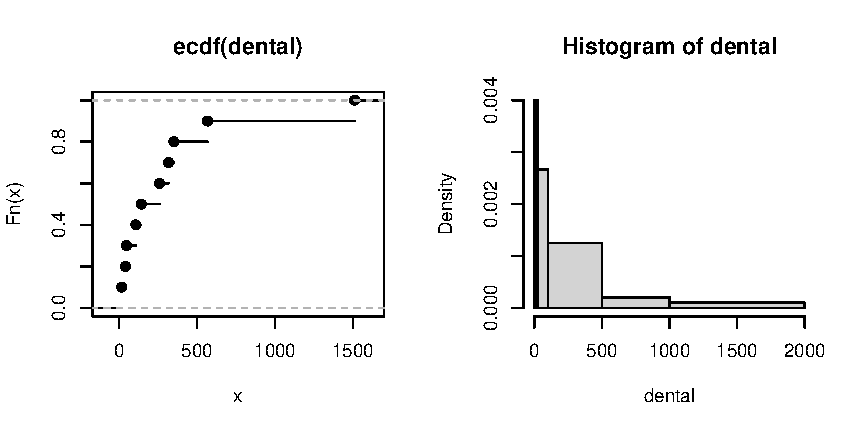
\includegraphics{cjs-rcs-figure}
%   \caption{\ifenglish A sample figure\else Exemple de figure\fi}
%   \label{fig:authguide:sample-figure}
% \end{figure}
%
% \ifenglish%
% If a figure requires an external file, you must provide it with your
% final version, usually in EPS, PDF or PNG format: see %
% \else%
% Si une figure requiert un fichier externe, vous devrez le fournir
% avec votre version finale, habituellement en format EPS, PDF ou PNG;
% consultez les %
% \fi
% \href{https://authorservices.wiley.com/author-resources/Journal-Authors/Prepare/manuscript-preparation-guidelines.html/figure-preparation.html}{%
%   \ifenglish Wiley's guidelines for the preparation of figures\relax
%   \else directives de Wiley pour la préparation des figures\fi}. %
%
% \ifenglish%
% Prepare tables as follows\relax%
% \else%
% Composez vos tableaux selon les règles suivantes\relax%
% \fi
% \footnote{%
%   \ifenglish%
%   These guidelines are adapted from the documentation of %
%   \else%
%   Ces règles sont adaptées de la documentation de %
%   \fi
%   \href{https://ctan.org/pkg/booktabs}{\pkg{booktabs}}.}: %
% \begin{itemize}
% \item %
%   \ifenglish%
%   no vertical lines; %
%   \else%
%   aucun filet vertical; %
%   \fi
% \item %
%   \ifenglish%
%   \cmdprint{\toprule} at the top; %
%   \else%
%   \cmdprint{\toprule} au début; %
%   \fi
% \item %
%   \ifenglish%
%   \cmdprint{\midrule} between the heading and body; %
%   \else%
%   \cmdprint{\midrule} entre l'entête et le corps; %
%   \fi
% \item%
%   \ifenglish%
%   \cmdprint{\bottomrule} at the bottom; %
%   \else%
%   \cmdprint{\bottomrule} au pied; %
%   \fi
% \item %
%   \ifenglish%
%   consistent number of decimal places thoughout the table; %
%   \else%
%   nombre de décimales uniforme; %
%   \fi
% \item %
%   \ifenglish%
%   leading digit in front of a decimal point ($0.1$, not $.1$).
%   \else%
%   marqueur des entiers devant les nombres décimaux ($0,1$ plutôt que
%   $,1$). %
%   \fi
% \end{itemize}
%
% \ifenglish%
% For table footnotes, use the package %
% \else%
% Pour les notes de contenu dans un tableau, utilisez %
% \fi%
% \href{https://ctan.org/pkg/threeparttable}{\pkg{threeparttable}}. %
% \ifenglish%
% However, place \cmdprint{\caption} \emph{outside} the environment
% \code{threeparttable} so that the caption can span the whole width
% of the page: %
% \else%
% Cependant, veillez à placer \cmdprint{\caption} à l'\emph{extérieur}
% de l'environnement \code{threeparttable} afin que la légende occupe
% toute la largeur de la page, le cas échéant: %
% \fi
% \iffalse
%<*example>
% \fi
  \def\CAPTION{\ifenglish caption\else légende\fi}
  \def\LABEL{\ifenglish label\else étiquette\fi}
  \def\TABLECONTENTS{\ifenglish table contents\else contenu du tableau\fi}
\begin{lstlisting}
\begin{table}
  \caption`\marg{\CAPTION}'
  \label`\marg{\LABEL}'
  \centering
  \begin{threeparttable}
    \begin{tabular}`\marg{cols}'
      `\meta{\TABLECONTENTS}'
    \end{tabular}
    \begin{tablenotes}
      `\meta{notes}'
    \end{tablenotes}
  \end{threeparttable}
\end{table}
\end{lstlisting}
% \iffalse
%</example>
% \fi
%
% \ifenglish%
% \section{Computer code and software}
% \else%
% \section{Code informatique et logiciels}
% \fi
% \label{sec:authguide:software}
%
% \ifenglish%
% Providing your computer code is a great way to increase the
% visibility of your work and its accessibility to end users of
% statistics. We strongly encourage that you share your code through a
% suitable repository, such as
% \else%
% Vous améliorerez la visibilité de vos travaux et leur dissémination
% parmi les utilisateurs de la statistique si vous fournissez votre
% code informatique. Nous vous encourageons fortement à partager
% celui-ci par le biais d'un dépôt ouvert, tel que %
% \fi
% \href{https://github.com/}{GitHub}
% \ifenglish or \else ou \fi %
% \href{https://gitlab.com/}{GitLab},
% \ifenglish%
% so that you can keep it up-to-date after the article has been
% published. Alternatively, you may provide your code in the
% Supplementary Material.
% \else%
% afin d'en permettre la mise à jour après la publication de
% l'article. Autrement, vous pouvez inclure le code dans le matériel
% additionnel. %
% \fi
%
% \ifenglish%
% The class does not offer any special features to typeset computer
% code. We recommend that you use specialized packages such
% as %
% \else%
% La classe ne propose aucune fonctionnalité particulière pour la
% présentation du code informatique. Nous vous recommandons d'avoir
% recours à des paquetages spécialisés comme %
% \fi
% \href{https://ctan.org/pkg/fancyvrb}{\pkg{fancyvrb}} %
% \ifenglish or \else ou \fi%
% \href{https://ctan.org/pkg/listings}{\pkg{listings}}. %
% \ifenglish%
% If you use {\Rlang} for your analysis, you could prepare the file
% using a literate programming system such as %
% \else%
% Si vous utilisez {\Rlang} pour effectuer votre analyse, vous pouvez
% rédiger l'article avec un système de programmation lettrée comme %
% \fi
% \href{https://en.wikipedia.org/wiki/Sweave}{Sweave} %
% \ifenglish or \else ou \fi%
% \href{https://en.wikipedia.org/wiki/Knitr}{knitr}.
%
% \ifenglish%
% That said, the class defines a few commands to ease and standardize
% the display of software names and code chunks. The command
% \cmd{\proglang} typesets the names of programming languages and
% software, and there are shortcuts for the most common cases; see
% \autoref{tab:authguide:proglang}. For example, refer to {\Rlang}
% using either \cmdprint{\proglang}\code{\{R\}} or
% \cmdprint{\Rlang}. The command \cmd{\pkg} typesets the names of
% software packages or modules. For example, refer to the {\Rlang}
% package \pkg{copula} using \cmdprint{\pkg}\code{\{copula\}}. %
% \else%
% Cela dit, la classe fournit quelques commandes pour faciliter et
% uniformiser la présentation des noms de logiciels et des extraits de
% code. La commande \cmd{\proglang} compose le nom des langages de
% programmation et des logiciels. Des raccourcis sont fournis pour les
% cas les plus usuels; voir le \autoref{tab:authguide:proglang}.
% Ainsi, pour mentionner {\Rlang}, utilisez
% \cmdprint{\proglang}\code{\{R\}} ou \cmdprint{\Rlang}. La commande
% \cmd{\pkg} compose le nom des paquetages ou modules logiciels. Par
% exemple, vous saisirez \cmdprint{\pkg}\code{\{copula\}} pour
% mentionner le paquetage {\Rlang} \pkg{copula}. %
% \fi
%
% \begin{table}
%   \ifenglish%
%   \caption{List of shortcuts for the names of programming languages
%   and software.}
%   \else%
%   \caption{Liste des raccourcis pour les noms de langages de
%   programmation et de logiciels}
%   \fi
%   \label{tab:authguide:proglang}
%   \centering
%   \begin{tabular}{ll}
%     \toprule
%     \ifenglish Software\else Logiciel\fi & \ifenglish Command\else Commande\fi \\
%     \midrule
%     \Rlang     & \cmd{\Rlang} \\
%     \SASlang   & \cmd{\SASlang} \\
%     \SPSSlang  & \cmd{\SPSSlang} \\
%     \Statalang & \cmd{\Statalang} \\
%     \Pylang    & \cmd{\Pylang} \\
%     \Julialang & \cmd{\Julialang} \\
%     \Clang     & \cmd{\Clang} \\
%     \Cpplang   & \cmd{\Cpplang} \\
%     \bottomrule
%   \end{tabular}
% \end{table}
%
% \ifenglish%
% For small chunks of code, such as the names of exploratory variables
% in a regression model, \cmd{\code} may be useful: it allows you to
% use the characters \code{_}, \code{~} and \code{$} directly. For
% example, you may write \cmdprint{\code}\code{\{patient_age\}} to get
% \code{patient_age}. %
% \else%
% La commande \cmd{\code} est utile pour composer de courts extraits
% de code, comme les noms des variables d'un modèle de régression. La
% commande permet d'utiliser directement les caractères «\code{_}»,
% «\code{~}» et «\code{$}». Par exemple, vous pouvez entrer
% \cmdprint{\code}\code{\{patient_age\}} pour obtenir
% \code{patient_age}. %
% \fi
%
% \ifenglish%
% Remember to report the software packages you used and their
% version numbers; see the following section. %
% \else%
% Vous devez toujours mentionner les logiciels utilisés, ainsi que
% leur version. La section suivante fournit plus de détails à ce
% sujet.
% \fi
%
% \ifenglish%
% \section{Citations and references}
% \else%
% \section{Citations et références}
% \fi
% \label{sec:authguide:references}
%
% \ifenglish%
% For citations and references, use {\BibTeX}. Recall that %
% \else%
% Utilisez {\BibTeX} pour les citations et les références. Tel que
% mentionné précédemment, le paquetage %
% \fi%
% \href{https://ctan.org/pkg/natbib}{\pkg{natbib}} %
% \ifenglish%
% is loaded automatically. Please use the \cmd{\citet} and
% \cmd{\citep} commands of \pkg{natbib}.
% \else%
% est chargé automatiquement par la classe. Assurez-vous
% d'utiliser ses commandes \cmd{\citet} et \cmd{\citep}. %
% \fi
%
% \ifenglish%
% The class also uses its own bibliography styles. These styles
% support the standard {\BibTeX} entry types %
% \else%
% La classe a également recours à ses propres styles de bibliographie.
% Ceux-ci prennent en charge les types d'entrées standards de
% {\BibTeX} %
% \fi
% (\code{article}, \code{book}, \code{proceedings}, etc.) %
% \ifenglish%
% and the standard fields %
% \else%
% et les champs standards %
% \fi%
% (\code{author}, \code{title}, \code{journal}, etc.). %
% \ifenglish%
% Furthermore, the styles support %
% \else%
% De plus, ils ajoutent les champs %
% \fi%
% \code{doi}, \code{isbn}, \code{url} \ifenglish and \else et \fi
% \code{language}.
% \ifenglish%
% These are explained in the examples below. %
% \else%
% Les exemples ci-dessous illustrent chacun de ces champs. %
% \fi%
%
% \begin{itemize}
% \item %
%   \ifenglish%
%   Articles with one author: \citet{Genest:1999}. To include a
%   DOI, use the field \code{doi} with a value in the format
%   \meta{prefix}\code{/}\meta{suffix} (for example,
%   \code{10.2307/3315650}). A hyperlink to the resource is then
%   created automatically. Note that journal names should not be
%   abbreviated. %
%   \else%
%   Articles avec un auteur unique: \citet{Genest:1999}. Pour ajouter
%   un identificateur DOI, utilisez le champ \code{doi} avec une valeur
%   de la forme \meta{préfixe}\code{/}\meta{suffixe} (par exemple:
%   \code{10.2307/3315650}). Un hyperlien vers la ressource est créé
%   automatiquement. Inscrivez les noms des journaux au long. %
%   \fi
% \item %
%   \ifenglish%
%   Articles with two authors: \citet{Qin/Lawless:1995}. Articles
%   with three or more authors: \citet{Davison/Fraser/Reid:2006} or
%   \citet{Granville:2023}. For articles with more than ten authors
%   \citep[such as][]{Teufel:2016}, give the first seven names
%   followed by ``and others''. {\BibTeX} will replace this by
%   ``et~al.''
%   \else%
%   Articles avec deux auteurs: \citet{Qin/Lawless:1995}. Articles
%   avec trois auteurs ou plus: \citet{Davison/Fraser/Reid:2006} ou
%   encore \citet{Granville:2023}. Pour les articles comptant plus de
%   dix auteurs \citep[par exemple:][]{Teufel:2016}, inscrivez les
%   noms des sept premiers auteurs, suivis de \emph{and others}.
%   {\BibTeX} inscrira automatiquement «et collab.» dans la notice.
%   \fi
% \item %
%   \ifenglish%
%   Use the field \code{language} for foreign-language articles, as in
%   \citet{Hoeffding:1940} (German) or
%   \citet{Ghoudi/Khoudraji/Rivest:1998} (French). Including this
%   information in the {\BibTeX} entry ensures that the title words
%   are hyphenated according to the rules of the corresponding
%   language. %
%   \else%
%   Le champ \code{language} permet d'indiquer la langue d'une notice
%   lorsqu'elle diffère de celle de l'article. C'est important pour la
%   coupure de mots dans les titres. Par exemple, pour le présent
%   document en français, la plupart des entrées de la bibliographie
%   déclarent l'anglais comme langue, alors que \citet{Hoeffding:1940}
%   déclare l'allemand. En revanche,
%   \citet{Ghoudi/Khoudraji/Rivest:1998} déclare le français pour la
%   version anglaise du document. %
%   \fi
% \item %
%   \ifenglish%
%   Books and other formats use the same author rules as articles.
%   An example of a book with two authors is
%   \citet{Kalbfleisch/Prentice:2002}. You may use \code{isbn} to include
%   the book's ISBN. Include the relevant page, section, or chapter
%   whenever possible in \cmd{\citet} and \cmd{\citep}. For example,
%   partial likelihood estimation in the Cox regression model may be
%   found in %
%   \else%
%   Les règles pour les auteurs de livres et autres types d'entrées
%   sont les mêmes que pour les articles.
%   \citet{Kalbfleisch/Prentice:2002} est un exemple de livre comptant
%   deux auteurs. Utilisez le champ \code{isbn} pour préciser le
%   numéro ISBN de l'ouvrage. Quand vous citez un livre, précisez
%   autant que faire se peut la page, la section ou le chapitre dans
%   les commandes \cmd{\citet} et \cmd{\citep}. Par exemple,
%   l'estimation par vraisemblance partielle dans le modèle de
%   régression de Cox est traitée dans %
%   \fi
%   \citet[\ifenglish Section\else section\fi~4.2]{Kalbfleisch/Prentice:2002}; %
%   \ifenglish see also \else voir aussi \fi %
%   \citet[\ifenglish Chapter\else chapitre\fi~6]{Kalbfleisch/Prentice:2002}.
% \item %
%   \ifenglish%
%   For references to articles in an edited book, include the page
%   numbers of the article, as well as the names of the book's
%   editors, such as \citet{Roberts:2009}. Again, we encourage you to
%   include the DOI. %
%   \else%
%   Pour la notice d'une partie d'un ouvrage collectif, précisez les
%   pages de la partie citée ainsi que les noms des éditeurs, tel que
%   dans \citet{Roberts:2009}. Ici aussi, nous vous invitons à inclure
%   un identificateur DOI. %
%   \fi
% \item %
%   \ifenglish%
%   You may need to cite a PhD thesis such as \citet{Syed:2022} or a
%   technical report such as \citet{Haas:2001} or an unpublished
%   manuscript posted on arXiv such as \citet{Tang/Kong/Wang:2023}.
%   If you have a DOI or URL, include it in the entry using \code{doi}
%   or \code{url}. If both are present in the database, the DOI
%   takes precedence.
%   \else%
%   Vous pouvez citer une thèse de doctorat \citep{Syed:2022}, un
%   rapport technique \citep{Haas:2001} ou une publication
%   préliminaire dans arXiv \citep{Tang/Kong/Wang:2023}. Saisissez les
%   identificateur DOI et les adresses URL avec les champs \code{doi}
%   et \code{url}. Lorsque les deux sont présents dans la base de
%   données, l'identificateur DOI a priorité. %
%   \fi
% \item %
%   \ifenglish%
%   Cite the software you used in your statistical analysis,
%   especially Free Software. To cite {\Rlang}, use the {\BibTeX}
%   entry provided by the command %
%   \else%
%   Citez les logiciels utilisés pour vos analyses statistiques, tout
%   particulièrement les logiciels libres. Pour citer {\Rlang},
%   utilisez l'entrée {\BibTeX} produite par la commande %
%   \fi
% \iffalse
%<*example>
% \fi
\begin{lstlisting}
> citation()
\end{lstlisting}
% \iffalse
%</example>
% \fi
%   \ifenglish%
%   Don't forget to include the version of {\Rlang}, as in:
%   ``Computations in this article were performed using {\Rlang}
%   \citep[v4.5.0]{Rlang}''. You can get this via:
%   \else%
%   N'oubliez pas d'inclure aussi la version de {\Rlang} dans une
%   mention de la forme «Les calculs de cet article ont été effectués
%   avec {\Rlang} \citep[v4.5.0]{Rlang}». L'expression {\Rlang}
%   suivante fournit la version du logiciel: %
%   \fi
% \iffalse
%<*example>
% \fi
\begin{lstlisting}
> R.version.string
\end{lstlisting}
% \iffalse
%</example>
% \fi
%   \ifenglish%
%   To cite an {\Rlang} package, use the command \code{citation} with
%   the name of the package in argument, e.g.\ %
%   \else%
%   Pour citer un paquetage {\Rlang}, utilisez aussi la commande
%   \code{citation}, mais en ajoutant le nom du paquetage en
%   argument: %
%   \fi
% \iffalse
%<*example>
% \fi
\begin{lstlisting}
> citation("copula")
\end{lstlisting}
% \iffalse
%</example>
% \fi
%   \ifenglish%
%   This specific example asks you to cite three articles
%   \citep{Yan:2007,Kojadinovic/Yan:2010,Hofert/Maechler:2011} as well
%   as the software itself \citep{Rcopula:2024}.
%   \else%
%   Dans cet exemple en particulier, on demande de citer trois
%   articles
%   \citep{Yan:2007,Kojadinovic/Yan:2010,Hofert/Maechler:2011} en plus
%   du logiciel lui-même \citep{Rcopula:2024}. %
%   \fi
% \item %
%   \ifenglish%
%   To cite data, please review %
%   \else%
%   Si vous devez citer des données, consultez la %
%   \fi
%   \href{https://authorservices.wiley.com/author-resources/Journal-Authors/open-access/data-sharing-citation/data-citation-policy.html}{%
%     \ifenglish Wiley's data citation policy\relax
%     \else politique de citation des données de Wiley\fi}. %
%   \ifenglish%
%   An example of a data citation is \citet{StatCan:2023}.
%   \else%
%   Un exemple de citation de données est \citet{StatCan:2023-fr}.
%   \fi
% \item %
%   \ifenglish%
%   You can also cite a webpage, for example \citet{Wolfram:2010}.
%   Include the date of access using the \code{note} field. %
%   \else%
%   Vous pouvez citer une page web, par exemple \citet{Wolfram:2010}.
%   Précisez la date de consultation de la page dans le champ
%   \code{note}. %
%   \fi
% \end{itemize}
%
% \appendix
%
% \ifenglish%
% \section{Proofs}
% \else%
% \section{Démonstrations}
% \fi
% \label{sec:authguide:proofs}
%
% \ifenglish%
% Appendices usually present original proofs or longer mathematical
% derivations; don't forget to cite them in the main article. You
% may structure each appendix into multiple sections and
% subsections. %
% \else%
% Les annexes sont habituellement réservées aux démonstrations ou
% longs développements mathématiques. Vous devez les citer dans le
% corps de l'article. Vous pouvez diviser les annexes en sections et
% sous-sections. %
% \fi
%
% \ifenglish%
% \section{Supplementary material}
% \else%
% \section{Matériel additionnel}
% \fi
% \label{sec:authguide:supplement}
%
% \ifenglish%
% To make your article accessible to a wide readership and to control
% its length, consider providing online supplementary material, citing
% it in the main article. It may contain additional simulation
% results, lengthy tables or figures, auxiliary results, proofs that
% are direct adaptations of calculations already published elsewhere,
% details about the code and software implementation, and so on. That
% said, we encourage you to place original mathematical proofs in an
% appendix and to present the ideas behind these proofs in the main
% text. %
% \else%
% Le matériel additionnel rendu disponible en ligne permet d'élargir
% le lectorat de votre article tout en limitant sa longueur. Vous
% devez citer le matériel additionnel dans l'article. Celui-ci peut
% contenir, entre autres, des résultats de simulation additionnels, de
% longs tableaux ou de grandes figures, des résultats auxiliaires, des
% démonstrations qui sont des applications directes de résultats déjà
% publiés ailleurs, des détails à propos de la mise en œuvre
% informatique. Attention, toutefois: les démonstrations originales
% sont mieux à leur place dans une annexe. Présentez simplement les
% idées fortes derrière celles-ci dans le corps du texte. %
% \fi
%
% \ifenglish%
% To prepare the supplementary material, use the option
% \code{supplement}: %
% \else%
% Pour préparer le matériel additionnel, utilisez l'option
% \code{supplement} de la classe: %
% \fi
% \iffalse
%<*example>
% \fi
\begin{lstlisting}
\documentclass[`\LANGOPT',supplement]{cjs-rcs-article}
\end{lstlisting}
% \iffalse
%</example>
% \fi
% \ifenglish%
% or, to make the supplement suitable for review, %
% \else%
% ou, pour anonymiser le matériel additionnel en vue de l'évaluation
% par les pairs,
% \fi
% \iffalse
%<*example>
% \fi
\begin{lstlisting}
\documentclass[`\LANGOPT',supplement,review]{cjs-rcs-article}
\end{lstlisting}
% \iffalse
%</example>
% \fi
% \ifenglish%
% Your supplementary material is published as supplied, and a proof is
% not made available, so be sure to double-check the file and to
% provide the material in its final format. %
% \else%
% Nous publions votre matériel additionnel tel quel; aucune épreuve ne
% vous sera fournie. Assurez-vous donc de la conformité de votre
% fichier. %
% \fi
%
% \vspace*{10pt}
% \hfill
% \ifenglish%
%   \emph{Have fun writing!}
% \else%
%   \emph{Bonne rédaction!}
% \fi%
%
% \begin{thebibliography}{23}
% \providecommand{\natexlab}[1]{#1}
% \providecommand{\url}[1]{\texttt{#1}}
% \providecommand{\urlprefix}{}
% \providecommand{\doiprefix}{doi: }
% \expandafter\ifx\csname href\endcsname\relax
%   \providecommand{\urldoi}[1]{#1}\else
%   \providecommand{\urldoi}[1]{\href{https://doi.org/#1}{#1}}\fi
% \providecommand{\selectlanguage}[1]{\relax}
% 
% \bibitem[{Davison et~al.(2006)Davison, Fraser, and
%   Reid}]{Davison/Fraser/Reid:2006}
% Davison, A.~C., Fraser, D. A.~S., and Reid, N. (2006).
% \newblock {\selectlanguage{english}Improved likelihood inference for discrete
%   data}.
% \newblock \emph{Journal of the Royal Statistical Society Series B: Statistical
%   Methodology}, 68(3):495--508.
% \newblock \doiprefix\urldoi{10.1111/j.1467-9868.2006.00548.x}.
% 
% \bibitem[{Downes and Beeton(2017)}]{Downes:short-math-guide:2017}
% Downes, M. and Beeton, B. (2017).
% \newblock {\selectlanguage{english}\emph{Short Math Guide for {\LaTeX}}}.
% \newblock American Mathematical Society.
% \newblock \urlprefix\url{https://ctan.org/pkg/short-math-guide}.
% 
% \bibitem[{Genest(1999)}]{Genest:1999}
% Genest, C. (1999).
% \newblock {\selectlanguage{english}Probability and statistics: A tale of two
%   worlds?}
% \newblock \emph{The Canadian Journal of Statistics}, 27(2):421--444.
% \newblock \doiprefix\urldoi{10.2307/3315650}.
% 
% \bibitem[{Ghoudi et~al.(1998)Ghoudi, Khoudraji, and
%   Rivest}]{Ghoudi/Khoudraji/Rivest:1998}
% Ghoudi, K., Khoudraji, A., and Rivest, L.-P. (1998).
% \newblock {\selectlanguage{french}Propri\'et\'es statistiques des copules de
%   valeurs extr\^emes bidimensionnelles}.
% \newblock \emph{The Canadian Journal of Statistics}, 26:187--197.
% \newblock \doiprefix\urldoi{10.2307/3315683}.
% 
% \bibitem[{Granville et~al.(2023)Granville, Woolford, Dean, Boychuk, and
%   McFayden}]{Granville:2023}
% Granville, K., Woolford, D.~G., Dean, C.~B., Boychuk, D., and McFayden, C.~B.
%   (2023).
% \newblock {\selectlanguage{english}On the selection of an interpolation method
%   with an application to the {F}ire {W}eather {I}ndex in {O}ntario, {C}anada}.
% \newblock \emph{Environmetrics}, 34(2):e2758.
% \newblock \doiprefix\urldoi{10.1002/env.2758}.
% 
% \bibitem[{Haas(2001)}]{Haas:2001}
% Haas, M. (2001).
% \newblock {\selectlanguage{english}\emph{New Methods in Backtesting}}.
% \newblock Tech. rep., Financial Engineering Research Center, Bonn, Germany.
% \newblock \urlprefix\url{https://www.yumpu.com/s/L9EC3aHSgRvWa763}.
% 
% \bibitem[{Higham(2020)}]{Higham:2020}
% Higham, N.~J. (2020).
% \newblock {\selectlanguage{english}\emph{Handbook of Writing for the
%   Mathematical Sciences}}.
% \newblock 3rd ed. SIAM, Philadelphia.
% \newblock ISBN 978-1-61197-609-0.
% \newblock \doiprefix\urldoi{10.1137/1.9781611976106}.
% 
% \bibitem[{Hoeffding(1940)}]{Hoeffding:1940}
% Hoeffding, W. (1940).
% \newblock {\selectlanguage{german}Ma{\ss}stabinvariante {K}orrelationstheorie
%   f\"ur diskontinuierliche {V}erteilungen}.
% \newblock \emph{Archiv f\"ur mathematische Wirtschafts- und Sozialforschung},
%   7:4--70.
% 
% \bibitem[{Hofert et~al.(2023)Hofert, Kojadinovic, Maechler, and
%   Yan}]{Rcopula:2024}
% Hofert, M., Kojadinovic, I., Maechler, M., and Yan, J. (2023).
% \newblock {\selectlanguage{english}\emph{copula: Multivariate Dependence with
%   Copulas}}.
% \newblock \urlprefix\url{https://cran.r-project.org/package=copula}.
% \newblock R package version 1.1-4.
% 
% \bibitem[{Hofert and M\"achler(2011)}]{Hofert/Maechler:2011}
% Hofert, M. and M\"achler, M. (2011).
% \newblock {\selectlanguage{english}Nested {A}rchimedean copulas meet {R}: The
%   {nacopula} package}.
% \newblock \emph{Journal of Statistical Software}, 39(9):1--20.
% \newblock \doiprefix\urldoi{10.18637/jss.v039.i09}.
% 
% \bibitem[{Kalbfleisch and Prentice(2002)}]{Kalbfleisch/Prentice:2002}
% Kalbfleisch, J.~D. and Prentice, R.~L. (2002).
% \newblock {\selectlanguage{english}\emph{The Statistical Analysis of Failure
%   Time Data}}.
% \newblock 2nd ed. Wiley Series in Probability and Statistics,
%   Wiley-Interscience [John Wiley \& Sons], Hoboken, NJ.
% \newblock ISBN 9780471363576.
% \newblock \doiprefix\urldoi{10.1002/9781118032985}.
% 
% \bibitem[{Kojadinovic and Yan(2010)}]{Kojadinovic/Yan:2010}
% Kojadinovic, I. and Yan, J. (2010).
% \newblock {\selectlanguage{english}Modeling multivariate distributions with
%   continuous margins using the {copula} {R} package}.
% \newblock \emph{Journal of Statistical Software}, 34(9):1--20.
% \newblock \doiprefix\urldoi{10.18637/jss.v034.i09}.
% 
% \bibitem[{Mermin(1989)}]{Mermin:1989}
% Mermin, N.~D. (1989).
% \newblock {\selectlanguage{english}What's wrong with these equations?}
% \newblock \emph{Physics Today}, 42(10):9--11.
% \newblock \doiprefix\urldoi{10.1063/1.2811173}.
% 
% \bibitem[{Oetiker et~al.(2021)Oetiker, Partl, Hyna, and
%   Schlegl}]{Oetiker:lshort-english:2021}
% Oetiker, T., Partl, H., Hyna, I., and Schlegl, E. (2021).
% \newblock {\selectlanguage{english}\emph{The Not So Short Introduction to
%   {\LaTeXe}}}.
% \newblock \urlprefix\url{https://ctan.org/pkg/lshort-english}.
% \newblock Version 6.4.
% 
% \bibitem[{Qin and Lawless(1995)}]{Qin/Lawless:1995}
% Qin, J. and Lawless, J. (1995).
% \newblock {\selectlanguage{english}Estimating equations, empirical likelihood
%   and constraints on parameters}.
% \newblock \emph{The Canadian Journal of Statistics}, 23(2):145--159.
% \newblock \doiprefix\urldoi{10.2307/3315441}.
% 
% \bibitem[{{R Core Team}(2024)}]{Rlang}
% {R Core Team} (2024).
% \newblock {\selectlanguage{english}\emph{R: A Language and Environment for
%   Statistical Computing}}.
% \newblock R Foundation for Statistical Computing, Vienna, Austria.
% \newblock \urlprefix\url{https://www.r-project.org/}.
% 
% \bibitem[{Roberts et~al.(2009)Roberts, Ren, and Rao}]{Roberts:2009}
% Roberts, G., Ren, Q., and Rao, J. N.~K. (2009).
% \newblock {\selectlanguage{english}Using marginal mean models for data from
%   longitudinal surveys with a complex design: Some advances in methods}.
% \newblock In R.~Lynn, editor, \emph{Methodology of Longitudinal Surveys}, pages
%   351--366. John Wiley \& Sons, New York.
% \newblock ISBN 9780470018712.
% \newblock \doiprefix\urldoi{10.1002/9780470743874}.
% 
% \bibitem[{{Statistics Canada}(2023)}]{StatCan:2023}
% {Statistics Canada} (2023).
% \newblock {\selectlanguage{english}Table 13-10-0096-01 {H}ealth
%   characteristics, annual estimates, inactive}.
% \newblock \doiprefix\urldoi{10.25318/1310009601-eng}.
% 
% \bibitem[{Syed(2022)}]{Syed:2022}
% Syed, S. (2022).
% \newblock {\selectlanguage{english}\emph{Non-reversible parallel tempering on
%   optimized paths}}.
% \newblock Ph.D. thesis, University of British Columbia, Vancouver (BC), Canada.
% \newblock \doiprefix\urldoi{10.14288/1.0413120}.
% 
% \bibitem[{Tang et~al.(2023)Tang, Kong, and Wang}]{Tang/Kong/Wang:2023}
% Tang, D., Kong, D., and Wang, L. (2023).
% \newblock {\selectlanguage{english}The synthetic instrument: From sparse
%   association to sparse causation}.
% \newblock arXiv.
% \newblock \doiprefix\urldoi{10.48550/arXiv.2304.01098}.
% 
% \bibitem[{Teufel et~al.(2016)Teufel, Diro, Whan, Milrad, Jeong, Ganji, Huziy
%   et~al.}]{Teufel:2016}
% Teufel, B., Diro, G.~T., Whan, K., Milrad, S.~M., Jeong, D.~I., Ganji, A.,
%   Huziy, O. et~al. (2016).
% \newblock {\selectlanguage{english}Investigation of the 2013 {A}lberta flood
%   from a weather/climate perspective}.
% \newblock \emph{Climate Dynamics}, 48(9):2881--2899.
% \newblock \doiprefix\urldoi{10.1007/s00382-016-3239-8}.
% 
% \bibitem[{{W}olfram {R}esearch(2010)}]{Wolfram:2010}
% {W}olfram {R}esearch (2010).
% \newblock {\selectlanguage{english}Pearson distribution}.
% \newblock
%   \urlprefix\url{https://reference.wolfram.com/language/ref/PearsonDistribution.html}.
% \newblock Accessed October 12, 2022.
% 
% \bibitem[{Yan(2007)}]{Yan:2007}
% Yan, J. (2007).
% \newblock {\selectlanguage{english}Enjoy the joy of copulas: With a package
%   copula}.
% \newblock \emph{Journal of Statistical Software}, 21(4):1--21.
% \newblock \doiprefix\urldoi{10.18637/jss.v021.i04}.
% 
% \end{thebibliography}
%
% \ifenglish%
%   \PrintChanges
% \else%
%   \section*{Historique des versions}
%   \label{sec:authguide:implementation}
%   Consultez la version anglaise de ce document pour l'historique des
%   versions. %
% \fi
